\documentclass{headers/polimi_3i}

%------------------------------------------------------------------------------
%	REQUIRED PACKAGES AND  CONFIGURATIONS
%------------------------------------------------------------------------------

% CONFIGURATIONS
\usepackage{parskip} % For paragraph layout
\usepackage{setspace} % For using single or double spacing
\usepackage{emptypage} % To insert empty pages
\usepackage{multicol} % To write in multiple columns (executive summary)
\setlength\columnsep{15pt} % Column separation in executive summary
\setlength\parindent{0pt} % Indentation
\raggedbottom  

% PACKAGES FOR TITLES
\usepackage{titlesec}
% \titlespacing{\section}{left spacing}{before spacing}{after spacing}
\titlespacing{\section}{0pt}{3.3ex}{2ex}
\titlespacing{\subsection}{0pt}{3.3ex}{1.65ex}
\titlespacing{\subsubsection}{0pt}{3.3ex}{1ex}
\usepackage{color}

% PACKAGES FOR LANGUAGE AND FONT
\usepackage[english]{babel} % The document is in English  
\usepackage[utf8]{inputenc} % UTF8 encoding
\usepackage[T1]{fontenc} % Font encoding
\usepackage[11pt]{moresize} % Big fonts

% PACKAGES FOR IMAGES
\usepackage{graphicx}
\usepackage{transparent} % Enables transparent images
\usepackage{eso-pic} % For the background picture on the title page
%\usepackage{subfig} % Numbered and caption subfigures using \subfloat.
\usepackage{tikz} % A package for high-quality hand-made figures.
\usetikzlibrary{}
\graphicspath{{./images/}} % Directory of the images
\usepackage{caption} % Coloured captions
\usepackage{subcaption} % Subfigures
\usepackage{xcolor} % Coloured captions
\usepackage{amsthm,thmtools,xcolor} % Coloured "Theorem"
\usepackage{float}

% STANDARD MATH PACKAGES
\usepackage{amsmath}
\usepackage{amsthm}
\usepackage{amssymb}
\usepackage{amsfonts}
\usepackage{bm}
\usepackage[overload]{empheq} % For braced-style systems of equations.
\usepackage{fix-cm} % To override original LaTeX restrictions on sizes

% PACKAGES FOR TABLES
\usepackage{tabularx}
\usepackage{longtable} % Tables that can span several pages
\usepackage{colortbl}

% PACKAGES FOR ALGORITHMS (PSEUDO-CODE)
\usepackage{algorithm}
\usepackage{algpseudocode}

% PACKAGES FOR REFERENCES & BIBLIOGRAPHY
\usepackage[colorlinks=true,linkcolor=black,anchorcolor=black,citecolor=black,filecolor=black,menucolor=black,runcolor=black,urlcolor=black]{hyperref} % Adds clickable links at references
\usepackage{cleveref}
%\usepackage[square, numbers, sort&compress]{natbib} % Square brackets, citing references with numbers, citations sorted by appearance in the text and compressed
%\bibliographystyle{abbrvnat} % You may use a different style adapted to your field

% OTHER PACKAGES
\usepackage{pdfpages} % To include a pdf file
\usepackage{afterpage}
\usepackage{lipsum} % DUMMY PACKAGE
\usepackage{fancyhdr} % For the headers

\fancyhf{}

% Input of configuration file. Do not change config.tex file unless you really know what you are doing. 
% Define blue color typical of polimi
\definecolor{bluepoli}{cmyk}{0.4,0.1,0,0.4}

% Custom theorem environments
\declaretheoremstyle[
  headfont=\color{bluepoli}\normalfont\bfseries,
  bodyfont=\color{black}\normalfont\itshape,
]{colored}

% Set-up caption colors
\captionsetup[figure]{labelfont={color=bluepoli}} % Set colour of the captions
\captionsetup[table]{labelfont={color=bluepoli}} % Set colour of the captions
\captionsetup[algorithm]{labelfont={color=bluepoli}} % Set colour of the captions

\theoremstyle{colored}
\newtheorem{theorem}{Theorem}[chapter]
\newtheorem{proposition}{Proposition}[chapter]

% Enhances the features of the standard "table" and "tabular" environments.
\newcommand\T{\rule{0pt}{2.6ex}}
\newcommand\B{\rule[-1.2ex]{0pt}{0pt}}

% Pseudo-code algorithm descriptions.
\newcounter{algsubstate}
\renewcommand{\thealgsubstate}{\alph{algsubstate}}
\newenvironment{algsubstates}
  {\setcounter{algsubstate}{0}%
   \renewcommand{\STATE}{%
     \stepcounter{algsubstate}%
     \Statex {\small\thealgsubstate:}\space}}
  {}

% New font size
\newcommand\numfontsize{\@setfontsize\Huge{200}{60}}

% Title format: chapter
\titleformat{\chapter}[hang]{
\fontsize{50}{20}\selectfont\bfseries\filright}{\textcolor{bluepoli} \thechapter\hsp\hspace{2mm}\textcolor{bluepoli}{|   }\hsp}{0pt}{\huge\bfseries \textcolor{bluepoli}
}

% Title format: section
\titleformat{\section}
{\color{bluepoli}\normalfont\Large\bfseries}
{\color{bluepoli}\thesection.}{1em}{}

% Title format: subsection
\titleformat{\subsection}
{\color{bluepoli}\normalfont\large\bfseries}
{\color{bluepoli}\thesubsection.}{1em}{}

% Title format: subsubsection
\titleformat{\subsubsection}
{\color{bluepoli}\normalfont\large\bfseries}
{\color{bluepoli}\thesubsubsection.}{1em}{}

% Shortening for setting no horizontal-spacing
\newcommand{\hsp}{\hspace{0pt}}

\makeatletter
% Renewcommand: cleardoublepage including the background pic
\renewcommand*\cleardoublepage{%
  \clearpage\if@twoside\ifodd\c@page\else
  \null
  \AddToShipoutPicture*{\BackgroundPic}
  \thispagestyle{empty}%
  \newpage
  \if@twocolumn\hbox{}\newpage\fi\fi\fi}
\makeatother

%For correctly numbering algorithms
\numberwithin{algorithm}{chapter}

%----------------------------------------------------------------------------
%	NEW COMMANDS DEFINED
%----------------------------------------------------------------------------

%----------------------------------------------------------------------------
%	ADD YOUR PACKAGES (be careful of package interaction)
%----------------------------------------------------------------------------

\usepackage{enumitem}

\usepackage[style=numeric, sorting=nyt]{biblatex}

\addbibresource{chapters/biblio.bib}

\usepackage{listings}
\usepackage{color}
\definecolor{gray}{rgb}{0.4,0.4,0.4}
\definecolor{darkblue}{rgb}{0.0,0.0,0.6}
\definecolor{cyan}{rgb}{0.0,0.6,0.6}

%----------------------------------------------------------------------------
%	ADD YOUR DEFINITIONS AND COMMANDS (be careful of existing commands)
%----------------------------------------------------------------------------

%todo box highlight
\newcommand{\TODO}[1]{\noindent\colorbox{orange}{
	\parbox{\dimexpr\linewidth-2\fboxsep}
	{\textcolor{black}{\textbf{TODO:} #1}}}\par}

% Define a custom command for the list inside a table
% inserts padding on top and bottom, and no left indentation
\newcommand{\customtablelist}[1]{%
	\noindent
	\begin{minipage}[c]{6cm}
		\raggedright
		\begin{itemize}[left=0pt, after=\strut, before=\vskip 8pt]
			#1
		\end{itemize}
	\end{minipage}
}

\hyphenation{Interpret-ability}


\lstset{
	basicstyle=\footnotesize\ttfamily,
	columns=fullflexible,
	showstringspaces=false,
	commentstyle=\color{gray}\upshape,
	frame=single, % Add a frame around the code
	tabsize=4, % Set the tab size to 2 spaces
	breaklines=true, % Allow line breaks
	captionpos=b, % Set the caption position to bottom
	numbers=left, % Show line numbers on the left
	numberstyle=\tiny\color{gray}, % Set the style of line numbers to tiny gray
}

\lstdefinelanguage{XML}{
	morestring=[b]",
	morestring=[s]{>}{<},
	morecomment=[s]{<?}{?>},
	stringstyle=\color{black},
	identifierstyle=\color{darkblue},
	keywordstyle=\color{cyan},
	morekeywords={xmlns,Domain,type}% list your attributes here
}

%----------------------------------------------------------------------------
%	BEGIN OF YOUR DOCUMENT
%----------------------------------------------------------------------------

\begin{document}

\fancypagestyle{plain}{%
	\fancyhf{} % Clear all header and footer fields
	\fancyhead[RO,RE]{\thepage} %RO=right odd, RE=right even
	\renewcommand{\headrulewidth}{0pt}
	\renewcommand{\footrulewidth}{0pt}}

%----------------------------------------------------------------------------
%	TITLE PAGE
%----------------------------------------------------------------------------

\pagestyle{empty} % No page numbers
\frontmatter % Use roman page numbering style (i, ii, iii, iv...) for the preamble pages

\puttitle{  % These info will be put into your Title page 
	% Title of the thesis
	title=Development of an Autonomous Mobile Manipulation Robot for \\Industrial and Agricultural \\Environments,
	name=Simone Giampà, % Author Name and Surname
	course=Computer Science Engineering, % Study Programme
	ID  = 980857,  % Student ID number
	advisor= Prof. Matteo Matteucci, % Supervisor name
	coadvisor=Dr. Gianluca Bardaro, % Co-Supervisor name, remove this line if there is none
	academicyear={2023-24},  % Academic Year
}

%----------------------------------------------------------------------------
%	PREAMBLE PAGES: ABSTRACT (inglese e italiano), EXECUTIVE SUMMARY
%----------------------------------------------------------------------------

\thispagestyle{empty} % Remove page number for this page
\vspace*{\fill} % Push the quote to the vertical center of the page
\begin{flushright}
	\textit{"Any sufficiently advanced technology is indistinguishable from magic."}

	\bigskip % Add extra space between quote and author

	--  \textit{Arthur C. Clarke}
\end{flushright}
\vspace*{\fill}

\startpreamble
\setcounter{page}{1} % Set page counter to 1

% ABSTRACT IN ENGLISH and ITALIAN

% ABSTRACT IN ENGLISH
\chapter*{Abstract}

This thesis explores the development of a cost-effective, autonomous mobile manipulation robot designed 
to address complex tasks in industrial and agricultural environments. The system integrates a mobile platform with
a robotic arm, leveraging the ROS2 robotics framework, Nav2 for autonomous navigation, and MoveIt2 for motion planning. 
A primary focus is the design and implementation of a pneumatic soft gripper, supported by 3D-printed components, 
to enable delicate object manipulation.
The project addresses the challenges of creating a fully autonomous system capable of operating in dynamic,
unstructured environments. This involves the fusion of various sensor data, the development 
of robust algorithms for perception and object manipulation, and the seamless integration of diverse hardware
and software components. Rigorous testing in both simulated and real-world scenarios, mimicking realistic 
agricultural and industrial settings, ensures the system's practicality and effectiveness.

Key contributions include a modular software architecture that facilitates future developments to the project,
software libraries for perception, and a successful demonstration of complex 
tasks involving both robots. The project also investigates the use of a soft gripper,
highlighting its advantages in handling delicate items with its deformable nature.
The thesis successfully answers the questions posed at its outset, demonstrating the feasibility of constructing 
a capable mobile manipulator by combining existing robotic platforms. The solution demonstrates a cost-effective 
approach to automation, leveraging affordable components and open-source software frameworks. 
It showcases the system's ability to perform intricate tasks, such as picking and placing objects,
navigating autonomously, and adapting to dynamic environments.

The results of this research hold significant promise for a variety of applications in agriculture and industry.
The developed mobile manipulator can enhance productivity, efficiency, and safety by automating repetitive and potentially 
hazardous tasks. Furthermore, the modular design provides a foundation for future 
research and development in this field, fostering the creation of even more adaptable and intelligent robotic systems.

\textbf{Keywords}: Mobile Manipulation, Autonomous Navigation, Soft Robotics, ROS2, MoveIt2

% ABSTRACT IN ITALIAN
\chapter*{Abstract in lingua italiana}

Questa tesi esplora lo sviluppo di un robot mobile per la manipolazione, autonomo ed economicamente vantaggioso,
progettato per affrontare compiti complessi in ambienti industriali e agricoli. Il sistema integra una piattaforma 
mobile con un braccio robotico, sfruttando il framework ROS2, Nav2 per la navigazione autonoma e 
MoveIt2 per la pianificazione del movimento. Un focus primario è la progettazione e l'implementazione di un gripper 
pneumatica morbido, supportato da componenti stampati in 3D, per consentire la manipolazione di oggetti delicati.
Il progetto affronta le sfide della creazione di un sistema completamente autonomo in grado di operare in ambienti dinamici
e non strutturati. Ciò implica la fusione di dati provenienti da diversi sensori, lo sviluppo di algoritmi
per la percezione e la manipolazione di oggetti, e l'integrazione di diverse componenti hardware e software. 
Test rigorosi in scenari sia simulati che reali, che riproducono contesti agricoli e industriali realistici, 
assicurano la praticità e l'efficacia del sistema.

I contributi chiave includono un'architettura software modulare che facilita futuri sviluppi al progetto, librerie 
software per la percezione e una dimostrazione di successo di compiti complessi che coinvolgono entrambi i robot. 
Il progetto indaga anche l'uso di un gripper morbido, evidenziandone i vantaggi nella manipolazione di oggetti delicati
grazie alla sua natura deformabile.
La tesi risponde con successo alle domande poste all'inizio, dimostrando la fattibilità di costruire un robot mobile
capace combinando piattaforme robotiche esistenti. La soluzione dimostra un approccio efficace
all'automazione, sfruttando componenti accessibili e framework open-source. Mette in mostra la capacità del
sistema di eseguire compiti articolati, come raccogliere e posizionare oggetti, navigare autonomamente e 
adattarsi ad ambienti dinamici.

I risultati di questa ricerca sono promettenti per una varietà di applicazioni in agricoltura e nell'industria. 
Il robot mobile sviluppato può migliorare la produttività, l'efficienza e la sicurezza automatizzando compiti
ripetitivi e potenzialmente pericolosi. Inoltre, il design modulare fornisce una base per future ricerche e
sviluppi in questo campo, favorendo la creazione di sistemi robotici ancora più adattabili e intelligenti.

{
\begin{adjustwidth}{0cm}{-0.1cm} % Slightly reduce margins
\textbf{Parole chiave}: Manipolazione Mobile, Navigazione Autonoma, Robot Soft, ROS2, MoveIt2
\end{adjustwidth}
}
%----------------------------------------------------------------------------
%	LIST OF CONTENTS/FIGURES/TABLES/SYMBOLS
%----------------------------------------------------------------------------

% TABLE OF CONTENTS
\thispagestyle{empty}
\tableofcontents % Table of contents 
\thispagestyle{empty}
\cleardoublepage

%-------------------------------------------------------------------------
%	THESIS MAIN TEXT
%-------------------------------------------------------------------------

\addtocontents{toc}{\vspace{2em}} % Add a gap in the Contents, for aesthetics
\mainmatter % Begin numeric (1,2,3...) page numbering

\chapter*{Introduction}

Robots were originally designed to perform repetitive tasks
and/or dangerous tasks for humans in extreme environments.
With continuous developments in mechanics, sensing technology, intelligent control,
and other modern technologies, robots have improved autonomy capabilities and are more dexterous.

Articulated robots, also called robotic arms or manipulator arms, are among the most common robots used today. 
In some contexts, a robotic arm may also refer to a part of a more complex robot. A robotic arm can be
described as a chain of links that are moved by joints that are actuated by motors.

The majority of robotics applications focus either on navigation aspects of mobile platforms
(e.g. industrial transportation systems, guide robots), or the manipulation of goods
with robotic arms (e.g., bin-picking applications). Nonetheless, few applications consider mobile manipulation
combining both robotic tasks. There is a lack of real applications of mobile manipulation systems
due to the complexity and uncertainty introduced by combining both manipulation and navigation.

Traditionally, such mobile manipulation operations have been solved using analytical planning and control methods. 
These methods require explicit programming of the skills which can be very costly and error-prone, particularly
in problems where decision-making is complex and the environment dynamic and partially known.
The performance of these models depends on how well the real world fits the assumptions made by the model.
Well-known planning and control methods have been widely used for mobile manipulation behaviors, 
for example using the Nav2 navigation framework, SLAM algorithms for localization and navigation,
and MoveIt for arm and object manipulation.

The main challenge in mobile manipulation is to combine the navigation and manipulation tasks in a single system.
The navigation task requires the robot to move from one place to another, while the manipulation task requires the robot
to interact with objects in the environment. The robot must be able to plan and execute both tasks in a coordinated manner.
This requires the robot to have a good understanding of the environment, including the location of objects and obstacles,
and the ability to plan and execute complex manipulation tasks. 

This Thesis project aims to develop a mobile manipulation system that performs manipulation tasks in a
dynamic environment. The system is based on two robots: a mobile robot and a robotic arm. The mobile robot is equipped
with a LiDAR sensor for navigation and the robotic arm is equipped with a camera for object detection and perception.
The system can perform mobile manipulation tasks in both agricultural and industrial environments.
The entire project revolves around the development of software components that will enable the robots to perform
high-level tasks autonomously, without human intervention, and minimal human supervision.
The focus of the project is the complete autonomy of the system, including navigation, object detection, manipulation,
and task planning.

The project is based on already available
robotic platforms and hardware, and the focus will be on the development of software components.
This project includes the development of algorithms, software packages, and libraries that will be
used to control the mobile manipulation system and perform high-level tasks.

The final objective of the project is the development and realization of two demonstrations that will showcase the capabilities
of the mobile manipulation system. The first demonstration is a system that can interact with a control panel in 
industrial environments, specifically pressing buttons on a box knowing only the relative positioning of the buttons
and the ArUco markers on the box. The second demonstration is a system that can interact with a plant in an agricultural
environment, specifically picking up fruits from an artificial tree. 

This Thesis is structured as follows:

\begin{itemize}
    \item Chapter 1: \textbf{State of the Art and Literature Review}. 
    This chapter provides an overview of the state-of-the-art and a review of the relevant literature on mobile manipulation.
    \item Chapter 2: \textbf{Robotic Platform for Mobile Manipulation}.
    This chapter describes the robotic platform used in the project, including all the hardware components and sensors.
    \item Chapter 3: \textbf{Software Architecture and Simulation environments}.
    This chapter describes the software architecture of the system, all the algorithms, software libraries, and the simulation 
    environments used for testing and development of the system.
    \item Chapter 4: \textbf{Experimental Setup and Demonstrations}.
    This chapter describes the experimental setups used to test the system and demonstrate the capabilities of the entire system.
    \item Chapter 5: \textbf{Results and Future Work}.
    This chapter presents the results of the experiments and discusses the limitations of the system and future work.
\end{itemize}

\chapter{State of the Art and Literature Review}

This chapter will present the state of the art and literature review of the topics related to this project.
The topics are: Robotic Manipulator Control, Deep Reinforcement Learning in Robotic Manipulation and Mobile
Manipulation, Autonomous navigation, Object Detection and Grasping.

Particular focus is on the part regarding the Mobile Manipulation, since it is the main topic of 
this thesis project. In particular, the potential challenges as well as possible
benefits and disadvantages of using each method will be discussed.

\section{Robotic Manipulator Control}

Currently, the control sequence of a robotic manipulator is mainly achieved by solving
inverse kinematic equations to move or position the end effector with respect to the
fixed frame of reference. Robots can be controlled in open-loop or with
an exteroceptive feedback. The \textbf{open-loop control} does not have external sensors or
environment sensing capability, but heavily relies on highly structured environments
that are very sensitively calibrated. Under this strategy, the robot arm performs by
following a series of positions in memory, and moving to them at various times in their
programming sequence. In some more advanced robotic systems, \textbf{exteroceptive feedback
	control} (closed loop system) is employed, through the use of monitoring sensors, force sensors,
even vision or depth sensors, that continually monitor the robot's axes or end-effector, and
associated components for position and velocity. The feedback is then compared to information
stored to update the actuator command so as to achieve the desired robot behavior. Either
auxiliary computers or embedded microprocessors are needed to perform interface with
these associated sensors and the required computational functions. These two traditional
control scenarios are both heavily dependent on hardware-based solutions \cite{liu2021deep}.

Other control strategies may include \textbf{robotic embodiement} and \textbf{teleoperation}.
The former is a control strategy that is based on the idea that the
robotic system emulates the human body movement, for learning a task quickly, instead of
relying on specific ad-hoc training and programming, as suggested in \cite{ji2021manufacturing}.
This article presents an approach to the autoprogramming of robotic assembly
tasks with minimal human assistance. The approach integrates
"robotic learning of assembly tasks from observation" and
"robotic embodiment of learned assembly tasks in the form of
skills". These skills aim to enable robots to execute difficult tasks that involve inherent
uncertainties and variations, and are most useful in smart manifacturing in industrial
scenarios. The robotic embodiement is associated with a dramatic reduction in
the human effort required for automating robotic assembly, as well for task training.

With the advancements in modern technologies in artificial intelligence, such as
deep learning, and recent developments in robotics and mechanics, both the research
and industrial communities have been seeking more software based control solutions
using low-cost sensors, which has less requirements for the operating environment and
calibration. The key is to make minimal but effective hardware choices and focus on robust
algorithms and software. Instead of hard-coding directions to coordinate all the joints,
the control policy could be obtained by learning and then be updated accordingly. \textbf{Deep
	Reinforcement Learning (DRL)} is among the most promising algorithms for this purpose
because no predefined training dataset is required, which ideally suits robotic manipulation
and control tasks. A reinforcement learning approach might use
input from a robotic arm experiment, with different sequences of movements, or input
from simulation models. Either type of dynamically generated experiential data can be
collected, and used to train a Deep Neural Network (DNN) by iteratively updating specific
policy parameters of a control policy network \cite{liu2021deep}.

Robotic control approaches can be broadly categorized into \textbf{model-based approaches}, such as
the ones using a Model Predictive Controller (MPC) and Inverse Kinematics (IK) computation,
and \textbf{model-agnostic approaches}, often characterized as \textbf{data-driven methods},
including Deep Reinforcement Learning (DRL) and other machine learning techniques.

\begin{itemize}
	\item \textbf{Model-based approaches} rely on explicit models of the robot's dynamics
	      or kinematics to formulate control strategies. MPC optimizes control inputs over a prediction
	      horizon based on the system's dynamics and constraints, while IK determines joint
	      configurations to achieve desired end-effector poses.
	\item \textbf{Model-agnostic approaches} learn control policies directly from data through
	      interactions with the environment. These data-driven methods leverage neural networks
	      to map observations to actions, allowing robots to adapt to complex and dynamic
	      scenarios without requiring an explicit model.
\end{itemize}

The main differences lie in the reliance on explicit models in model-based methods,
providing transparency and interpretability, versus the model-free nature of data-driven methods,
offering flexibility and adaptability to diverse and evolving environments.
Integrating these approaches can harness the strengths of both paradigms, combining the precision of
model-based control with the adaptability of data-driven learning for enhanced
robotic control capabilities in multiple scenarios and tasks.

An issue raised by the real-world application is the safety of the system while sharing
the workspace with human workers. Identifying and more importantly also certifying methods
how to collaborate with humans in the workspace in a safe way is
one of the key points for bringing autonomous mobile robots to real industrial applications.

The following paragraphs will describe the available methods used for robotic manipulator control.

\subsection{Mobile Manipulation}

Mobile manipulators that combine base mobility with the dexterity of an articulated
manipulator have gained popularity in numerous applications ranging from manufacturing
and infrastructure inspection to domestic service. Deployments span a range of interaction
tasks with the operational environment comprising minimal interaction tasks such as
inspection and complex interaction tasks such as logistics resupply and assembly. This flexibility,
offered by the redundancy, needs to be carefully orchestrated to realize enhanced
performance. Thus, advanced decision-support methodologies and frameworks are
crucial for successful mobile manipulation in (semi-) autonomous and teleoperation
contexts. Given the enormous scope of the literature, we restrict our attention to decision-support
frameworks specifically in the context of wheeled mobile manipulation. \cite{thakar2023survey}

As a quick aside, a disambiguation is necessary between the often interchangeably used
\textbf{"motion planning"} and \textbf{"path planning"}.
Although path planning only generates a path within the configuration space,
motion planning generates time-indexed motion trajectories. Instead much path-following only requires
spatial feasibility (e.g., obstacle avoidance), while motion planning
requires compatibility with spatiotemporal constraints (engendered in dynamics of both robot and
environment). It is also noteworthy that ultimately any path planning effort requires a final time
parameterization into a motion planning exercise before deployment \cite{thakar2023survey}.

The combined controllable degrees of freedom within the kinematic-chain (from both
mobile base and the articulated manipulator) presents the mobile
manipulator design architecture the opportunity to address very
complex tasks. However, resolving the redundancy (internal/external) is crucial to realizing
this potential. As the complexity of overall mobile manipulation process
increases, a \textbf{two-stage hierarchical approach} is often pursued:
\begin{enumerate}
	\item task planning/breakdown into a series of tractable motion planning
	      subtasks and their sequencing
	\item motion planning of the high
	      degree-of-freedom mobile manipulator within each sequenced task
\end{enumerate}
It is noteworthy that the two steps (task planning and motion planning) are closely coupled
and should be solved concurrently but are addressed separately from a computational tractability
perspective \cite{thakar2023survey}.

However, a breakdown along the lines of mobile manipulator subsystems
(mobile base versus manipulator versus gripper or combinations)
or along the nature of the manipulation task (transportation versus grasping) feature prominently
in the literature. the task-level and motion-level planning frameworks
may be viewed as a form of "artificially constrained" motion planning within a higher dimensional space.

Although traditional methods have led to promising mobile manipulation skills in some specific tasks,
mobile manipulations tasks require the explicit programming of hard-to-engineer behaviours and often fail
in more complex tasks where the decision-making process is hard. In addition, such solutions
are generally very inflexible and error-prone due to the impossibility
of modelling all the uncertainty of dynamic industrial environments when those are programmed.

\begin{figure}[H]
	\centering
	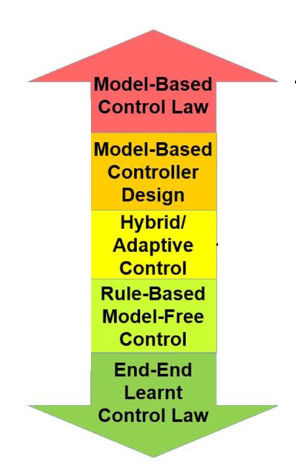
\includegraphics[width=0.2\textwidth]{img02.png}
	\captionsetup{width=0.6\linewidth}
	\caption{The continuum in the literature in regards to control
		methodology ranging from model-based to end-end data-driven
		control \cite{thakar2023survey}}
	\label{fig:img02}
\end{figure}


\textbf{\textit{Mobile Manipulator for Autonomous Localization,
		Grasping and Precise Placement of Construction
		Material in a Semi-Structured Environment}} \quad
A starting point for mobile manipulation is the work \cite{loianno2021construction},
presenting the winning mobile manipulation system for the \textit{Mohamed
	Bin Zayed International Robotics Challenge (MBZIRC)} held in 2020. The proposed system
is comprised of a mobile wheeled base performing localization and navigation in a
semi-structured environment, and a 5-DoF manipulator for grasping and precise placement
of bricks in a carrier. This work was among the first to demonstrate the potentialities
in mobile manipulation in a practical scenario.

%add img13 from the paper
\begin{figure}[H]
	\centering
	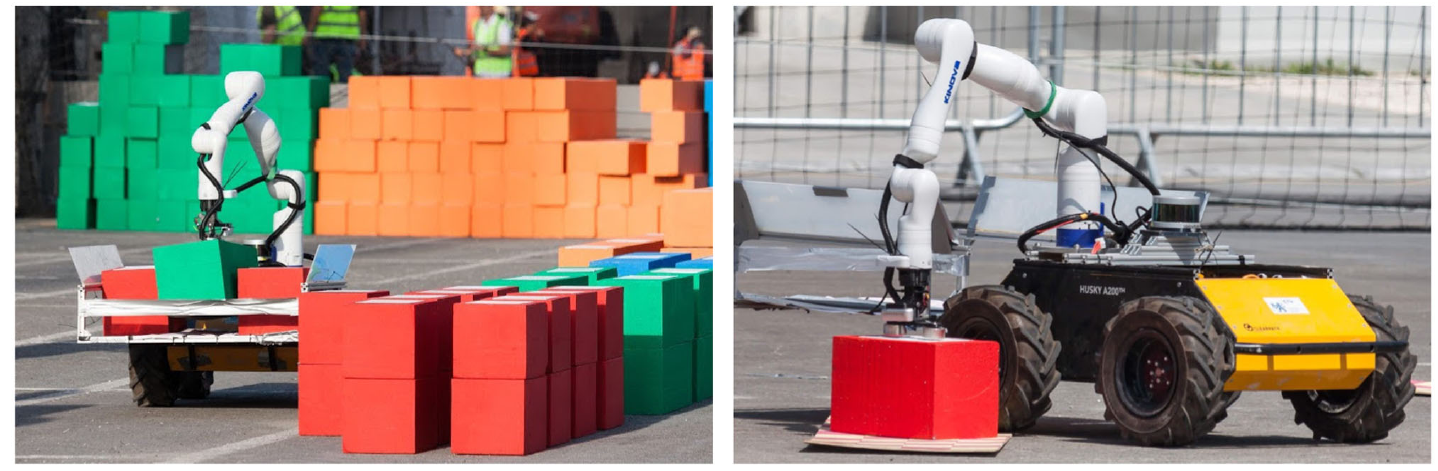
\includegraphics[width=1\textwidth]{img13.png}
	\captionsetup{width=1\linewidth}
	\caption{The described system loading and placing building material
		during the MBZIRC 2020 contest.	\cite{loianno2021construction}}
	\label{fig:img13}
\end{figure}

However, their approach is based on many simplyfying assumptions which may be suitable as a
first one of a kind robotic pick and place system in a real-world scenario and application,
but is not robust enough for a more complex task. For example, the grasping pipeline
is trained to handle only bricks, i.e. solid parallelepiped objects, for which the grasping pose
is straightforward to compute. Furthermore, the robot is not able to autonomously decide
where to place the brick, but it is only able to place it in the predefined position.
Also the arm controller is quite primitive, since it doesn't handle the self collisions
appropriately, and the arm is not able to avoid obstacles in its workspace.

\textbf{\textit{Go Fetch: Mobile Manipulation in Unstructured Environments}} \quad
This work \cite{blomqvist2020gofetch} presents a mobile manipulation system
that combines perception, localization, navigation,
motion planning and grasping skills into one common workflow
for fetch and carry applications in unstructured indoor environments. 
The integration across the various modules is experimentally demonstrated 
in the video \cite{youtube2020gofetch} on the task of finding a commonly available 
object in an office environment, grasping it, 
and delivering it to a desired drop-off location. 

%add img16 from the paper
\begin{figure}[H]
	\centering
	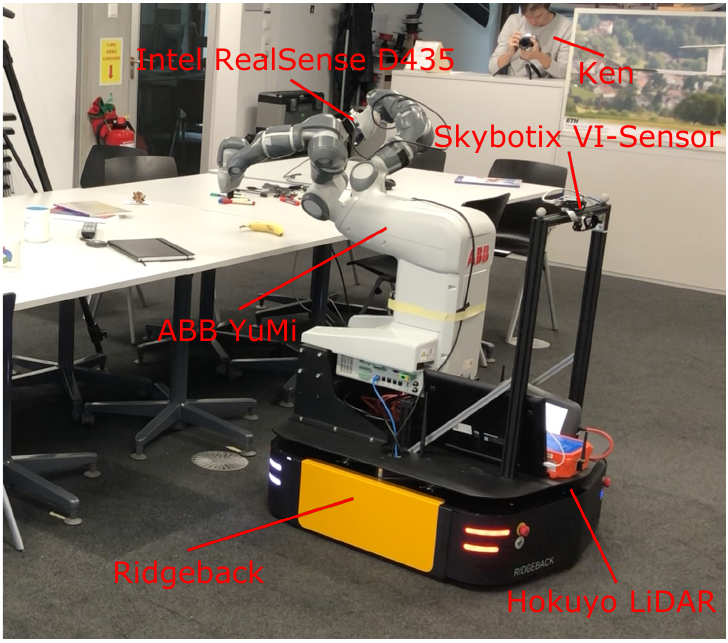
\includegraphics[width=0.6\textwidth]{img16.png}
	\captionsetup{width=0.8\linewidth}
	\caption{A picture of RoyalYumi in action. It features a two-arm ABB Yumi, a Clearpath 
	Ridgeback mobile base, two Hokuyo 2D LiDARs, an	Intel RealSense D435 and a Skybotix VI-Sensor.
	\cite{blomqvist2020gofetch}}
	\label{fig:img16}
\end{figure}

The research \cite{blomqvist2020gofetch} is an example of a mobile manipulation system
for pick and place task in an indoor environment that adopted many simplifications in order
to achieve the desired results. The system uses a series of heuristics to perform the
approaching to the object and the grasping phase, as it can be seen from the demonstration video
\cite{youtube2020gofetch}. The navigation uses a feature-based map and localization
modules, while the arm controller is handled by MoveIt! \cite{moveit2} solver coupled with
the ROS framework \cite{ros2}. This system is not very
well integrated as each phase of the task is carried out by a different module, and shows
how slow and inefficient the robot is in picking the banana. The grasping phase uses multiple
views of the object in order to compute a better grasp pose, which works well
but seems to be overly complex given the predefined task. Overall, the system 
can be regarded as a starting point for mobile manipulation and one of the first
works in dual-arm manipulability.

\subsection{Deep Reinforcement Learning - Data Driven Approach}

Explicit programming is often needed in practice to account for uncertainties in the environment and
sensors used, as well as to solve highly variable problems in an efficient way.
Explicit behavior programming is therefore often tedious and impractical, and more flexible solutions
are needed in environments where the robot must adapt to.
Alternatively, data-driven approaches address the main limitations of traditional methods and propose
to learn robotic behaviours from real experience, thus alleviating the cost of modelling complex behaviours.
This approach allows them to use deep neural networks to model the uncertainties of the environment,
which leads to a more robust controller compared to traditional ones.
Unlike deep learning (DL), the reinforcement learning (RL) paradigm allows to automatically obtain the
experience needed to learn robotic skills through trial-and-error and allows to learn complex decision-making
policies.

With RL, the explicit modelling of the problem is no longer required since the learnt models are grounded
in real experience. Recently, the combination of DL and RL, also known as Deep Reinforcement Learning (DRL),
has made it possible to tackle complex decision-making problems that were previously unfeasible. It combines
the ability of DL to model very high dimensional data with the ability of RL to model decision-making agents
through trial and error.
In fact, DRL has proven to be the state-of-the-art technology for learning complex
robotic behaviours through the interaction with the environment and solely guided
by a reward signal \cite{liu2021deep}.

While ML-based methods are generally used for offline forecasting, DRL is generally used online in
sequential decision-making problems. In fact, DRL allows to autonomously learn complex control policies
through trial and error and only guided by a reward signal. In the case of robotics, the most common
use case is to use such algorithms to model agents capable of performing continuous control of robots.

DRL has been successfully applied in a wide variety of areas such as robotics, computer vision and gaming.
Taking into account the difficulty of modelling complex decision-making robotic skills, DRL offers
a promising way to take advantage of the experience gathered interacting with the environment to
autonomously learn complex robotic behaviours. In particular, the field of DRL applied to robotics has
recently gained popularity due to the remarkable performance obtained in applications 
with high decision-making and control complexity. 
Applications range from manipulation, to autonomous navigation and locomotion.
\cite{iriondo2023learning}

\begin{figure}[H]
	\centering
	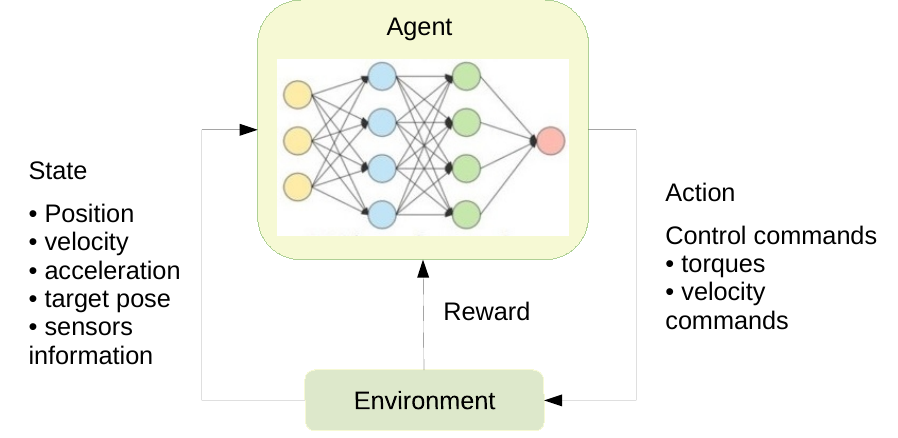
\includegraphics[width=0.7\textwidth]{img03.png}
	\captionsetup{width=0.8\linewidth}
	\caption{A schematic diagram example for robotic manipulation control
		using a data-driven approach such as DRL \cite{liu2021deep}}
	\label{fig:img03}
\end{figure}

\textbf{\textit{Pick and Place Operations in Logistics Using
a Mobile Manipulator Controlled with Deep
Reinforcement Learning}} \quad
The work \cite{iriondo2019pickandplace} presents one of the first and pioneering approaches
to DRL-based methods for pick and place tasks. Their work focused on the positioning
problem, consisting in a local navigation problem where the robot must move to a desired
position moving by small distances in a confined environment to reach the target object.
They relied on DRL for controlling the mobile wheeled base robot, while the arm controller
was handled by MoveIt! framework \cite{moveit2}. This can be regarded as a first step towards
more complex tasks, as it shows the foundations of DRL-based methods for mobile manipulation.
The method had some flaws, like the imprecise navigation due to errors in localization and
odometry, which the network was not able to overcome, since it was not fed video data stream.
However, it paved the wasy for a lot of other works, many of which mentioned in this chapter.

\textbf{\textit{Fully Autonomous Real-World Reinforcement
		Learning with Applications to Mobile Manipulation}} \quad
A work from Berkeley AI research \cite{sun2022relmm} show \textit{ReLMM}, a model that
can learn continuously on a real-world platform without any environment instrumentation,
without human intervention, and without access to privileged information, such as maps,
objects positions, or a global view of the environment. Their method employs a
modularized policy with components for manipulation and navigation, where manipulation
policy uncertainty drives exploration for the navigation controller, and the manipulation
module provides rewards for navigation. They trained the policy on a room cleanup task, where
the robot must navigate to and pick up items scattered on the floor.
The robot learns entirely from its own sensors in a real-world environment, without any
simulation and minimal human intervention. Furthermore, the entire learning process is efficient
enough for real-world training. On top of this, the robot is able to continually gather data
at scale and improve its performance over time, with the auto-reset functionality.

%add img11 from the paper
\begin{figure}[H]
	\centering
	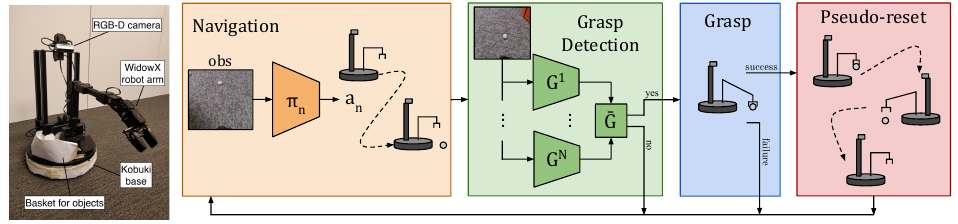
\includegraphics[width=1\textwidth]{img11.png}
	\captionsetup{width=1\linewidth}
	\caption{ReLMM partitions the mobile manipulator into a navigation policy
		and grasping policy. Both policies are rewarded when an object is grasped
		\cite{sun2022relmm}}
	\label{fig:img11}
\end{figure}

Although the results shown in \cite{sun2022relmm} demonstrate efficient performance in
the pick and place task, there are many issues circumvented by simplyfying the problem.
For example, the robot is very small, a modified version of Turtlebot, running in a small and
contained environment. They didn't address any safety and collision issues since the platform
mounted bumping sensors, and any collision would not harm the robot at all. Doing so enabled them
to train the policy online without any prior simulation.
Furthermore the kinematics of the mobile base and the robotic arm are very simple, and having the
stereo camera mounted on top of the robotic platform allowed them to easily detect the objects
on the floor. This work paves the way for more complex systems and tasks, but it is still far
from being a general solution for mobile manipulation.

\subsection{Challenges in Data-Driven approaches}

Two of the most important challenges here concern \textbf{sample efficiency and generalization}.
The goal of DRL in the context of robotic manipulation
control is to train a deep policy neural network, to detect the optimal
sequence of commands for accomplishing the task. The current state of the algorithm can include
the angles of joints of the manipulator, position of the end effector, and their derivative information,
like velocity and acceleration. The output of this policy network is an action indicating control
commands to be implemented to each actuator, such as torques or velocity commands. When the robotic manipulator
accomplishes a task, a positive reward will be generated. With these delayed and weak
signals, the algorithm is expected to find out the most successful control strategy for the
robotic manipulation \cite{liu2021deep}.

The challenges of learning robust and versatile manipulation skills
for robots with DRL are still far from being resolved satisfactorily for real-world application.
Currently, robotic manipulation control with DRL may be suited to fault tolerant
tasks, like picking up and placing objects, where a disaster will not be caused if the
operation fails occasionally. It is quite attractive in situations, where there is enough
variation that the explicit modeling algorithm does not work \cite{liu2021deep}.

However, even in this kind of applications, DRL-based methods are not widely
used in real-world robotic manipulation. The reasons are multiple, including sample efficiency and generation,
where more progress is still required, as both gathering experiences by interacting with
the environment and collecting expert demonstrations for imitation learning are expensive
procedures, especially in situations where robots are heavy, rigid and brittle, and it will
cost too much if the robot is damaged in exploration. Another very important issue is
\textbf{safety guarantee}. Not like simulation tasks, we need to be very careful that learning
algorithms are safe, reliable and predictable in real scenarios, especially if we move to
other applications that require safe and correct behaviors with high confidence, such as
surgery or household robots taking care of the elder or the disabled. There are also other
challenges including but not limited to the algorithm explainability, the learning speed,
high-performance computational equipment requirements. \cite{liu2021deep}

\textbf{\textit{Learning positioning policies for mobile manipulation operations
		with deep reinforcement learning}}
\quad
The work proposed in \cite{iriondo2023learning} is a practical example of a DRL-based approach
facing these challenges and the enormous limitations to overcome (as well as the potentialities).
The mobile platform in figure \ref{fig:img01} is used in an industrial environment for an
approaching task. The robot learns to navigate itself to the desk where the target object is located,
then uses the MoveIt! planner to check whether the trajectory to pick the object is feasible.
The robot locates itself using AMCL and the learned policy serves as a controller for
local navigation task. Their work show many shortcomings of this approach, such as the
difficult integration between the DRL policy and localization package, with noise in the
real environment affecting negatively the performance of the robot. As a result,
the video presented shows an inefficient an jiggly movement
because of the non-smooth control policy. In fact, they mention the necessity of mounting
a stereo camera for navigation, in order to reduce the errors in the localization and
improve the navigation of the robot.


\begin{figure}[H]
	\centering
	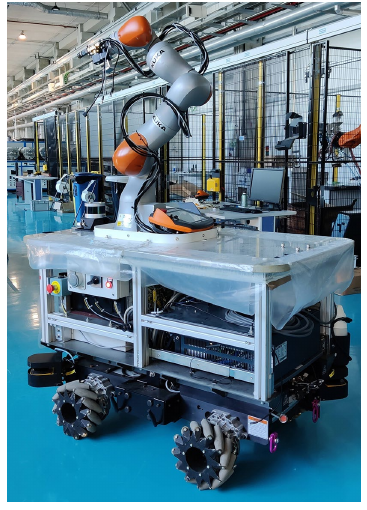
\includegraphics[width=0.5\textwidth]{img01.png}
	\captionsetup{width=0.6\linewidth}
	\caption{KUKA robot mounted on a mobile platform for pick and place tasks
		in industrial environments \cite{iriondo2023learning}}
	\label{fig:img01}
\end{figure}



\textbf{\textit{Deep Reinforcement Learning Based Mobile Robot Navigation Using Sensor Fusion}} \quad
The problem of unstable and imprecise navigation with learned policies is overcome in the
paper \cite{yan2023drlnavigation}, which proposes a DRL-based approach for navigation in dynamic
environments. The proposed method is based on the Deep Deterministic Policy Gradient (DDPG)
algorithm, which is a model-free, off-policy actor-critic algorithm that uses deep neural networks
to represent the policy and the critic functions. The proposed method is evaluated in a
simlated environment where the robot learns to navigate effectively and smoothly, while avoiding
unknown dynamic obstacles. This work shows the right direction towards more robust
navigation and obstacle avoidance systems.

\section{Whole-body mobile manipulator control}

In most control approaches to mobile manipulation, base and manipulator operation are strictly
separated such that at any given time only one primary control objective is
active. This separation principle is then augmented by a switching layer that determines the
currently pertinent control objectives. The advantage of such a control formulation lies in its
implicity, i.e., priorities can be separated among the arm and the base with individually
designed different control algorithms employed for each subsystem \cite{thakar2023survey}.

Instead, we refer to \textbf{whole-body control} as a unified control framework that considers
the mobile manipulator as a single system (arm manipulator mounted on a mobile wheeled/legged robot).
Despite the disadvantage that unified control needs to adhere to a single control framework,
it allows for the exploitation of mobile manipulation in the true sense of the term,
wherein the manipulator and mobile base can be controlled at the same time. This can lead
to several advantages during task achievement and makes the robot more dynamic in terms
of its capabilities. The formulation for this type of control involves considering
the onboard manipulator as an extended joint space of the mobile base, where the motion controller
considers both the base and manipulator state. As a result, base control can be completed
simultaneously without affecting much the performance of the end-effector manipulability
\cite{thakar2023survey}.

\subsection{MPC+IK for articulated object manipulation}

\textbf{\textit{Articulated Object Interaction in Unknown Scenes
		with Whole-Body Mobile Manipulation}} \quad
In a work conducted in universities in Zurich and Toronto \cite{mittal2022articulated},
the researchers demonstrated a successful application of whole-body control for a mobile
manipulator. The proposed system introduces a two-stage architecture for autonomous interaction
with large articulated objects in unknown environments.

%add image from the paper
\begin{figure}[H]
	\centering
	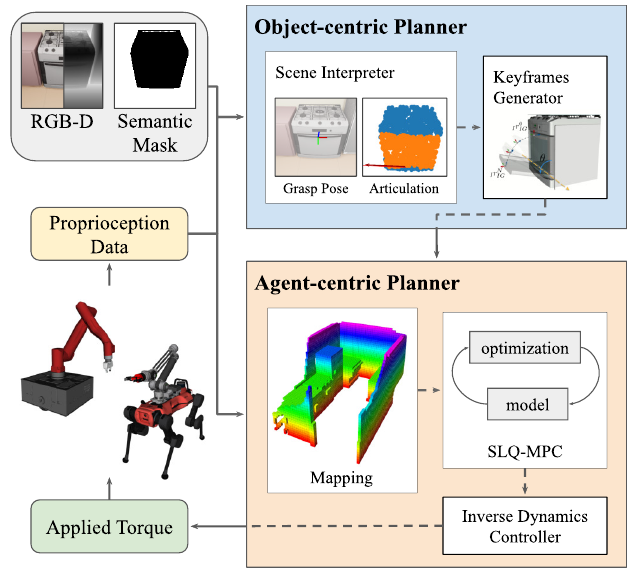
\includegraphics[width=0.7\textwidth]{img04.png}
	\captionsetup{width=0.9\linewidth}
	\caption{ The two-level hierarchy in the proposed framework. The
		object-centric planner comprises of a scene interpreter and keyframe
		generator. It uses perceptual information to generate task space
		plans. The agent-centric planner follows the computed plan while
		satisfying constraints and performing online collision avoidance.
		\cite{mittal2022articulated}}
	\label{fig:img04}
\end{figure}


In the first stage, an object-centric planner focuses solely on the object, providing an
action-conditional sequence of states for manipulation using RGB-D data.
The second stage involves an agent-centric planner that formulates whole-body motion control
as an optimal control problem, ensuring safe tracking of the generated plan, even in scenes
with moving obstacles.
The system proposed in \cite{mittal2022articulated} demonstrates effectiveness in handling complex static and
dynamic kitchen settings for both wheel-based and legged mobile manipulators. A comparison with
other agent-centric planners reveals a higher success rate and lower execution time. Hardware
tests on a legged mobile manipulator further confirm the system's capability to interact with
various articulated objects in a real kitchen. The approach combines object-centric and
agent-centric planning, leveraging MPC-based solutions for improved success rates and reduced
execution times, particularly in articulated object manipulation scenarios. The contributions
include the extension of collision-free whole-body MPC for mobile manipulation, benchmarking
in hyper-realistic simulation, and successful hardware experiments showcasing the system's
real-world applicability.


%add image from the paper
\begin{figure}[H]
	\centering
	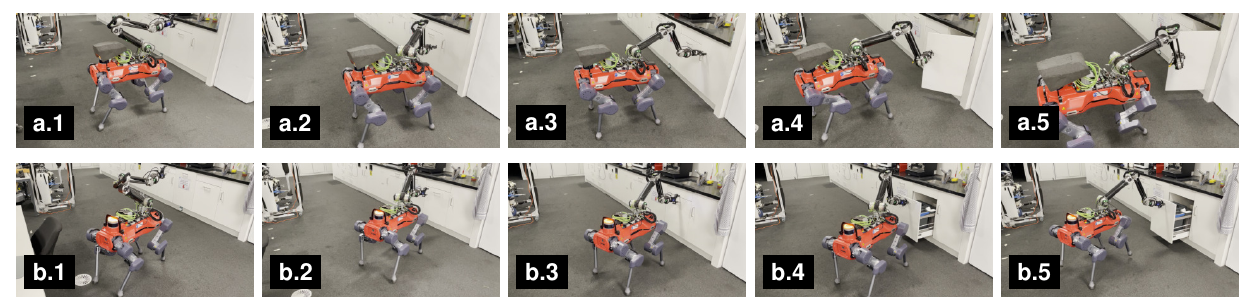
\includegraphics[width=1\textwidth]{img05.png}
	\captionsetup{width=1\linewidth}
	\caption{Legged mobile manipulation of articulated objects in the kitchen test scenario:
		(a) Drawer, (b) Cabinet. Throughout the interaction, we set the robot gait schedule
		to trot. Only while grasping the handle, the robot enters stance mode.
		\cite{mittal2022articulated}}
	\label{fig:img05}
\end{figure}


The work \cite{mittal2022articulated}, published in 2022, is the first and one of a kind
in successful real-world application of whole-body control using a MPC-based approach
combined with IK solvers for articulated object manipulation.
Furthermore, they achieved good performance in both dynamic
and static real world environments, which is a very challenging task for most of the
existing methods. However, the proposed method is limited mostly with respect to the grasping
capabilitities, which were hard-coded into the known interactive objects (in their case,
the kitchen appliances handles), meaning that explicit behavior programming and tuning was
needed for the grasping task. They propose data-centric methods to overcome these limitations.
This research proved the feasibility of this approach, which many other researchers claimed
to be unfeasible and way too complex to be implemented in real-world applications. However,
it is worth noting that the proposed method is not a general solution for all robots hardware
configurations, and extending it to other robots would require a lot of effort and time,
since it boils down to an optimal control problem.

\subsection{Deep Reinforcement Learning for high DoF control}

\textbf{\textit{Deep Whole-Body Control: Learning a Unified Policy
		for Manipulation and Locomotion}} \quad
The research paper \cite{fu2022deeplegged} addresses the challenges in controlling legged
manipulators with attached arms, proposing a novel approach to learn a unified policy for
whole-body control using deep reinforcement learning. The standard hierarchical control pipeline
is critiqued for its inefficiency, requiring significant engineering to coordinate
arm and leg movements. The proposed method, Regularized Online Adaptation, aims to bridge the Sim2Real gap,
and Advantage Mixing is introduced to overcome local minima during training.
The authors present a low-cost legged manipulator design and demonstrate that their
unified policy enables dynamic and agile behaviors across various tasks.

%add image from the paper
\begin{figure}[H]
	\centering
	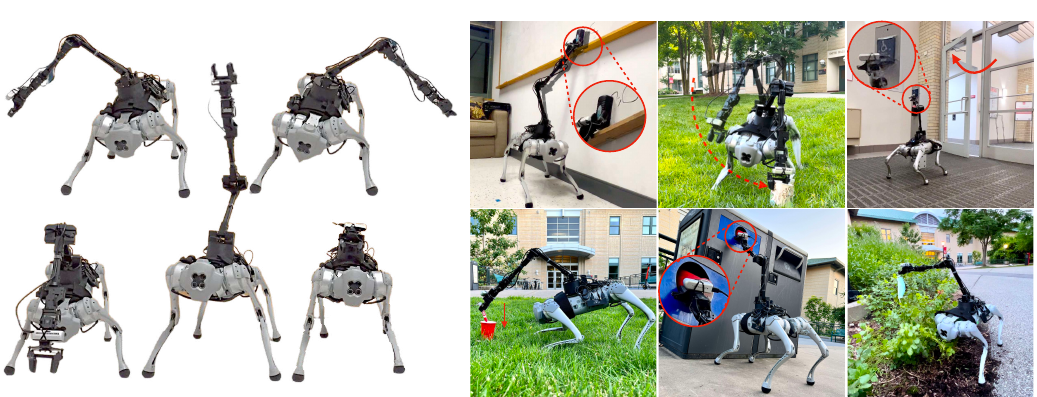
\includegraphics[width=1\textwidth]{img06.png}
	\captionsetup{width=1\linewidth}
	\caption{Framework for whole-body control of a legged robot with a robot arm attached.
		Left half shows how whole-body control achieves larger workspace by leg bending and stretching.
		Right half shows different real-world tasks, including wiping whiteboard, picking up a cup,
		pressing door-open buttons, placing, throwing a cup into a garbage bin and picking
		in clustered environments. \cite{fu2022deeplegged}}
	\label{fig:img06}
\end{figure}

The paper emphasizes the limitations of current hierarchical models, advocating for learning-based
methods like reinforcement learning to reduce engineering efforts and improve generalization.
However, it critiques existing learning-based approaches for semi-coupling legs and arms,
highlighting issues of coordination, error propagation, and non-smooth motions.
The proposed unified policy not only allows coordination but also enhances the capabilities
of individual components, such as the robot dynamically adjusting leg movements to extend
the arm's reach \cite{fu2022deeplegged}.

The challenges in scaling standard sim2real reinforcement learning to whole-body control
are discussed, including the high degree of freedom, conflicting objectives, and dependencies
between manipulation and locomotion. The paper introduces a hardware setup for a low-cost, fully
untethered legged manipulator and outlines a method for learning a unified policy to control
both legs and the arm. The authors leverage causal structure in action space and regularization
for domain adaptation to enhance stability and speed up learning.
The proposed method is evaluated through tasks like teleoperation and vision-guided tracking,
demonstrating successful picking tasks using visual feedback from an RGB camera.
Comparative analysis with a baseline method (MPC+IK) across various pick-up tasks measures success rate,
average time to completion, IK failure rate, and self-collision rate.
The authors conclude by acknowledging the preliminary nature of their results and highlight
potential extensions, such as incorporating vision-based policies and addressing challenges
in general-purpose object interaction \cite{fu2022deeplegged}.

%add image from the paper
\begin{figure}[H]
	\centering
	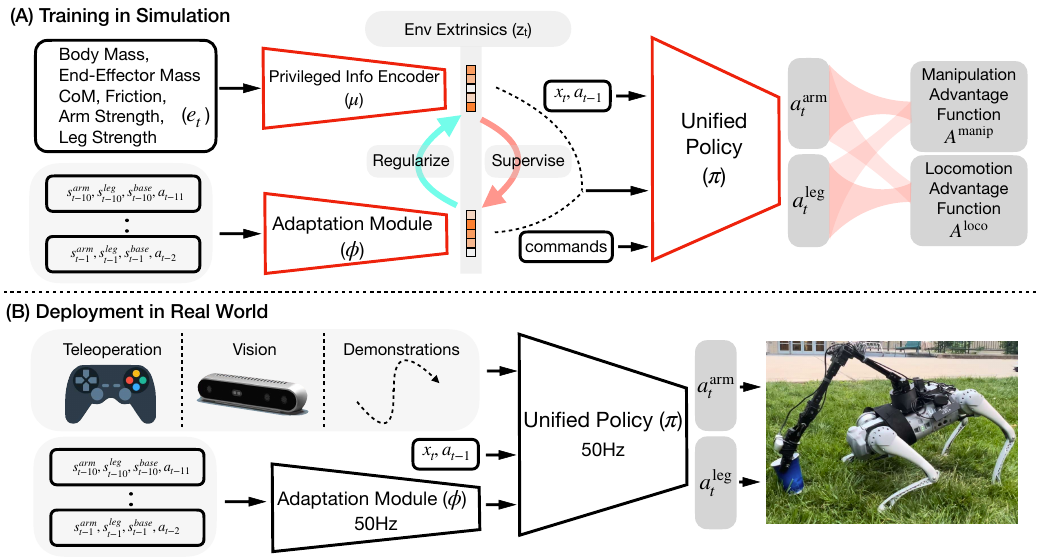
\includegraphics[width=1\textwidth]{img07.png}
	\captionsetup{width=1\linewidth}
	\caption{Whole-body control framework. During training, a unified policy is learned by conditioned on
		environment extrinsics. During deployment, the adaptation module is reused without
		any real-world fine-tuning.
		The robot can be commanded in various modes including teleoperation, vision and demonstration replay.
		\cite{fu2022deeplegged}}
	\label{fig:img07}
\end{figure}

As the authors of the paper \cite{fu2022deeplegged} state, the main limitation (but also the core
idea behind the control input) is the fact that the robot requires a human operator to
provide the robot objectives, which are then translated into the control inputs. In fact,
the robot is not able to autonomously decide what to do, but it is only able to either track the
end effector pose given by the human operator, or to track the April marker in the human's hand.
This limitation can be overcome with appropriate task training, but it is not a general solution.
However, the proposed method is very promising, since it is able to achieve very good results
in the robot body-hand coordination, which is a very challenging task for most of the existing
methods. The movements look very smooth and natural, and the robot is able to perform
simple task in dynamic environment. The April marker tracking mode shows also the effectiveness of
the use of a stereo camera for tracking the objective, meaning that promising results can be
achieved in other tasks. This research used Isaac Gym as a simulation environment, which
proved to be very powerful for training and overcoming the simulation-to-reality gap.

\textbf{\textit{Learning Mobile Manipulation through Deep
		Reinforcement Learning}} \quad
\cite{wang2020drlmanipulation}
This paper presents a pioneering mobile manipulation system that leverages deep
reinforcement learning for unstructured environments. It uniquely integrates state-of-the-art
algorithms with visual perception, adopting an efficient framework that separates
visual processing from control. This design enables seamless generalization from simulation
training to real-world scenarios, utilizing only on-board sensors.
Notably, the transferability of policies from simulation to real robots is a key strength,
demonstrating the system's autonomy in grasping diverse objects across varied scenarios.
The evaluation centers around a challenging mobile picking task, encompassing object recognition,
collision-free robot-arm control, and object picking based on the learned policy.


%add img14 from the paper
\begin{figure}[H]
	\centering
	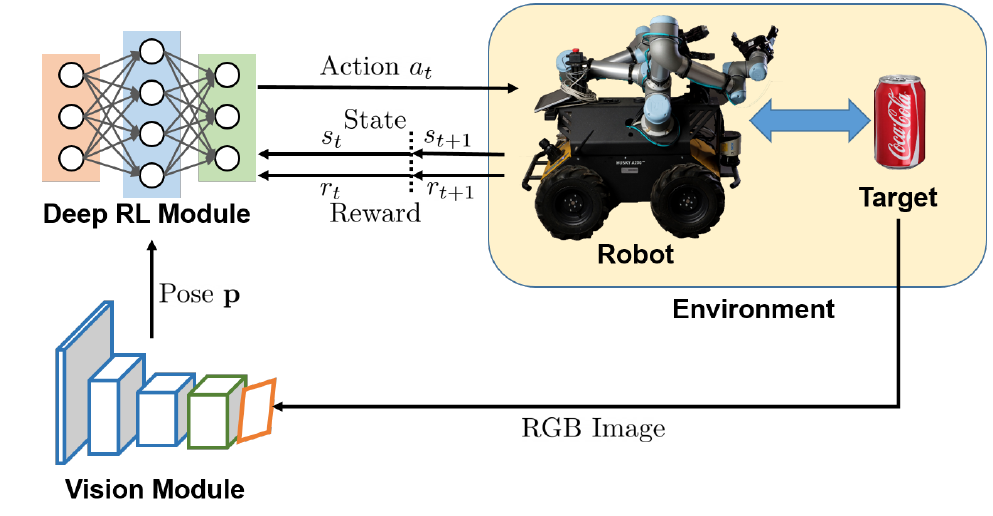
\includegraphics[width=1\textwidth]{img14.png}
	\captionsetup{width=1\linewidth}
	\caption{Learning-based mobile manipulation control framework. There are mainly two parts,
		deep reinforcement learning module and vision module. First, the vision module estimates
		the object 6-degrees of freedom pose $p$ from images captured by an on-board RGB stereo camera.
		Then, based on the object pose $p$ and current robot state st, deep reinforcement learning
		module predicts an action at for the robot to act. A new state $s_{t+1}$ and a reward
		$r_{t+1}$ are received after action.\cite{wang2020drlmanipulation}}
	\label{fig:img14}
\end{figure}

Comparative assessments with state-of-the-art reinforcement learning algorithms highlight
the stability and efficacy of the Proximal Policy Optimization (PPO) based system.
Real-world experiments further confirm the system's ability to autonomously execute mobile grasping,
overcoming challenges posed by the intricate nature of mobile base, arm, gripper, and vision subsystems.
Acknowledging differences between simulation and real-world dynamics, the paper addresses
the need for closer coupling between mobile base and arm motions in future work. Overall,
this work represents a significant contribution to the field, showcasing the potential of
deep reinforcement learning for autonomous mobile manipulation in complex, unstructured environments.

%add img15 from the paper
\begin{figure}[H]
	\centering
	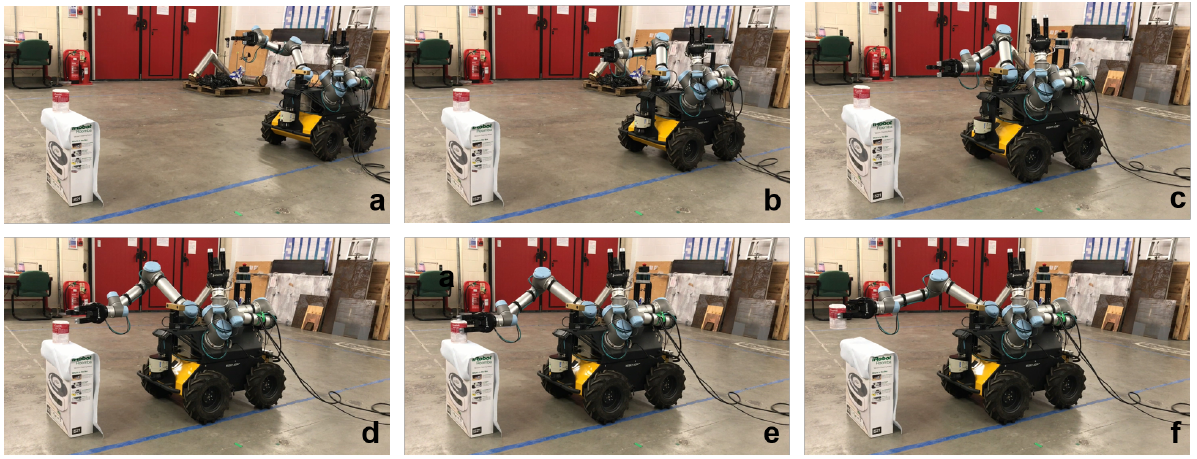
\includegraphics[width=1\textwidth]{img15.png}
	\captionsetup{width=1\linewidth}
	\caption{Real mobile grasping process for a soup can.
	(a) is starting, (b,c,d) is approaching, (e) is grasping, (f) is picking up.
	\cite{wang2020drlmanipulation}}
	\label{fig:img15}
\end{figure}

The method proposed in \cite{wang2020drlmanipulation} is very promising, since it is able to
achieve very good results in the robot body-hand coordination, which is a very challenging task
especially in dynamic environments. The movements look very smooth and natural, and the robot is
able to perform simple task in dynamic environment. This approach is one of the first able
to achieve such complex control using vision-based perception together with deep reinforcement
learning. However, it is far from being an optimal solution, since it achieves simple
tasks in a very controlled environment. The research paper mentioned below is from the same
research group, demonstrating the new advancements in their research.

\textbf{\textit{Multi-Task Reinforcement Learning based Mobile Manipulation 
	Control for Dynamic Object Tracking and Grasping}} \quad
This research paper \cite{wang2022multitask} is a continuation of work demonstrated in the
their previous research paper \cite{wang2020drlmanipulation} mentioned above.
\cite{wang2022multitask} addresses the challenges associated with
agile control of mobile manipulators in unstructured environments, particularly focusing
on dynamic object tracking and grasping. The authors propose a multi-task reinforcement
learning-based control framework that aims to achieve general dynamic object tracking and
grasping capabilities. The framework utilizes various dynamic trajectories as a training set,
incorporating random noise and dynamics randomization to enhance policy generalization.
Experimental results demonstrate the trained policy's ability to adapt to unseen dynamic
trajectories, achieving a 0.1m tracking error and a 75\% grasping success rate for dynamic objects.
The proposed method is successfully deployed on a real mobile manipulator, showcasing its
potential for real-world applications. The contributions of this work include the development
of a versatile control framework and its successful deployment in unstructured environments,
addressing the challenges of mobile manipulation with dynamic objects.

%add image from the paper
\begin{figure}[H]
	\centering
	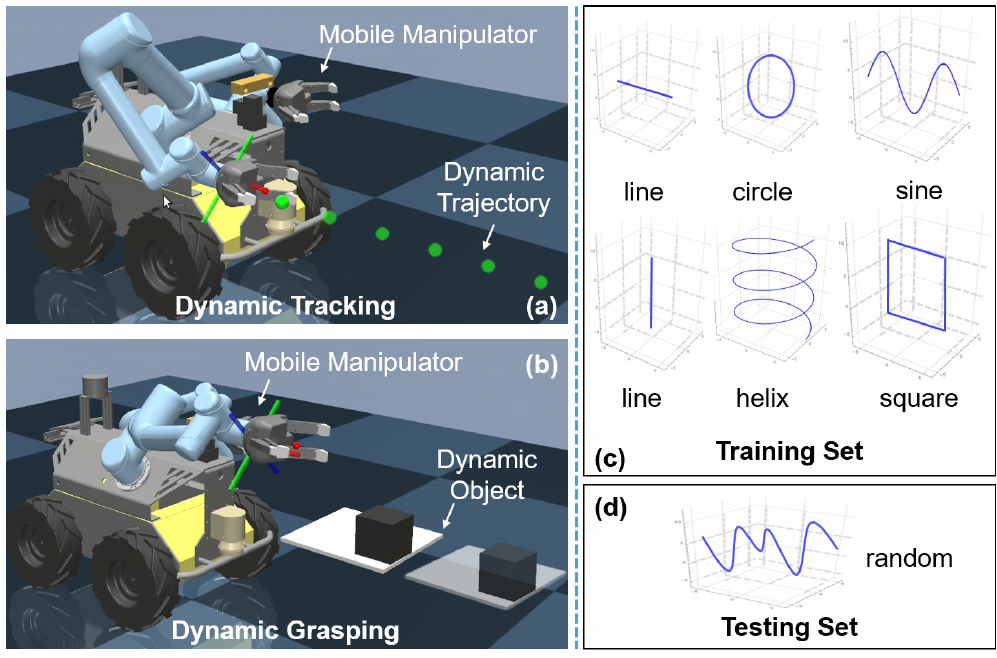
\includegraphics[width=1\textwidth]{img08.png}
	\captionsetup{width=1\linewidth}
	\caption{(a) Dynamic trajectory tracking task with a mobile manipulator. (b)
		Dynamic object grasping task with a mobile manipulator. (c) Several basic
		trajectories as multi-task RL training set. (d) Random trajectories as multi-task
		RL testing set.\cite{wang2022multitask}}
	\label{fig:img08}
\end{figure}

In \cite{wang2022multitask} they use the proximal policy optimization (PPO) algorithm to train
and learn a policy, but the method is general and can be applied to most on/off-policy RL algorithms.
PPO is one of the state-of-the-art RL algorithms that is easy to implement and tune, and performs
relatively well. The policy is learned through a deep neural network.

%add image from the paper
\begin{figure}[H]
	\centering
	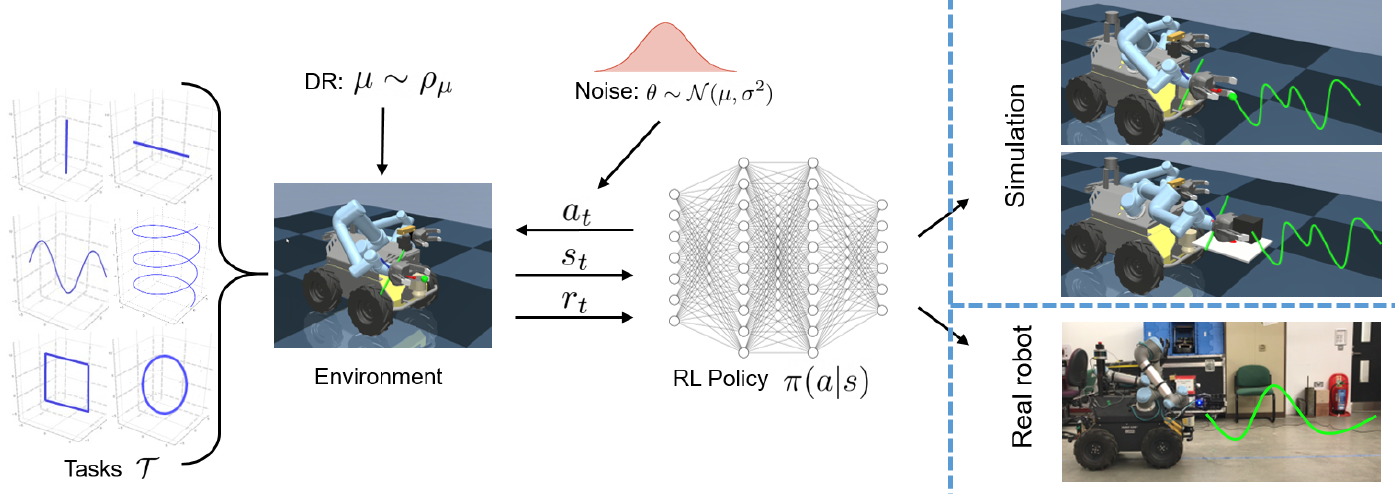
\includegraphics[width=1\textwidth]{img09.png}
	\captionsetup{width=1\linewidth}
	\caption{(a) In the multi-task RL training, six basic trajectories are used as the task
		training set to train a general policy. To improve the robustness, gaussian noise is added
		to the action and observation space in each training episode. (b) The RL testing includes
		simulation and real world for policy evaluation.\cite{wang2022multitask}}
	\label{fig:img09}
\end{figure}

The images above show the training and testing process of the proposed method. They created a
realistic simulation environment which enabled efficient parallel training of the policy,
and simulation of the dynamic objects and tracking. They also managed to correctly transfer the
learned policy to the real robot, which is a very challenging task for most of the existing methods.
Artificial noise addition was essential for the training process, since it allowed the policy
to generalize better to unseen trajectories and environments.

%add image from the paper
\begin{figure}[H]
	\centering
	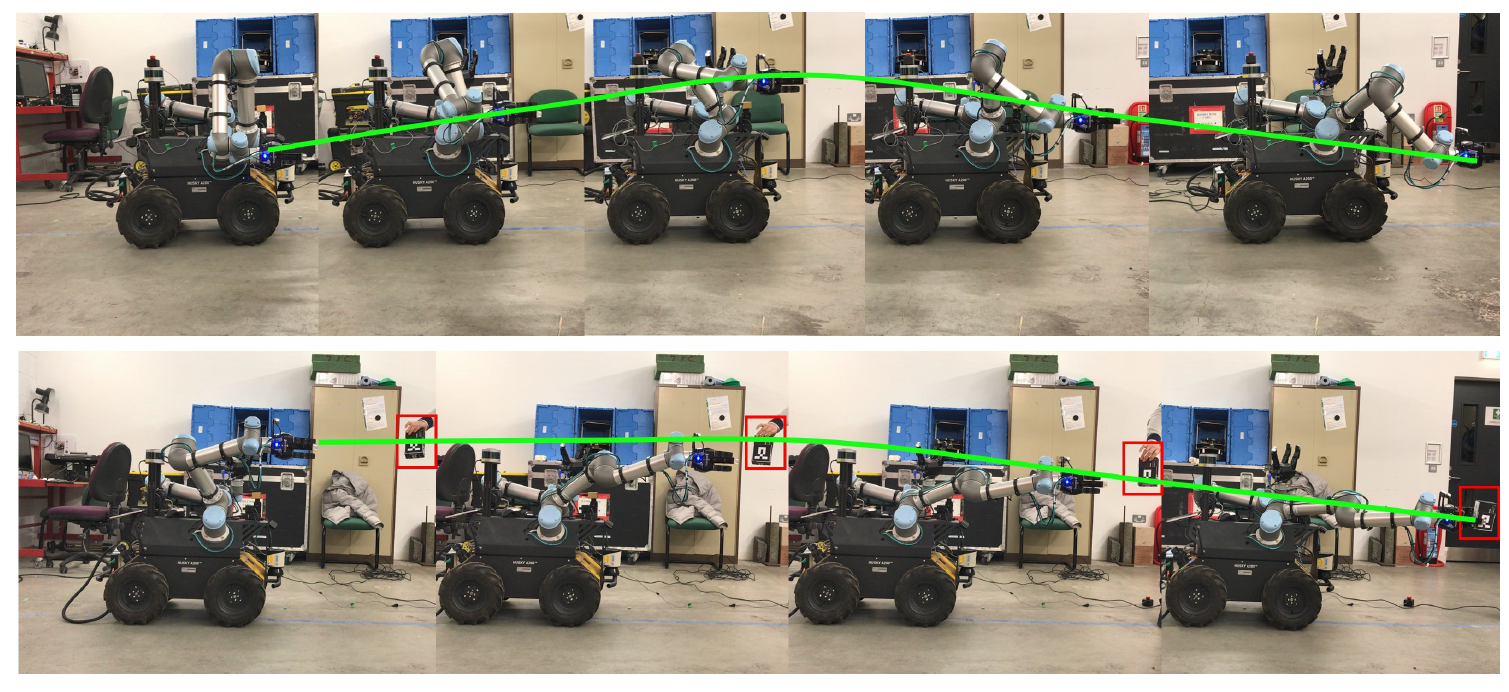
\includegraphics[width=1\textwidth]{img10.png}
	\captionsetup{width=1\linewidth}
	\caption{Snapshots of the real robot experiments. The upper row shows a mobile
		tracking process in which the end-effector try to track the target trajectory.
		The lower row shows a mobile grasping process in which the object moves
		randomly. \cite{wang2022multitask}}
	\label{fig:img10}
\end{figure}

Overall, this research provides valuable insights and a practical solution for advancing the
field of agile mobile manipulation. This is one of the very few works that addresses the
problem of dynamic object tracking and grasping, which is a very challenging task for most
of the existing models, due to the difficulty in modeling and the extensive training required. Although
the model doesn't show very high success rate in the tasks shown, it shows promising results
and a direction of research that can be further explored.



\subsection{Comparison of Model-Based and Data-Driven approaches}


\singlespacing
\begin{table}[H]
	\centering
	\begin{tabular}[c]{|m{3cm} || m{6cm} | m{6cm}|}
		\hline
		\raggedleft \textbf{Approach}                           &
		\textbf{Model-Based}                                    &
		\textbf{Data-Driven}
		\\
		\hline \hline

		\raggedleft \textbf{Control Strategies}                 &
		\customtablelist{
			\item Model Predictive Controllers (MPC)
			\item Whole-Body Inverse Kinematics (IK) Solver
		}                                                       &
		\customtablelist{
			\item Deep Reinforcement Learning (DRL)
			\item Imitation Learning
		}
		\\
		\hline

		\raggedleft \textbf{Features}                           &
		\customtablelist{
			\item Requires explicit modeling of system dynamics and kinematics
			\item Suitable for simple tasks, unsuitable for complex tasks
			\item Planning over end-effector pose or grasp in the workspace
		}                                                       &
		\customtablelist{
			\item No explicit modeling of system dynamics
			\item Learning from experience in simulation environments
			\item High-level planning over tasks, object detection, manipulation
			or other objectives
		}
		\\
		\hline

		\raggedleft \textbf{Interpret-ability and Adaptability} &
		\customtablelist{
			\item Explitic modeling implies high system interpretability
			\item Adaptable to many tasks but requires behaviors re-programming
		}                                                       &
		\customtablelist{
			\item Learned policies have very limited interpretability
			\item Learning from experience allows high adaptability,
			given proper GPU-parallelized training
		}                                                         \\
		\hline

		\raggedleft \textbf{Advantages}                         &
		\customtablelist{
			\item Small simulation-to-reality gap
			\item Adaptable to many tasks but with explicit programming
			\item No training required
			\item Safer operation due to explicit physical limitations modeling
		}                                                       &
		\customtablelist{
			\item No explicit modeling of system dynamics required
			\item Learning from experience allows high generalization
			\item Can perform well in unknown or dynamic environments
			\item Can provide high body-hand movement coordination
		}                                                         \\
		\hline

		\raggedleft \textbf{Disadvantages}                      &
		\customtablelist{
			\item Requires very accurate physical models for seamless integration
			\item Doesn't perform well in complex tasks or dynamic environments
			\item Difficult to adapt to complex tasks (low generalization)
			\item High computational cost for the solver in high DoF systems
		}                                                       &
		\customtablelist{
			\item Requires large amounts of training data and extensive training
			\item Very long time needed to fine tune the hyperparameters
			\item May result in unstable and jiggly movements
			\item May result in unsafe behaviors in real-world applications
			if not properly trained
			\item Suffers a lot from the simulation-to-reality gap
		}                                                         \\
		\hline
	\end{tabular}
	\caption{Summary of the main differences between model-based and data-driven approaches
		for robotic manipulator controls}
	\label{table:1}
\end{table}

\onehalfspacing


\section{Addressing the Simulation-to-Reality Gap}

\textbf{\textit{A Sim-to-Real Pipeline for Deep Reinforcement
		Learning for Autonomous Robot Navigation in
		Cluttered Rough Terrain}} \quad
A work from Toronto \cite{zhang2021simtoreal} proposes a sim-to-real pipeline for
deep reinforcement learning for autonomous robot navigation in cluttered rough terrain.
Sim-to-real strategies have been developed for robot navigation tasks. For example,
domain randomization can be applied to visual parameters such as texture,
lighting, and object placement in synthetic environments to improve the generalizability.
The paper \cite{zhang2021simtoreal} addresses the "sim-to-real Gap" in training robots for
3D terrain navigation by incorporating three sim-to-real strategies. Firstly, to account
for depth camera measurement errors in 3D mapping that affect terrain steepness accuracy,
the authors vary terrain steepness during training using a uniform distribution.
Secondly, the paper tackles disturbances in robot motion during interactions with rough
terrain, such as slippage and insufficient traction. Both 3D terrain interactions and
latency from visual odometry measurements contribute to disturbances in robot travel distance
and yaw rotation angle. The third strategy focuses on addressing robot pose estimation errors
arising from image and feature association errors. These errors, caused by lens distortion
and ambiguous features, impact the accuracy of the robot's estimated 6 DOF pose.
The paper integrates these errors into the inputs of the DRL network to improve the
model's performance in the face of localization inaccuracies.



\section{Object Detection and Grasping}

Grasp planning for mobile manipulators is a challenging problem that has been
dealt with in several ways in the literature. On the one hand, grasping requires coordination
within a very challenging high-dimensional constrained configuration space (mobile base /
manipulator / gripper). Further, grasping requires detecting object, constructing data-driven
representation, determining the gripper approach-vector, and computing all the mobile manipulator's
plans in the presence of uncertainty. Many of the traditional grasp planners (designed for stationary
manipulators) can be used for mobile manipulators once the mobile base has been fixed.
However, a generic grasping pipeline is desirable, which achieves arm-base-gripper
coordinated grasping given the information about object pose and
the operating environment. Such concurrent manipulator / mobile base motion approaches are being
explored till grasping is successful or at least until the gripper reaches the
objects (and only manipulator moves for grasping). This may not be optimal as grasping can happen
with the mobile base and the manipulator moving when the gripper is closing \cite{thakar2023survey}.

Broadly, automated grasping can be categorized into the following approaches 
\cite{asadi2019construction}: 

\begin{enumerate}
	\item grasp using prior information from scene/objects
	\item grasp using hand-eye coordination through learning directly from raw sensor data
	\item grasp using template matching
	\item grasp by detecting proper grasping pose using deep learning-based approaches
	\item other field-specific approaches
\end{enumerate}

Systems in each category have one or more limitations that are detailed in the following
subsections. The majority of the existing systems are static, where a robotic system 
is fixed in an environment surrounded by the objects in its workspace.

\textbf{\textit{Automated Object Manipulation Using Vision-Based Mobile 
Robotic System for Construction Applications}} \quad
The system designed and deployed for pick-and-place in a structured construction environment
\cite{asadi2019construction} integrates scene understanding and autonomous navigation 
with object grasping. To achieve this, two stereo cameras and a robotic arm are mounted
on a mobile platform. This integrated system uses a global-to-local control planning strategy
to reach the objects of interest (in this study, bricks, wood sticks, and pipes). 
Then, the scene perception, together with grasp and control planning, enables the system
to detect the objects of interest, pick, and place them in a predetermined location depending
on the application.
The system is implemented and validated in a construction-like environment for pick-and-place
activities. The results demonstrate the effectiveness of this fully autonomous system 
using solely onboard sensing for real-time applications with end-effector positioning
accuracy of less than a centimeter.
However, the researchers mention also the shortcomings of the system, since the robot
was developed for a field-specific application, therefore non-adaptable to more generic
use case scenarios. The system uses a heuristic-based approach in order to detect the
bricks to grasp and pick up. Furthermore, the navigation pipeline relies on a static environment
with no dynamic obstacles, since the arm manipulator does not employ any collision avoidance
in the trajectory planning \cite{asadi2019construction}.


\textbf{\textit{Autonomous Robotic Manipulation: Real-Time, Deep-Learning
		Approach for Grasping of Unknown Objects}} \quad
The work \cite{sayour2022unknowngrasping} proposes a novel approach for grasping unknown objects.
The researhers present a full grasping pipeline proposing a real-time data-driven
deep-learning approach for robotic grasping of unknown objects using MATLAB and
deep convolutional neural networks. The proposed approach employs RGB-D image data
acquired from an eye-in-hand camera centering the object of interest in the field of
view using visual servoing. Their approach aims at reducing propagation errors
and eliminating the need for complex hand tracking algorithm, image segmentation,
or 3D reconstruction, which are often either infeasible or too prone to errors.
The proposed approach is able to efficiently generate reliable multi-view object grasps
regardless of the geometric complexity and physical properties of the object in question.
The system employed is a 7 DoF robotic manipulator controlled with an IK solver,
and a parallel gripper with overactuated fingers.

%add img12 from the paper
\begin{figure}[H]
	\centering
	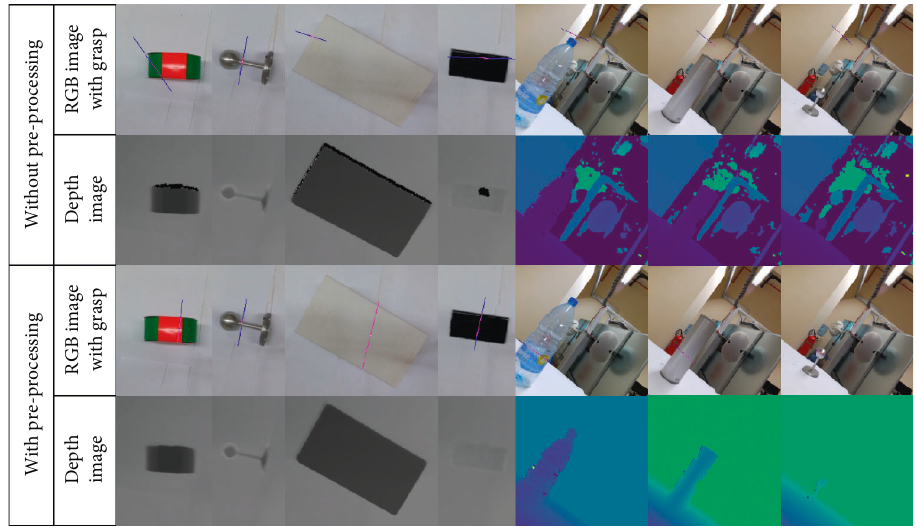
\includegraphics[width=1\textwidth]{img12.png}
	\captionsetup{width=1\linewidth}
	\caption{Grasp generation results: comparison between grasp generated by the GG-CNN
		with and without RGB-D image preprocessing for shiny and black objects
		\cite{sayour2022unknowngrasping}}
	\label{fig:img12}
\end{figure}

One of the main limitations of the approach in \cite{sayour2022unknowngrasping} is the fact
that the grasping pipeline is implemented in MATLAB, therefore hardly portable and hardly
replicable on other robotic hardware. Furthermore grasping with a parallel gripper is
very limited, and the approach can work well with a limited set of objects. The authors
demonstrated a good grasping capability with many different and unknown objects, but
the approach cannot be generalized well without creating a multi-view perspective of
the target object, in order to gain more understanding of the object's shape and
geometry. Although the approach is very promising, there is room for improvement,
especially in the CNN for grasping pose detection, which is the core of the grasping pipeline.


\TODO{add more papers about grasping?}


\section{Autonomous Exploration [todo?]}


\chapter{Robotic Platform for Mobile Manipulation}

This chapter will describe the robotic platform used for the project, specifically the hardware components.
The platform is composed of a mobile robot base, a robotic arm manipulator, sensors and perception systems, 
a soft gripper actuator, 3D-printed mounts, batteries, power management systems, and other electronic devices.
The chapter will also discuss the issues faced during the development of the mobile manipulation platform.

\section{Mobile Robot Platform}

The mobile robot used for the Thesis project is an \textit{AgileX Scout 2.0} robot, depicted in \ref{fig:c3_img01}.
This robot is a skid-steering robot, suitable for outdoor and indoor environments. 
Designed for robotics research and development, the Scout 2.0 is an unmanned ground vehicle (UGV). 
This autonomous mobile robot is CE-certified and offers a robust mechanical design along with capable mobility performance. 
Built to endure diverse conditions, Scout 2.0 features rugged materials and protective casings, ensuring longevity
and reliability during missions. SCOUT 2.0 offers aluminum T-slot rails for secure mounting of external sensors or kits. 
On these rails, a variety of sensors, computers, or other devices are mounted, allowing the creation of a mobile robotic platform
for a wide range of applications, and without relying on power cables to the wall, thanks to its 
\textbf{onboard battery system}.

It supports CAN bus protocol for connections and provides open-source SDK and software resources for expanded capabilities.
Its maximum speed is $1.5 m/s$, and it can carry a payload of $50$ kg. 
The robot is powered by a $24V$ battery, which provides a range of $15$ km maximum. 
The robot is controlled by a ROS-based software system, which allows the control of the robot's speed using a ROS topic
and receiving odometry data from the robot's encoders.

%Add the image of the robot
\begin{figure}[t]
	\centering
	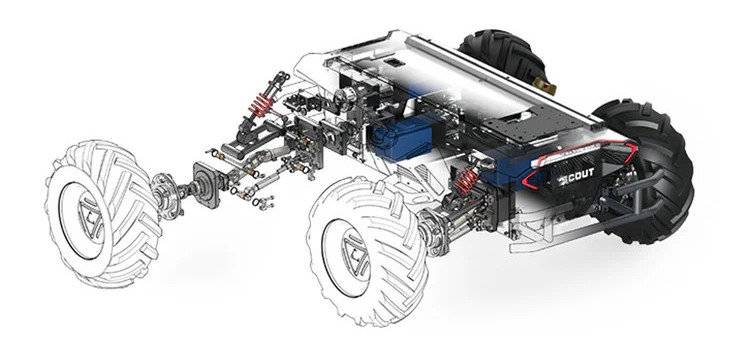
\includegraphics[width=1\textwidth]{chapter3_01.jpg}
	\captionsetup{width=1\linewidth}
	\caption{SCOUT employs 200W brushless servo motors to drive each wheel independently. 
    Its double-wishbone suspension with shock absorbers ensures stability on rough terrain, 
    enabling it to tackle obstacles up to 10cm tall effortlessly.}.
	\label{fig:c3_img01}
\end{figure}

On the mobile robot, an \textit{Intel NUC 12} computer \ref{fig:c3_img02} is mounted.
This \textbf{computer} is used for running all the control
software and the perception algorithms. The computer is connected to a switch, which is used to connect
the computer to the robot's control system and all the sensors and electronic devices mounted on the robot.
The computer is also connected to a router, which is used to connect the computer to the laboratory's network
and the internet. This allows the robot to be controlled remotely via a remote desktop connection.
This computer has the following technical specifications:

\begin{itemize}
    \item Intel Core i7-12700H CPU
    \item 32GB DDR4 RAM
    \item 1TB NVMe SSD
    \item Intel Iris Xe Graphics
    \item Kubuntu 22.04 operating system
\end{itemize}

% Add the image of the computer
\begin{figure}[t]
    \centering
    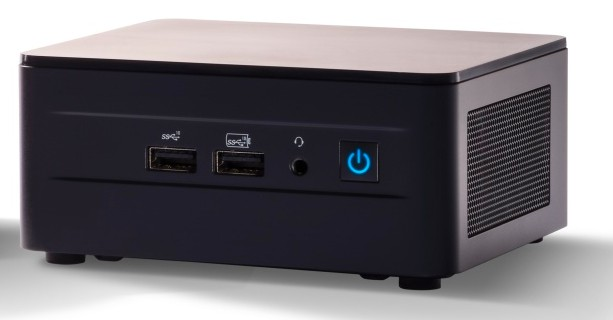
\includegraphics[width=0.6\textwidth]{chapter3_02.jpg}
    \captionsetup{width=1\linewidth}
    \caption{Intel NUC 12 computer mounted on the robot}.
    \label{fig:c3_img02}
\end{figure}

The robot is equipped with an \textit{TP-Link Archer MR200} router and a \textit{Netgear GS108} switch.
The router is used to connect the robot to the laboratory's network and the internet. The router was necessary to
establish a \textbf{remote connection} from a personal laptop to the robot's computer, allowing the control and monitoring
of the robot from a remote location. This was essential for the development of the project, as it allowed me to
work safely with the robot, ensuring that everything was working smoothly and stopping the system in case of any
unexpected behavior or software crashes and malfunctions.

The switch is used to connect the robot's computer to the robot's control system and all the sensors
and electronic devices mounted on the robot. The switch is connected to the router, allowing the robot's computer
to communicate with the laboratory's network and the internet. The robotic arm manipulator is also connected to the switch,
allowing the robot's computer to control the manipulator and receive data from its motors' encoders. 
The LiDAR is connected to the switch, allowing the robot's computer to receive pointcloud data from the LiDAR sensor,
at a fast transmission rate.
 
\section{Robotic Arm Manipulator}

The robotic arm manipulator used for the project is a \textit{Igus ReBeL 6-DoF} \textbf{cobot}, depicted in \ref{fig:c3_img04}.
Cobot is a term used to describe a collaborative robot, which is a robot designed to work alongside humans in a shared workspace.
This cobot is a lightweight, compact, and affordable robotic arm, suitable for research and development
in robotics. It is produced by the German company Igus, which specializes in the production of robotic components
for low-cost automation. The robotic arm is composed of six joints, each driven by a DC motor with an integrated encoder.
The outer contour and mechanical components of the ReBeL utilize Igus® plastic polymers, making it particularly inexpensive
and the lightest cobot on the market. Its lightweight and compact design makes it suitable for mounting on top
of mobile robot platforms, such as the Scout robot. The maximum payload of the arm is $2$ kg, which is more than enough
for the project's requirements. The weight is $8.2$ kg, which is light enough to be carried around by the mobile robot base,
without affecting the robot's mobility and stability.

The \textbf{advantages} of the ReBeL cobot are:

\begin{itemize}
    \item Lightweight, sleek and compact design
    \item Plastic arm, inexpensive and cost-effective
    \item Easy to install and operate with the provided software \ref{fig:c3_img05}
    \item Plug and play proprietary control system, or open-source control option
\end{itemize}

The \textbf{disadvantages} of the ReBeL cobot are:
\begin{itemize}
    \item Limited reach and workspace due to the joints' design and physical constraints
    \item Limited precision and repeatability
    \item The plastic gear components are not as durable and reliable as metal components
\end{itemize}

% Add the of the robotic arm
\begin{figure}[t]
    \centering
    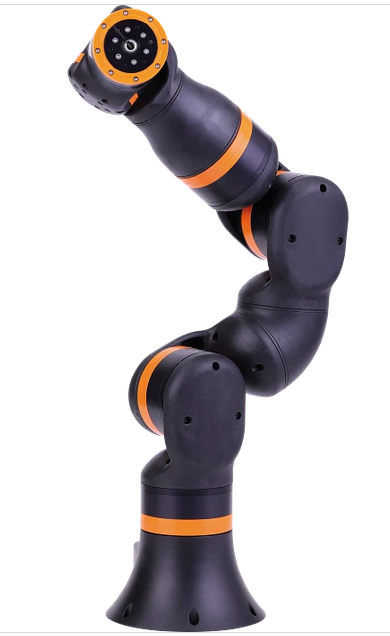
\includegraphics[width=0.3\textwidth]{chapter3_04.png}
    \captionsetup{width=1\linewidth}
    \caption{Igus ReBeL 6-DoF robotic arm (cobot)}.
    \label{fig:c3_img04}
\end{figure}

This robotic arm was the ideal choice for the project since the open-source control option allowed me to develop
the control software for the arm, based on ROS2 software packages. The lightweight and compact design made it suitable
for mounting on top of the SCOUT 2.0 robot, without affecting the robot's mobility and performance. 
The arm's easy installation and operation allowed me to quickly set up the arm and start developing the control software
and perception algorithms for the project.

% Add the image of the robotic arm software
\begin{figure}[t]
    \centering
    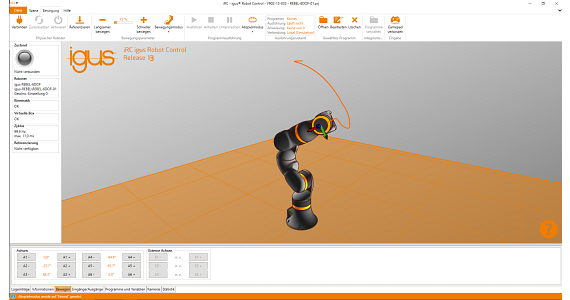
\includegraphics[width=0.8\textwidth]{chapter3_05.png}
    \captionsetup{width=1\linewidth}
    \caption{Igus ReBeL proprietary control software interface}.
    \label{fig:c3_img05}
\end{figure}

\subsection*{Issues with Igus Rebel motors' encoders and calibration}

Throughout the development of the project, I encountered several issues with the Igus ReBeL cobot.
The issues arose when the arm's motors' encoders were not providing accurate position data to the control software.
This caused the arm not to move to the defined joint positions with an accuracy of the end effector of $\pm 0.1mm$,
as specified by the manufacturer in the technical documentation.
This was mainly due to both the calibration of the motors' encoders and the plastic gear components' backlash and play.
The backlash and play in the gear components caused the arm's joints to have a certain amount of free movement before the motor
started to move the joint. This free movement caused the arm's joints to be in an incorrect position, which was not detected
by the motor's encoders. This resulted in the arm jiggling and vibrating when moving to a new joint position, and not reaching
the desired position with a smooth velocity profile.

Furthermore, the main issue encountered was the \textbf{calibration of the motors' encoders}.
This problem slowed down the development
of the project since the software solutions for the calibration of the encoders and the digital zeroing of the joints were not
successful in providing a working solution for the arm's accurate positioning. The calibration of the encoders was necessary
to provide accurate position data to the control software, allowing the arm to move to the desired joint positions with high
precision. The problem encountered was that the software for the automatic calibration of the motor controllers did not work
as expected, resulting in errors and faulty calibration of the encoders. The only solution was to replace the entire robot
arm with a new one, correctly calibrated by the manufacturer.

\section{Sensors and Perception}

The mobile robot platform is equipped with several sensors and perception systems, which are essential for the project's
objectives. The sensors and perception systems are used for mapping and localization, obstacle avoidance, object detection
and recognition, and manipulation tasks. 
Two main sensors are installed on the robot: a 3D LiDAR sensor and an RGB-D stereo camera sensor.
The LiDAR sensor is in a fixed position, on top of the robot to have a 360-degree field of view, while the camera sensor
is mounted on the robotic arm's wrist, allowing the camera to move with the arm's end effector.

\subsection{3D LiDAR Sensor}

The main sensor for environment perception for localization and navigation is mounted on the robot's T-slot rails.
The sensor is a \textit{Ouster OS1-64} LiDAR sensor, as shown in \ref{fig:c3_img06}.
The OS1 offers clean, dense data across its entire field of view for accurate perception and crisp detail in industrial,
automotive, robotics, and mapping applications.
This sensor is a \textbf{64-plane LiDAR sensor}, capable of providing a 360-degree field of view with a range of $120$ meters. 
The sensor has a resolution of $\pm 0.1cm$ and a stable scan rate of $10 Hz$ at $1024$ points resolution.
The vertical and horizontal scan resolution are $\pm 0.01$°.
Its minimum range of $0.5$ meters makes it suitable for indoor environments, while its maximum range of $120$ meters
makes it suitable also for outdoor environments.
This sensor was employed to create maps of the environments and also to localize the robot within the environment.
It proved also useful for dynamic obstacle avoidance, thanks to its high resolution and scan rate.

%insert image of the LiDAR sensor
\begin{figure}[t]
    \centering
    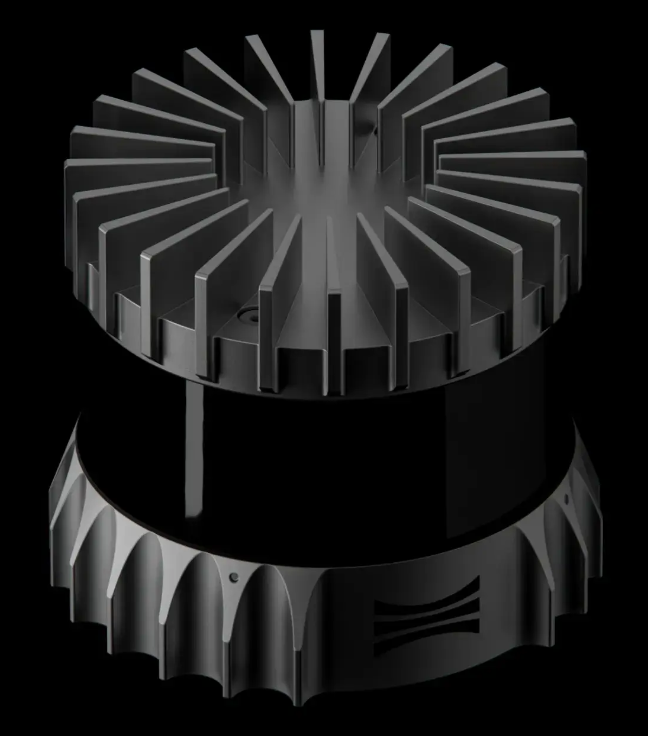
\includegraphics[width=0.5\textwidth]{chapter3_06.png}
    \captionsetup{width=1\linewidth}
    \caption{Ouster OS1-64 LiDAR sensor}.
    \label{fig:c3_img06}
\end{figure}

\subsection{RGB-D Stereo Camera Sensor}

The robotic arm is equipped with a \textit{Intel Realsense D435} RGB-D stereo camera sensor, shown in \ref{fig:c3_img07}.
This camera is mounted on the \textit{wrist} of the robotic arm, allowing the camera to move with the arm's end effector.
The camera is used for object detection and recognition, and also for Aruco markers detection and pose estimation.
This is the camera of choice for robotic applications, as it provides both RGB and depth images, which are essential
for perception tasks in robotics. The camera is also lightweight and compact, making it suitable for mounting on the cobot.

The Intel RealSense D435 is a stereo depth camera that is designed for capturing RGB and depth images.
The camera is equipped with a global shutter and a rolling shutter, which allows it to capture images with a resolution
of $1920\times1080$ pixels at $30$ frames per second, even though the ROS2 driver provided by Intel reduces the resolution
to $640\times480$ pixels at $30$ frames per second. The camera has a field of view of $85.2$° horizontal, $58$° vertical,
and $94$° diagonal. The depth camera works within a range of $0.3$ meters to $3$ meters while maintaining 
high accuracy and precision.

% Add an image of the camera
\begin{figure}[t]
    \centering
    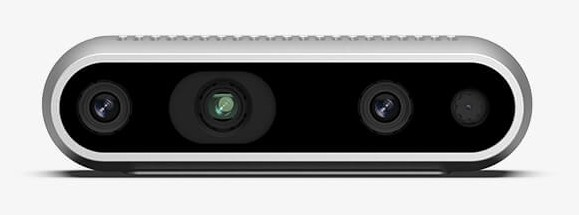
\includegraphics[width=0.5\textwidth]{chapter3_07.jpg}
    \captionsetup{width=1\linewidth}
    \caption{Intel RealSense D435 RGB-D stereo camera}.
    \label{fig:c3_img07}
\end{figure}

\subsection{Issues with Intel Realsense calibration}

The camera provided by the laboratory was not calibrated correctly, especially the depth estimations were not accurate.
In fact, the depth images provided depth estimations that were not consistent with the real-world distances of the objects
in the environment. I was able to discover such issues when I started using the camera's depth sensor for the perception
tasks of the project. I realized that the estimated distance from the camera and the Aruco markers (the distance estimated
using geometrical calculations and the camera's intrinsic parameters) was \textbf{not consistent} with the estimated distance
to the marker provided by the camera's depth sensor. This inconsistency was due to the camera's depth sensor not being
calibrated correctly.

% Add the image of the calibration pattern
\begin{figure}[t]
    \centering
    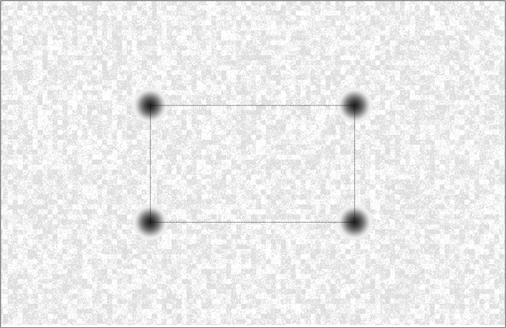
\includegraphics[width=0.5\textwidth]{chapter3_08.png}
    \captionsetup{width=1\linewidth}
    \caption{Calibration pattern used for the camera's depth image calibration}.
    \label{fig:c3_img08}
\end{figure}

This issue was critical for the project, as the depth sensor was used for many perception algorithms.
I managed to solve this issue by calibrating the camera's depth sensor using the proprietary software provided by Intel:
\textit{Interl Realsense Self-Calibration Tool}, an application for \textbf{automatic on-chip calibration}.
The calibration process was straightforward and required a few minutes to complete, even though many trials were needed
to find the best possible calibration parameters. Two calibration procedures were carried out:

\begin{itemize}
    \item \textbf{Intrinsic parameters calibration}: this calibration process was used to calibrate the camera's 
    intrinsic parameters,
    such as the focal length, principal point, and distortion coefficients. This calibration was necessary to correct
    the distortion of the images and to provide accurate depth estimations from the RGB sensor. The calibration process
    required the camera to capture a series of images of a calibration pattern (checkerboard pattern) from different angles
    and distances. The calibration software then used these images to estimate the intrinsic parameters of the camera.
    \item \textbf{Depth sensor calibration}: this calibration process required the camera to capture a series of
    depth images of a calibration sheet \ref{fig:c3_img08}, which was a flat surface with known distances between the points.
    The calibration software then used these depth images to estimate the depth sensor's parameters, 
    such as the depth scale factor and the depth offset. 
    These parameters were necessary to correct the depth estimations of the camera's depth sensor.
\end{itemize}


After the calibration process, the camera's depth sensor was providing accurate and consistent depth estimations,
which were consistent with the real-world distances of the objects in the environment.

\section{Soft Gripper Actuator}

The robotic arm is equipped with a Soft Gripper Pneumatic Actuator from \textit{Soft Gripping}, depicted in \ref{fig:c3_img09}.
This gripper is composed of 3 soft fingers, which are actuated by a pneumatic pump. The fingers are made of
\textbf{silicone rubber}, which is soft and flexible, allowing the gripper to grasp and manipulate objects of different shapes
and sizes. The silicone material of the fingers is also non-slip, which ensures a secure grip on the objects.
It is also essential in food industries, where the gripper is used to handle delicate and fragile objects, 
such as fruits. The other advantage is that silicone is non-toxic and food-safe, making it suitable for handling
food products.

% Add the image of the soft gripper
\begin{figure}[t]
    \centering
    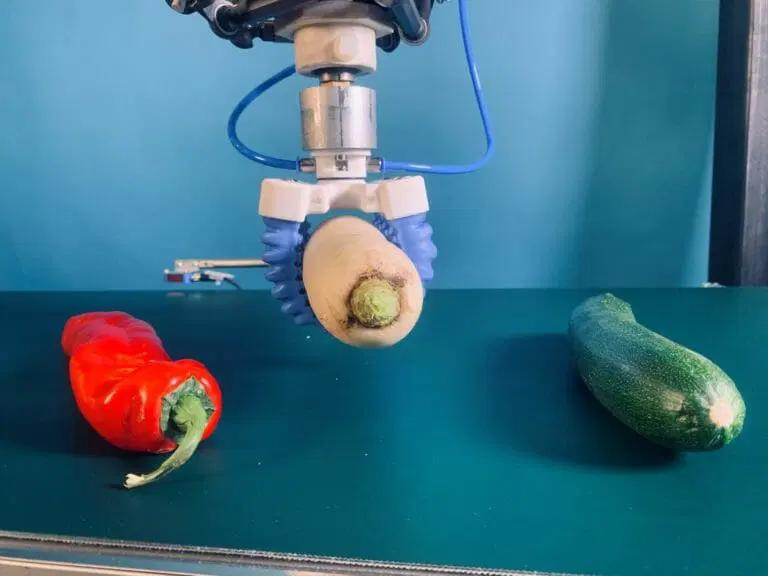
\includegraphics[width=0.6\textwidth]{chapter3_09.jpg}
    \captionsetup{width=1\linewidth}
    \caption{Soft Gripper Pneumatic Actuator handling vegetables}.
    \label{fig:c3_img09}
\end{figure}

The soft gripper is controlled by a pneumatic pump \ref{fig:c3_img13}, which provides compressed air to the fingers,
allowing them to open and close. The pneumatic system works at a pressure of $1$ bar when the fingers are closed, and at
a negative pressure of $0$ bar when the fingers are opened. The pneumatic pump that controls the soft gripper
allows the user to set the pressure value used when closing the fingers, but the pressure value cannot be
changed dynamically via electronic control. Figure \ref{fig:sg_combined} shows the soft gripper mounted on the end effector
with the fingers opened and closed.

% Add a picture of the pneumatic pump
\begin{figure}[t]
    \centering
    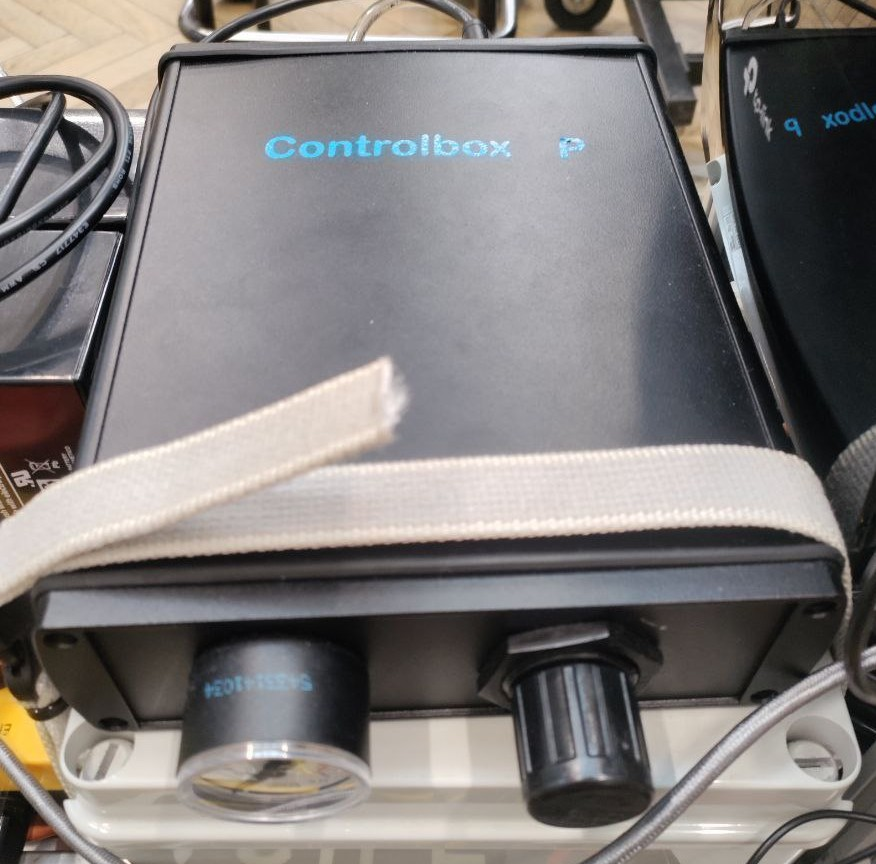
\includegraphics[width=0.6\textwidth]{c3_13.jpg}
    \captionsetup{width=1\linewidth}
    \caption{Pneumatic Pump control box secured on top of the mobile robot}.
    \label{fig:c3_img13}
\end{figure}

The pneumatic pump provided with the soft gripper has only one output tube used for providing positive pressure
to the fingers. The negative pressure is provided by the environment, as the fingers are opened by the air pressure
inside the fingers, which is lower than the air pressure outside the fingers. 
Other versions of the pneumatic pump provide also a negative pressure output tube, which allows the user to control
the pressure value used when opening the fingers, but this feature requires an external vacuum compressor to work.

The gripper is mounted on the robotic arm's end effector, allowing the arm to grasp and manipulate
objects in the environment. It is placed strategically close to the robotic arm's flange to ensure
that the mobility and reach of the end effector are not affected by the gripper's size.
Furthermore, the soft gripper is very lightweight and compact, making it suitable for mounting on the cobot.

% Add pictures of the gripper opened and closed
\begin{figure}[t]
    \centering
    \begin{subfigure}{0.45\textwidth}
        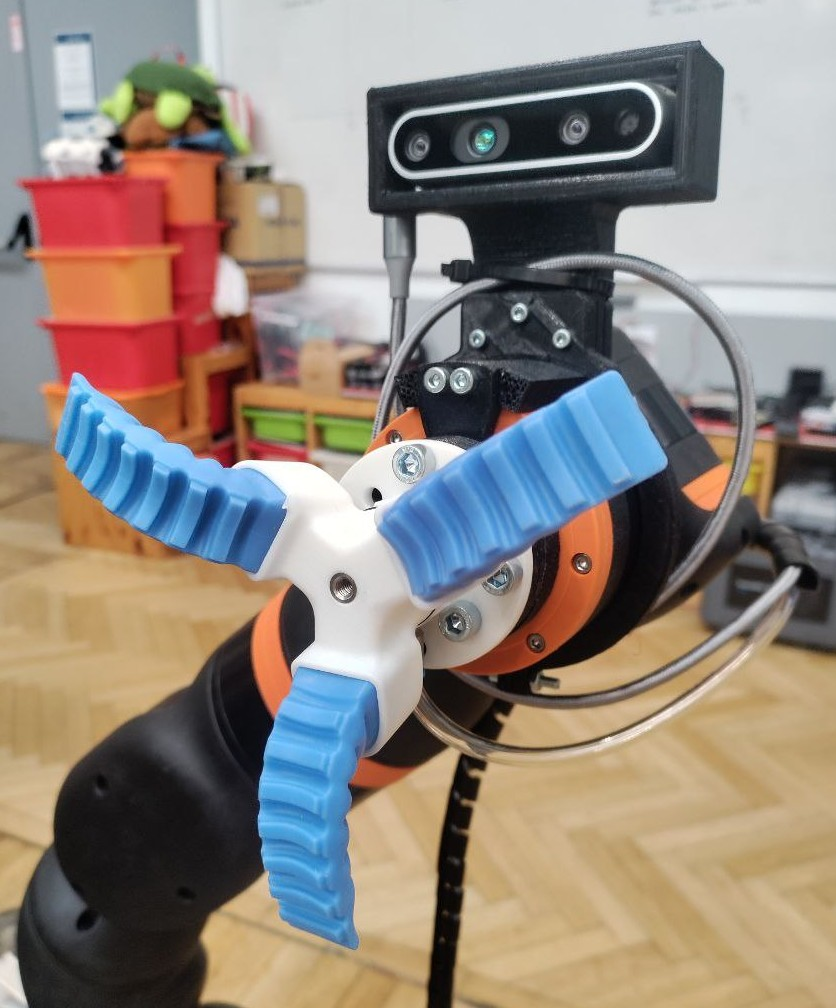
\includegraphics[width=1\textwidth]{c3_26.jpg}
        \caption{Soft Gripper opened}
        \label{fig:opened}
    \end{subfigure}
    \hfill % Optional: Adds space between images
    \begin{subfigure}{0.45\textwidth}
        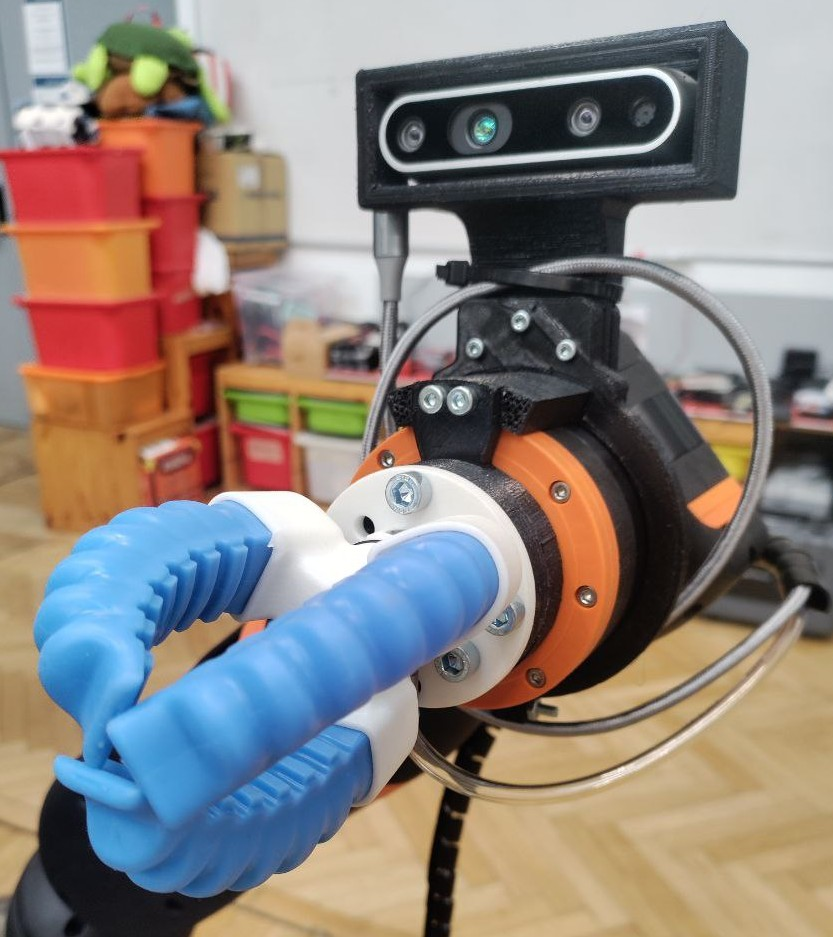
\includegraphics[width=1.07\textwidth]{c3_25.jpg}
        \caption{Soft Gripper closed}
        \label{fig:closed}
    \end{subfigure}
    \caption{Soft Gripper mounted on the end effector}
    \label{fig:sg_combined}
\end{figure}

The pneumatic pump is provided without any power supply, so it was necessary to create a system to power the pump
using the \textbf{onboard batteries}. The pump is powered by a 24V lead battery, which is the same battery powering
the robotic arm. I created a system for powering both the robotic arm and the pneumatic pump with the same battery,
using Molex cables and connectors. These Molex cables proved to be a reliable and optimal solution,
as they allowed me to switch easily between the onboard batteries and the external cobot power supply.
The Molex cable management is shown in \ref{fig:c3_img12}.
In fact, the cobot's power supply provides 24V at a maximum of 10A, which is enough to power the robotic arm
and the pneumatic pump simultaneously, since the pneumatic pump doesn't require a high current to operate.
The cable of the external power supply is also a Molex cable, so that's why I used Molex connectors and cables
to connect the robotic arm and the pneumatic pump to the cobot's power supply.

% Add a picture of the Molex connectors and cables
\begin{figure}[t]
    \centering
    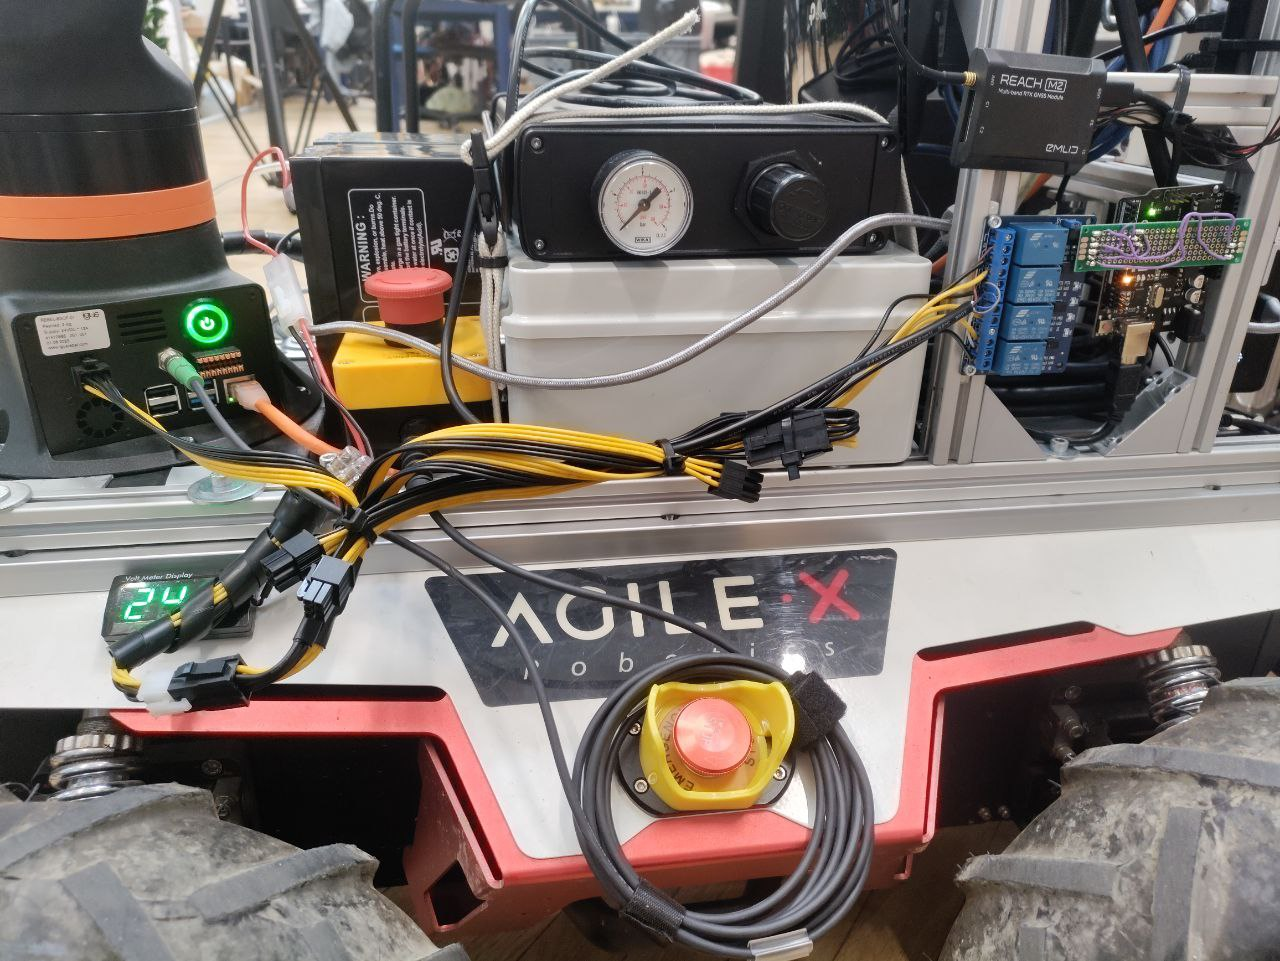
\includegraphics[width=0.6\textwidth]{c3_12.jpg}
    \captionsetup{width=1\linewidth}
    \caption{Molex connectors and power management for the cobot, pump, and relays}.
    \label{fig:c3_img12}
\end{figure}

The pneumatic pump must be controlled at 24V, as the pump's solenoid valve requires this voltage to operate.
The pump provides 4 digital pins for controlling its operation, which are used to open and close the fingers.
I created a simple system capable of controlling the pump's operation using an \textbf{Arduino UNO microcontroller}.
The Arduino UNO is connected to the robot's computer via USB, allowing the computer to send commands to the Arduino
via the serial port. The Arduino UNO is then connected to the pneumatic pump via a relay module,
composed of 4 different relays, each controlling a different digital pin of the pump. The relays were necessary
to provide an output voltage of 24V, while the Arduino UNO provides only 5V via its digital pinout.
The relays are cheap and quick enough to switch between the digital pins of the pump, allowing efficient
control of the pump's operation, and the installation of simple circuitry for the control system 
directly on the mobile robot platform. Figure \ref{fig:c3_img10} shows the Arduino UNO microcontroller
and the relay module used to control the pneumatic pump.

% Add a picture of the Arduino UNO and the relay module
\begin{figure}[t]
    \centering
    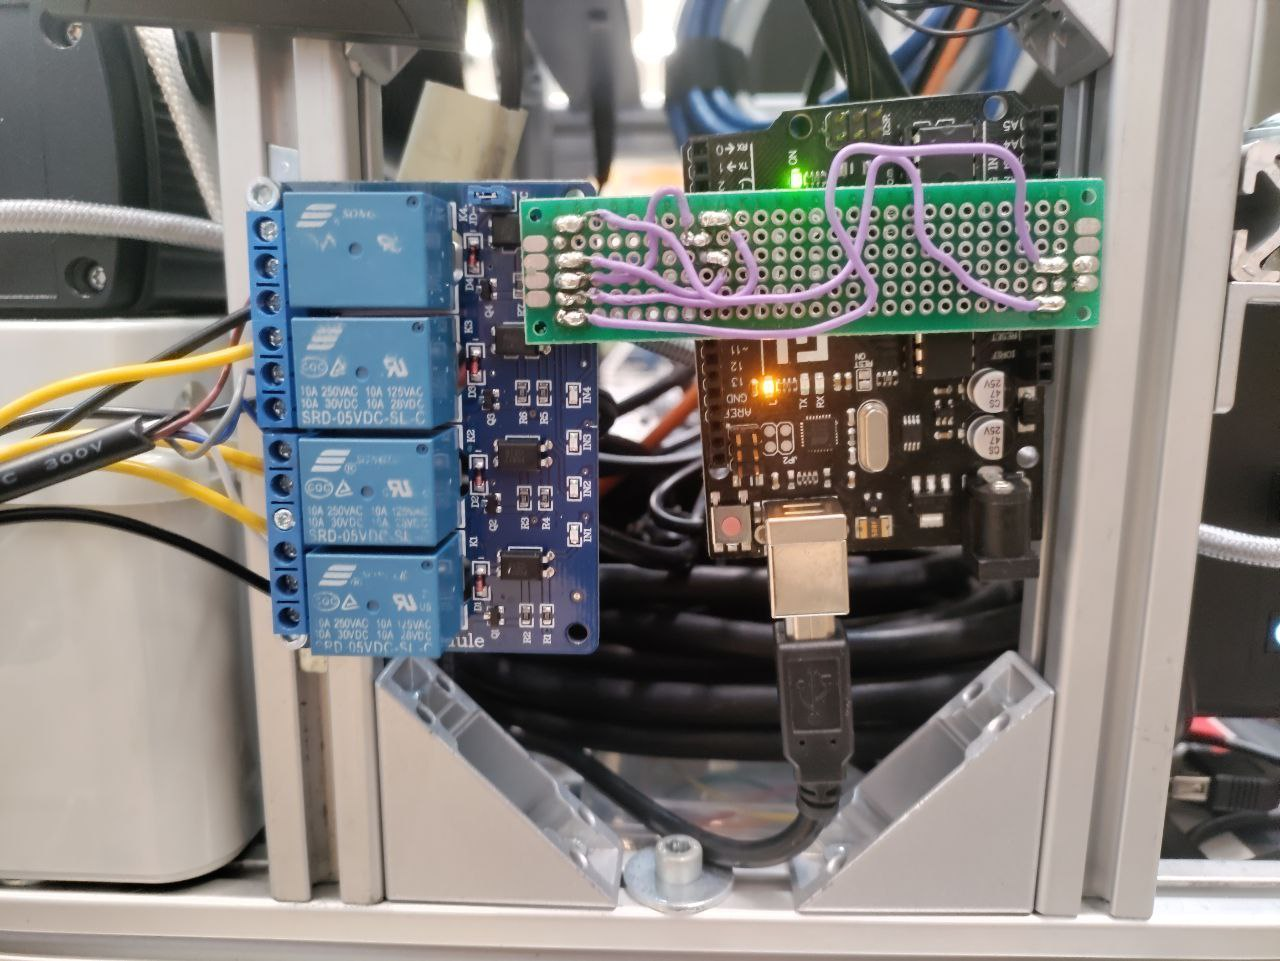
\includegraphics[width=0.6\textwidth]{c3_11.jpg}
    \captionsetup{width=1\linewidth}
    \caption{Arduino UNO microcontroller and relay module used to control the pneumatic pump}.
    \label{fig:c3_img10}
\end{figure}

\section{3D Printed Mounts Design}

Mounting the sensors and electronic devices on the mobile robot platform required the design and 3D printing
of custom mounts. The mounts were designed using the \textit{Fusion 360} CAD software, which allowed me to create
precise and accurate models of the mounts. The mounts were then 3D printed using the laboratory's 3D printer,
which is a \textit{Creality CR-10S} 3D printer. 

I designed and created the \textbf{mount for the GPS antenna}, which was used for outdoor localization
and navigation tasks. The GPS antenna mount was designed to be placed on top of the LiDAR sensor, ensuring
that the antenna had a clear view of the sky and the satellites. The mount was also designed to be lightweight
and quick to install, without affecting the LiDAR sensor's field of view, and without using any screws or bolts.
Figure \ref{fig:gpsprint} shows the mount installation on top of the LiDAR sensor, while Figure \ref{fig:gps3d}
shows the 3D design of the mount.
I never used the GPS in my project, but the support that I created for it was used by other researchers 
in the laboratory for other projects.

% Add pictures of the GPS antenna mount render and 3D print
\begin{figure}[t]
    \centering
    \begin{subfigure}{0.3\textwidth}
        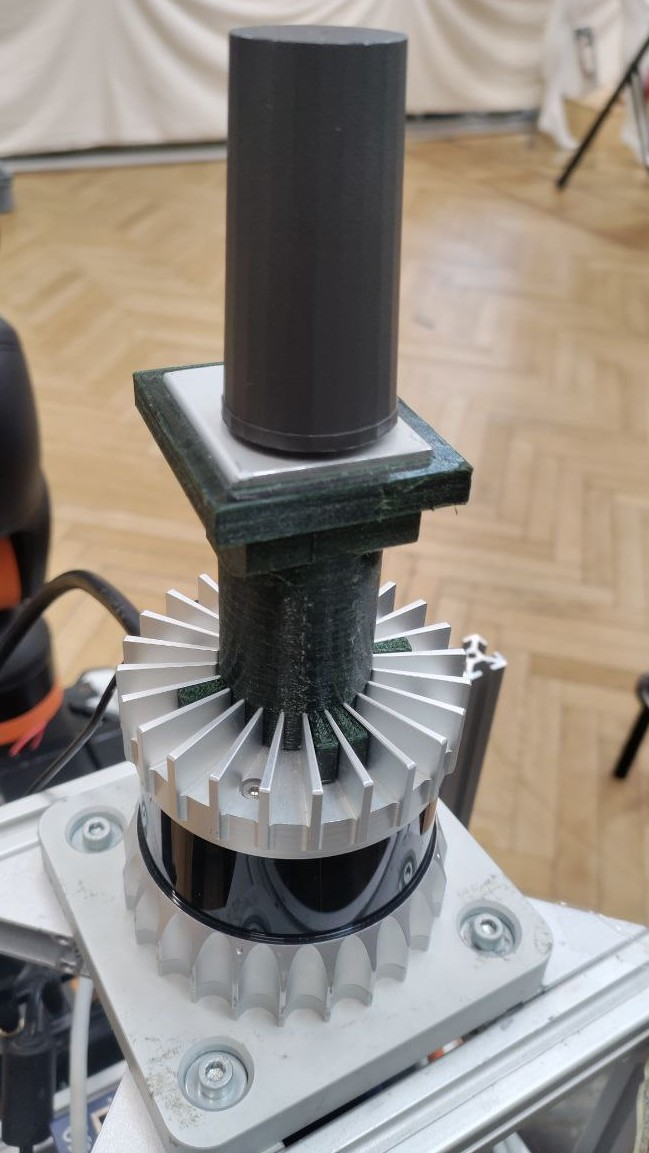
\includegraphics[width=0.7\textwidth]{c3_20.jpg}
        \captionsetup{width=0.9\linewidth}
        \caption{GPS antenna 3D-printed mount}
        \label{fig:gps3d}
    \end{subfigure}
    \hfill
    \begin{subfigure}{0.67\textwidth}
        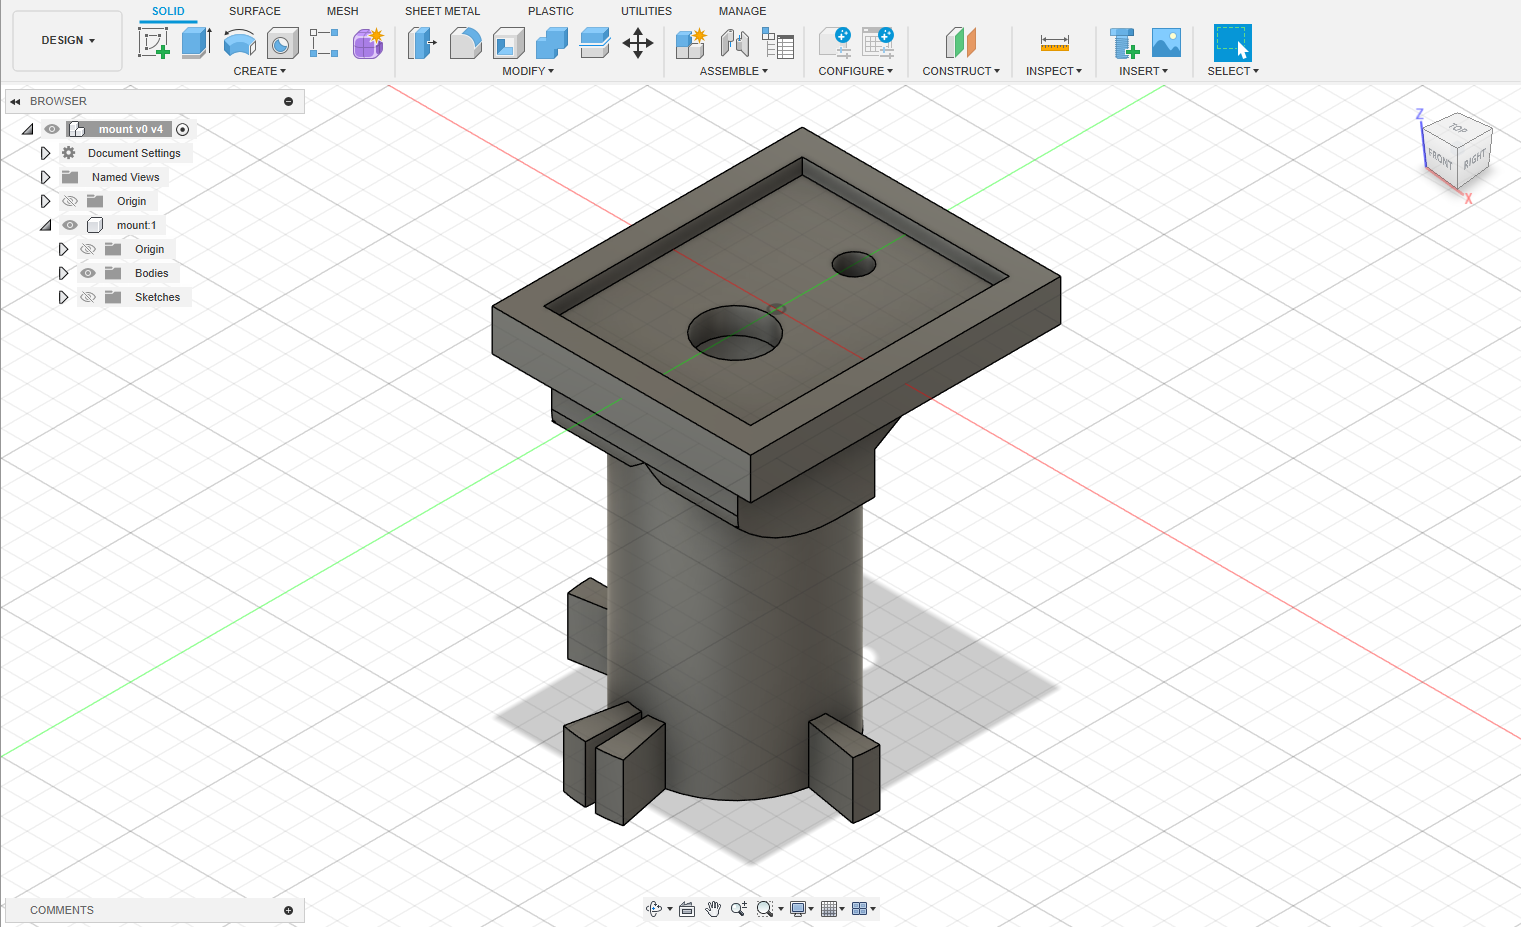
\includegraphics[width=1.0\textwidth]{c3_22.png}
        \caption{3D design}
        \label{fig:gpsprint}
    \end{subfigure}
    \captionsetup{width=1\linewidth}
    \caption{GPS antenna mount design and 3D-print on top of the LiDAR}.
    \label{fig:c3_gps}
\end{figure}

The 3D printer that I used in the AIRLab is a Fused Deposition Modeling (FDM) printer,
which uses a thermoplastic filament to create the 3D models layer by layer. The material of choice
for the 3D prints was \textit{PETG} (Polyethylene Terephthalate Glycol), which is a strong and durable material,
suitable for mechanical parts and mounts. The PETG material is also resistant to mechanical stress and heat,
making it the ideal material for the mounts for these kinds of applications.

I designed and printed two versions of the mount for the cobot's flange:

\begin{itemize}
    \item \textit{Mount V1} \ref{fig:mountv1}: a mount for the Realsense camera and a digital button on top of a cylinder used
    for pressing buttons on a control panel. The mount was designed to be robust and easy to switch with other
    mount extensions. This mount was used for the first demos and tests of the project.
    \item \textit{Mount V2} \ref{fig:mountv2}: a mount for the Realsense camera and the soft gripper as an end-effector.
    This mount was designed to be compact, robust, and more effective for the final versions of the project.
\end{itemize}

The 3D-printed mounts were designed to be lightweight and compact, to ensure that the robot's mobility and stability
were not affected. The mounts were also designed to be very robust and durable, to withstand the vibrations and shocks
of the mobile robot platform. The mounts are not very easy to install and remove, since they are designed to be
mounted with several screws and bolts, ensuring that the sensors and electronic devices are securely attached to the robot.
These mounts demonstrated to be very effective and reliable, as they withstood the vibrations while maintaining
the sensors in their fixed position.

\subsection{Mount V1}

% Add pictures of the Mount V1 render and 3D print
\begin{figure}
    \centering
    \begin{subfigure}{\textwidth}
        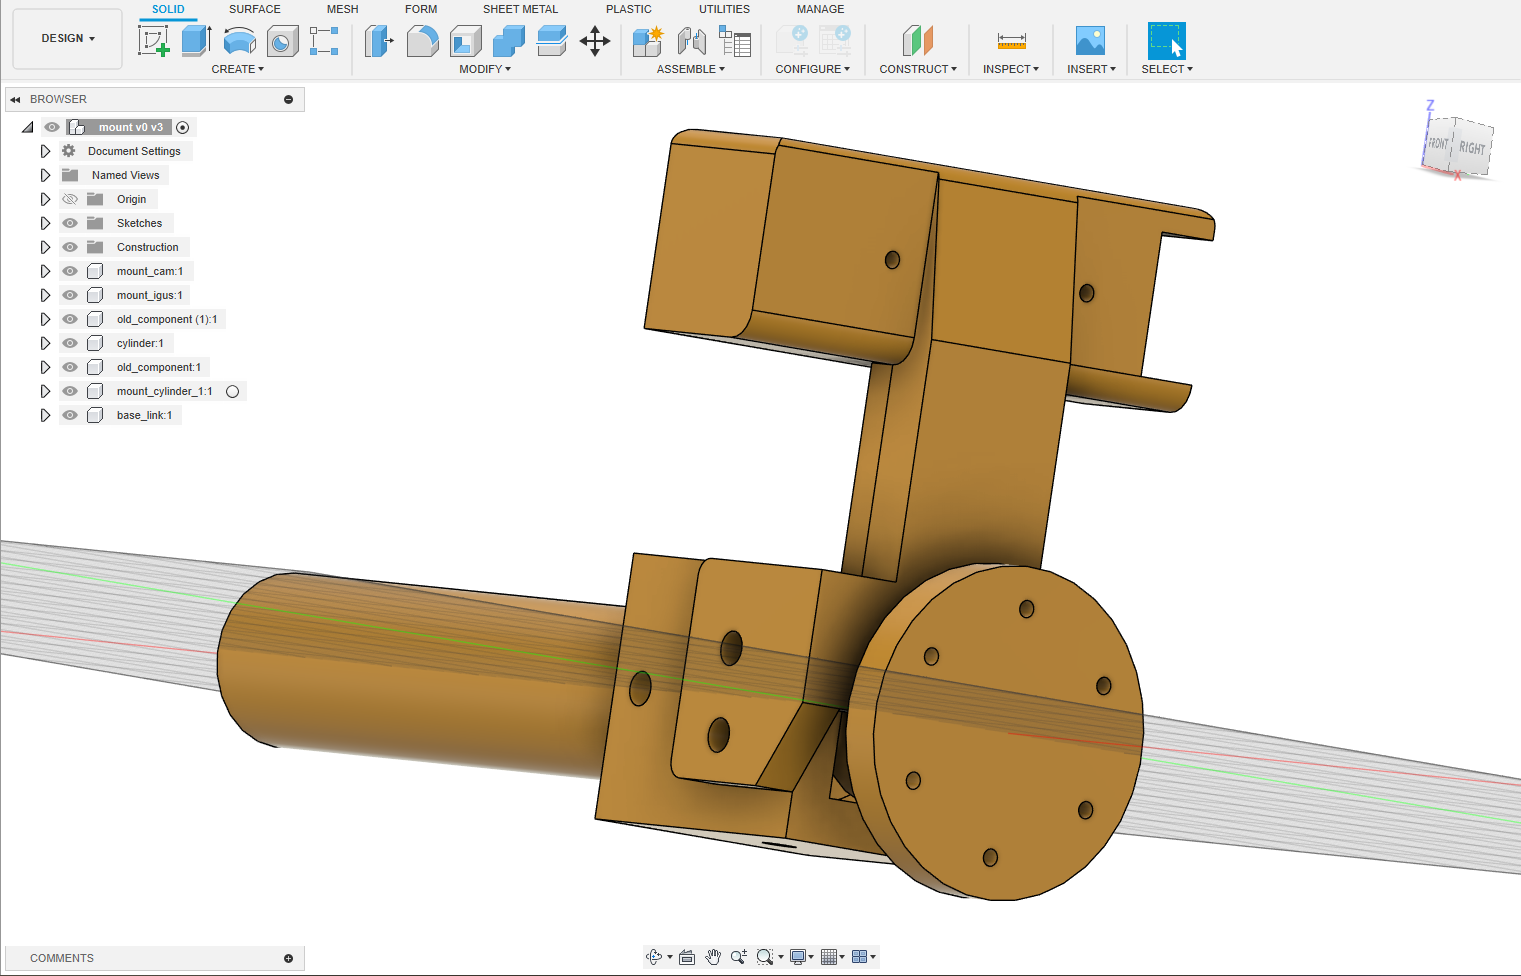
\includegraphics[width=0.9\textwidth]{c3_20.png} % Replace with your image file
        \caption{Back side view of the 3D design}
        \label{fig:frontv1}
    \end{subfigure}
    
    \vspace{1em} % Add some vertical space between images (adjust as needed)

    \begin{subfigure}{\textwidth}
        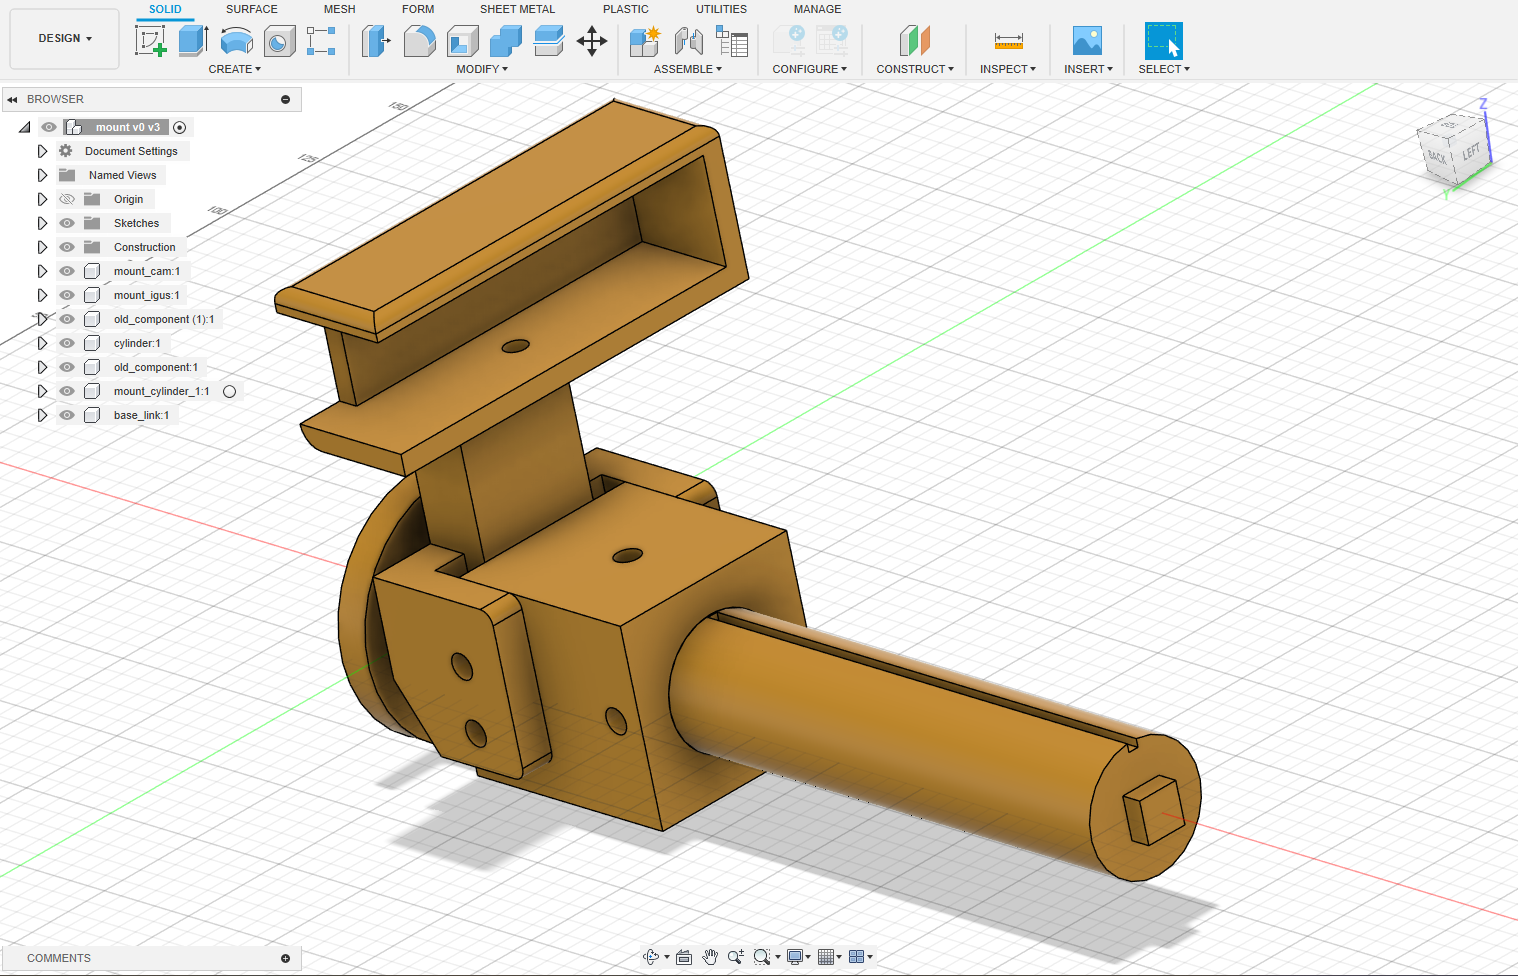
\includegraphics[width=0.9\textwidth]{c3_23.png} % Replace with your image file
        \caption{Frontal side view of the 3D design}
        \label{fig:sidev1}
    \end{subfigure}

    \caption{MountV1 Design screenshots from \textit{Autodesk Fusion 360}}
    \label{fig:mountv1}
\end{figure}

The first version of the mount, alias \textit{Mount V1}, shown in \ref{fig:mountv1},
was designed to be robust and easy to switch with other mount extensions. 
The mount was designed to be lightweight and long, to ensure that the cobot's end effector
would be able to reach objects not in the immediate vicinity of the robot. The mount was also designed to be
compact, with the stereo camera mounted in front of the cobot's flange, and the digital button mounted on top
of a cylinder used for pressing buttons on a control panel. The mount was also designed to be very robust and durable.

After many tests, the cylinder was then shrunk to a smaller length, to ensure that the cobot's end effector
mobility and reach were not affected negatively. This allowed the cobot's end effector to reach objects
in the vicinity with fewer limitations and constraints on its orientation.
The digital button placed on the tip was initially used as a digital feedback mechanism for the pressure
of the buttons on the control panel. This button was later removed, as it was not necessary for the project's
objectives. The mount was then used for the first demos and tests of the project, and it proved to be very effective.

One of the main issues encountered with the mount was the \textbf{reduced field of view of the stereo camera}, due to its
installation on the cobot's flange. The camera was placed at the right distance from the center of the cobot's flange,
making it possible for the camera's field of view not to be obstructed by the cylinder.
After many tests, I realized that the best configuration would be to mount the camera on top of the wrist,
to enlarge the field of view. The Mount V1 was used for the "button presser demo", and replaced with its 
second improved version for the next demos.

\subsection{Mount V2}

% Add pictures of the Mount V2 render and 3D print
\begin{figure}
    \centering

    \begin{subfigure}{\textwidth}
        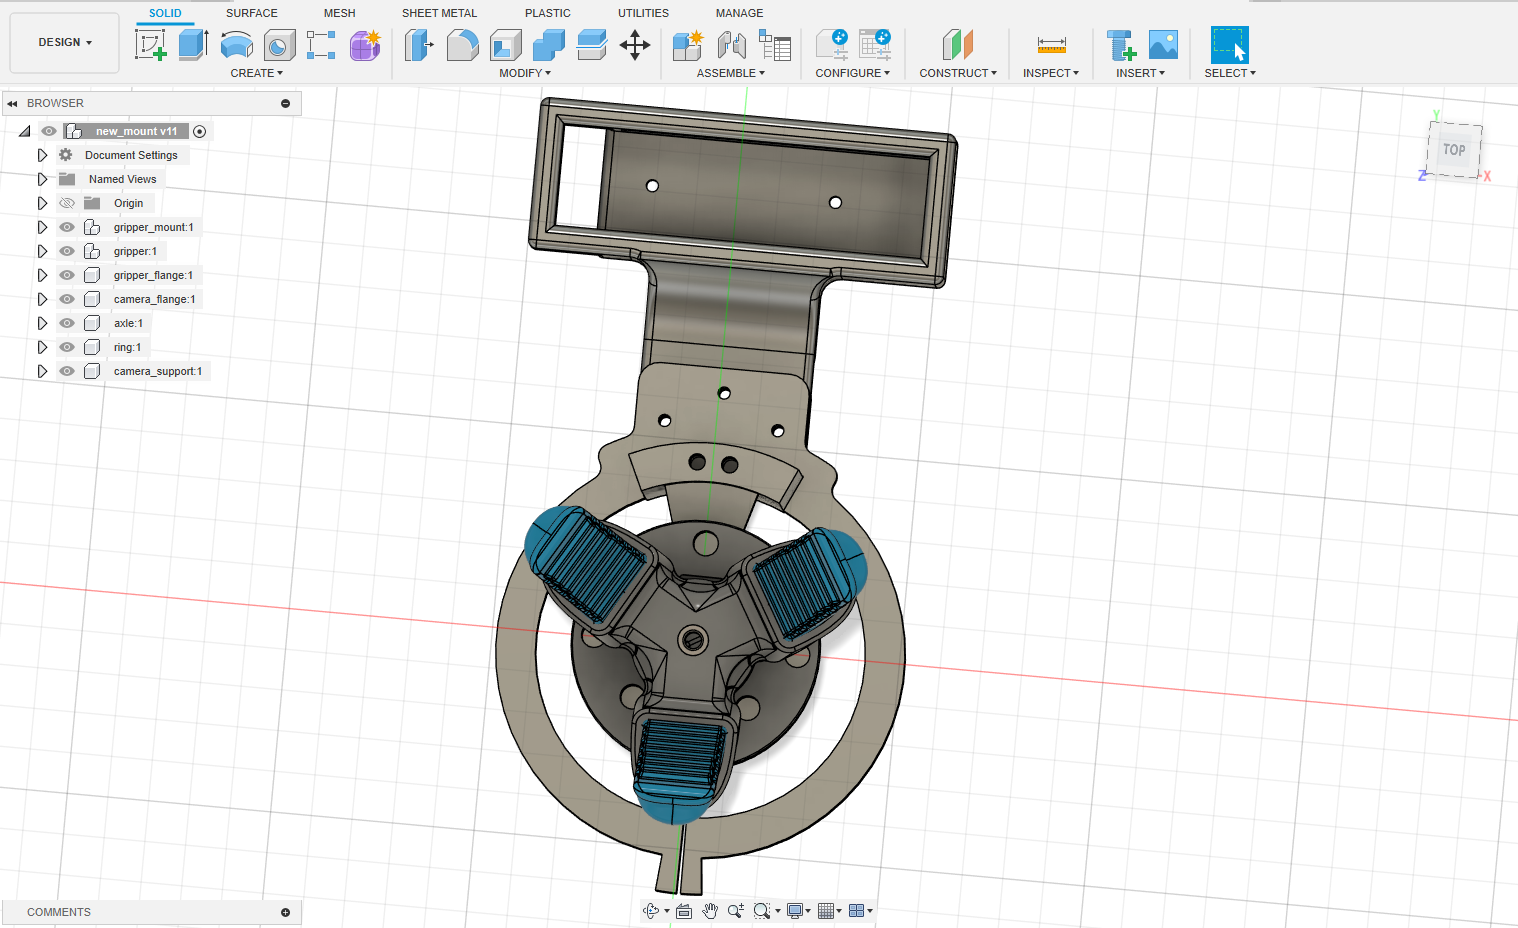
\includegraphics[width=\textwidth]{c3_21.png} % Replace with your image file
        \caption{Front view of the 3D design}
        \label{fig:frontv2}
    \end{subfigure}
    
    \vspace{1em} % Add some vertical space between images (adjust as needed)

    \begin{subfigure}{\textwidth}
        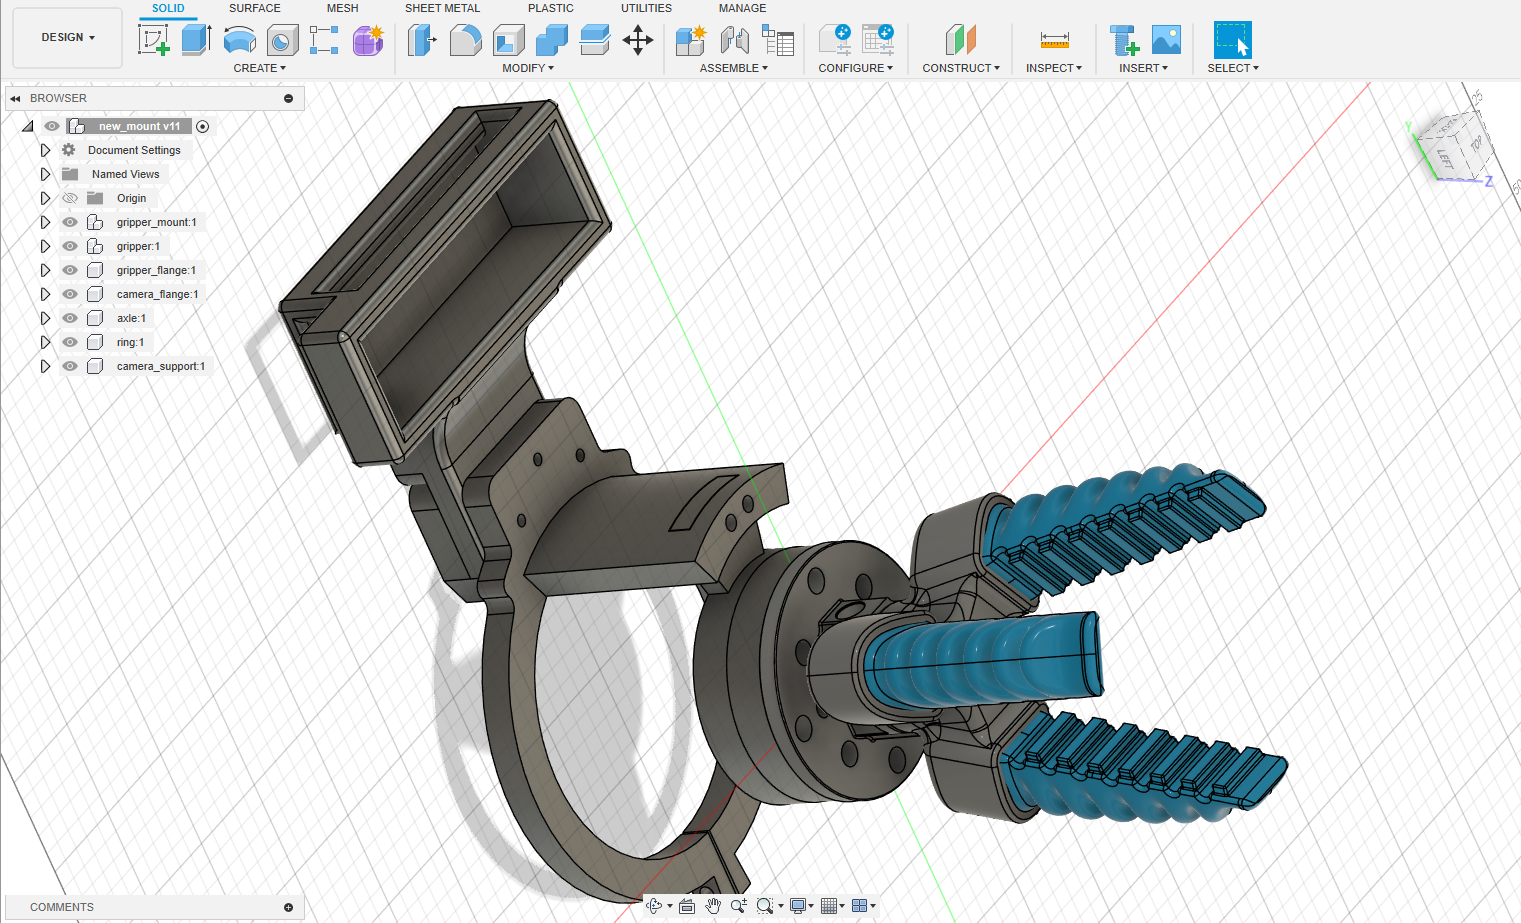
\includegraphics[width=\textwidth]{c3_24.png} % Replace with your image file
        \caption{Side view of the 3D design}
        \label{fig:sidev2}
    \end{subfigure}

    \caption{MountV2 Design screenshots from \textit{Autodesk Fusion 360}}
    \label{fig:mountv2}
\end{figure}

The second version of the mount, alias \textit{Mount V2}, was designed to be compact, robust, and more effective
for the final versions of the project and the "soft grasping" demos. The mount,
shown in \ref{fig:mountv2}, comprises 3 parts:
the flange connector, the camera mount, and the soft gripper mount. The flange connector is used to connect
the mount to the cobot's flange, ensuring that the mount is securely attached to the cobot. The camera mount
is used to mount the stereo camera on top of the cobot's wrist, ensuring that the camera has a wider field of view.
The soft gripper mount is used to mount the soft gripper on the cobot's flange connector, allowing the cobot's
end effector to grasp and manipulate objects in the environment.

The \textbf{flange connector} was designed from scratch because the flange provided by the cobot's manufacturer was not
compatible with the soft gripper mount. The flange connector was designed to be lightweight and compact, 
to ensure that the 3d printing process would be fast and structurally sound. The flange connector was also designed
to be robust and durable, to withstand the vibrations and shocks of the cobot's movements.
The camera mount is designed to be attached to the flange connector on the cobot's wrist with screws and bolts,
ensuring that the camera is securely attached to the cobot while preventing vibrations that could
offset the sensor position and orientation. The camera mount is designed to host the camera cable angled connector.
This angled connector is magnetic, and it prevents the cable from being pulled out of the camera when
the cobot's end effector moves around. This was a critical feature, set to avoid the camera's cable
being broken or damaging the internal USB-C port of the stereo camera. The MountV2 installed on the cobot
is shown in \ref{fig:c3_img17}.

\begin{figure}[t]
    \centering
    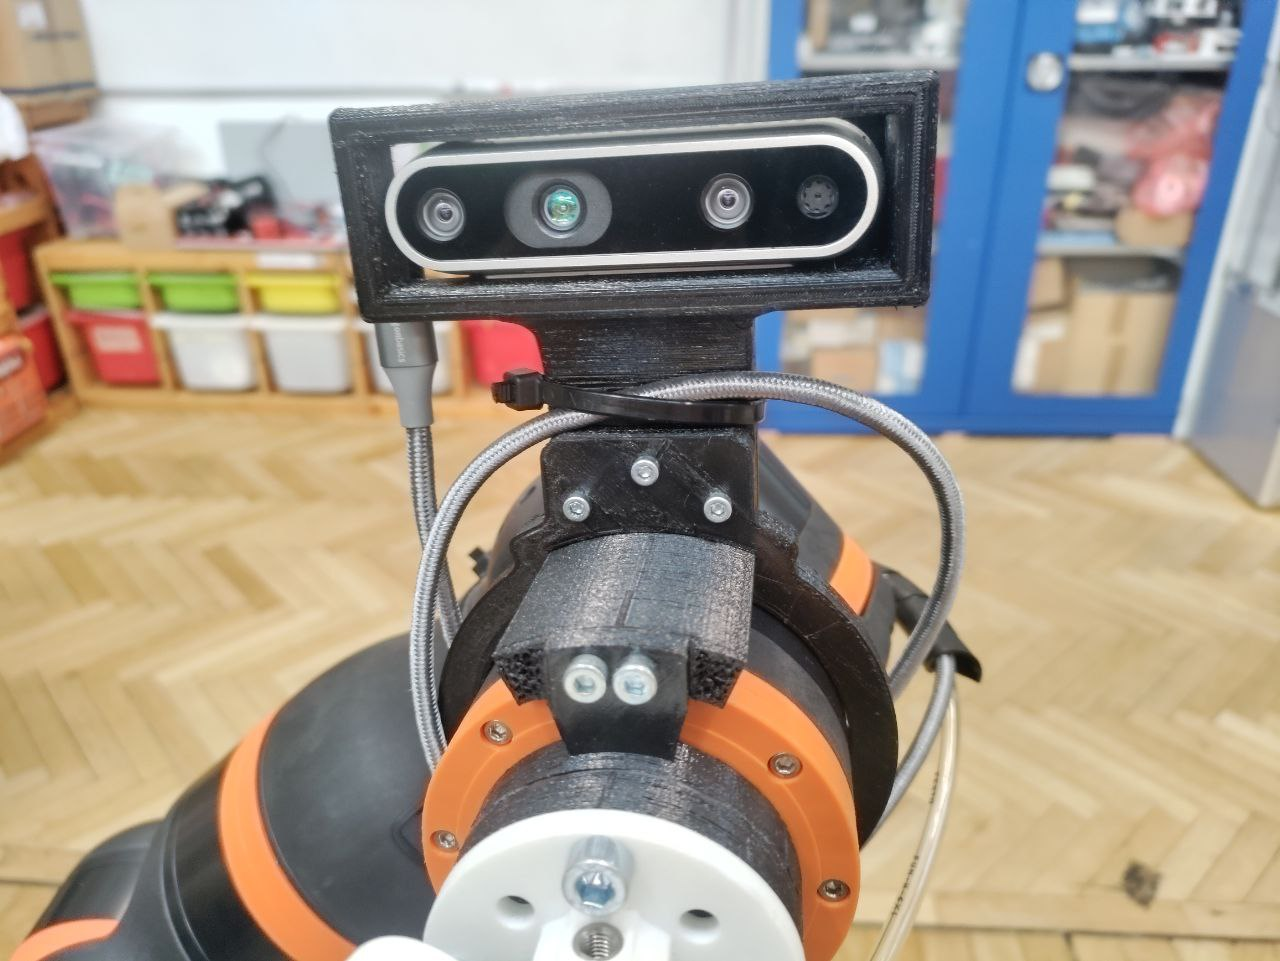
\includegraphics[width=0.6\textwidth]{c3_17.jpg}
    \captionsetup{width=1\linewidth}
    \caption{3d-printed mountV2 on the arm's wrist}.
    \label{fig:c3_img17}
\end{figure}

\subsection{Issues with the laboratory's 3D printer}

The 3D printer in the AIRLab is a printer that is used by many researchers and students for their projects.
In the past, very little maintenance was done on the printer, and the printer was not calibrated correctly.
This caused many issues with the 3D prints, such as \textbf{stringing, and under-extrusion}, which affected negatively 
the quality of my prints. Therefore I had to carry out maintenance on the printer to fix these issues.
I calibrated the printer's bed and the extruder, to ensure that the prints were of high quality and accurate.
I substituted the nozzle with a new one, and unclogged the hotend, to ensure that the filament was extruded correctly
and in the right amount. I also cleaned the printer's bed and the extruder, to ensure that the prints were sticking
correctly to the bed. After these maintenance operations, the printer was working correctly, and the prints were of
higher quality, even though they were still far from being perfect. I was not able to clean the printer's
extruder gears and the filament feeder, as they were not accessible to me due to some screws being stripped.

\section{Batteries and Power Management}

The mobile robot's internal battery is capable of powering all the sensors and computational
units that are mounted. To meet the specific voltage and current requirements of these devices, 
two DC/DC converters are employed, one of which is shown in \ref{fig:c3_img03}:

\begin{itemize}
    \item one DC/DC converter with an output voltage of 12V at a maximum of 15A for the on-board computer, router, and switch
    \item one DC/DC converter with an output voltage of 24V at a maximum of 5A for the LiDAR sensor.
\end{itemize}

The mobile robot platform's internal batteries are not sufficient to power the robotic arm and the pneumatic pump
mounted on board. To power these devices, an external power supply is used, which provides 24V at a maximum of 10A.
The cobot is powered by two 12V \textbf{lead batteries} \ref{fig:c3_img15} with 9Ah of power capacity, 
which provides the necessary power to the robotic arm motors and the pneumatic pump. 
The batteries are mounted and secured on the robot's base,
ensuring that the robot is powered and operational during its missions. There are 2 batteries available
in the laboratory, which can be switched easily when one of them is discharged.

% Add a picture of the batteries
\begin{figure}[t]
    \centering
    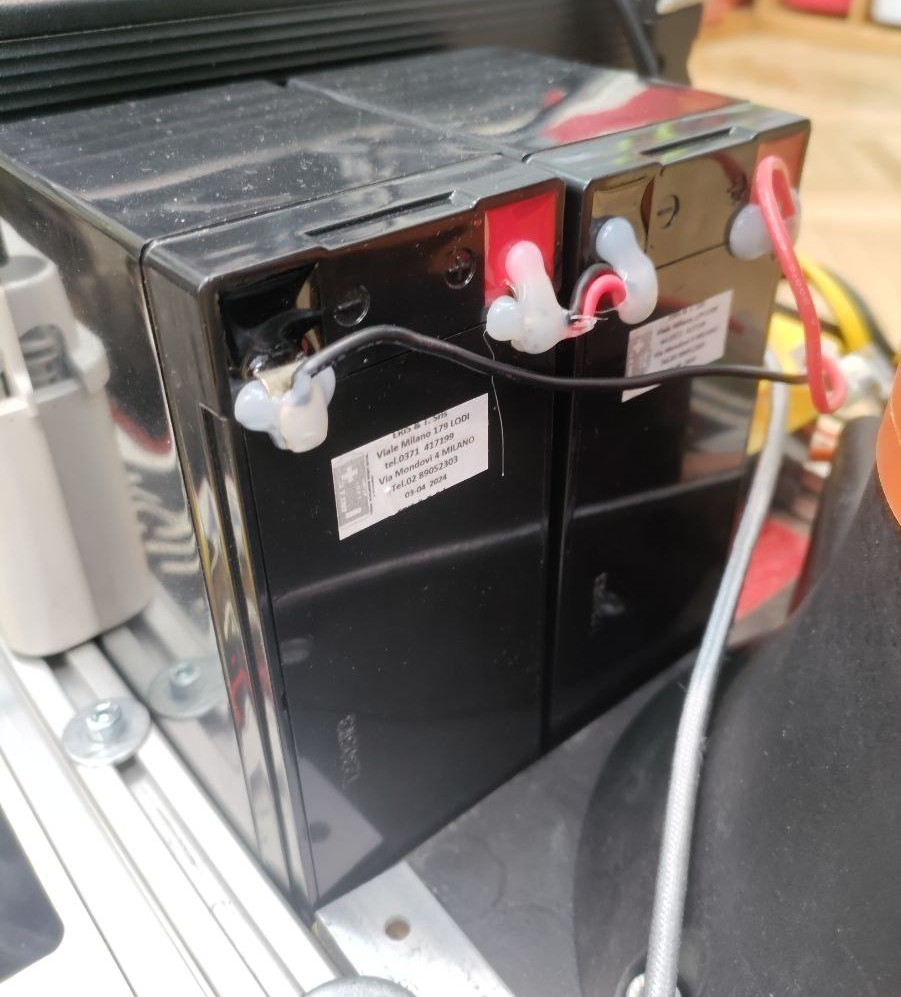
\includegraphics[width=0.5\textwidth]{c3_15.jpg}
    \captionsetup{width=1\linewidth}
    \caption{Lead batteries mounted onboard for the cobot and pneumatic pump}.
    \label{fig:c3_img15}
\end{figure}

% Add image of DC/DC converters
\begin{figure}[t]
    \centering
    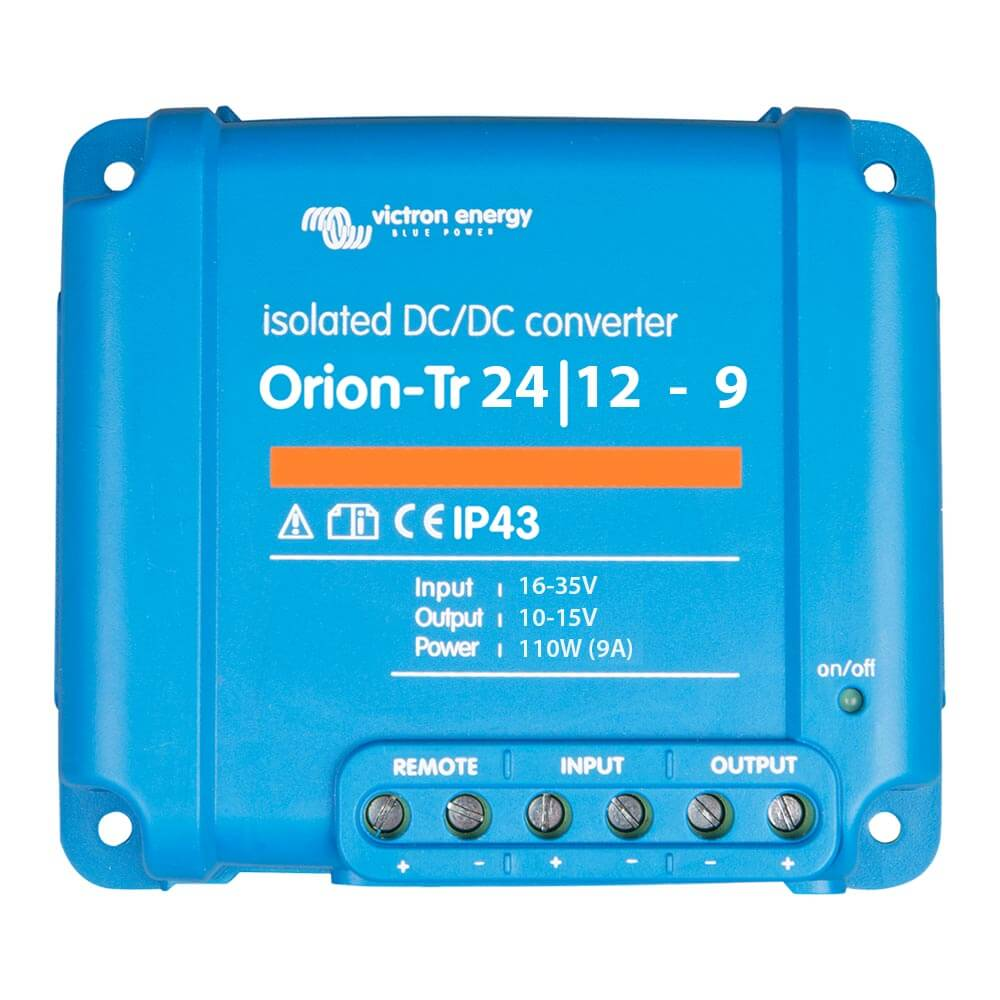
\includegraphics[width=0.4\textwidth]{chapter3_03.jpg}
    \captionsetup{width=1\linewidth}
    \caption{DC/DC converter used to power the robot's sensors and computer}.
    \label{fig:c3_img03}
\end{figure}

Another tool used to power the robots is a \textit{Santino}, a holy figure card presenting \textit{Saint Staianet}, 
the patron saint and protector of the mobile manipulation robot. This figure, placed in the front, as shown in \ref{fig:c3_img19},
helped and protected the robot during the development and testing of the project, ensuring that everything
was working fine and smoothly. The Santino was also used to provide a spiritual and religious touch to the project,
ensuring that the robot was blessed and protected during its missions.

\begin{figure}[t]
    \centering
    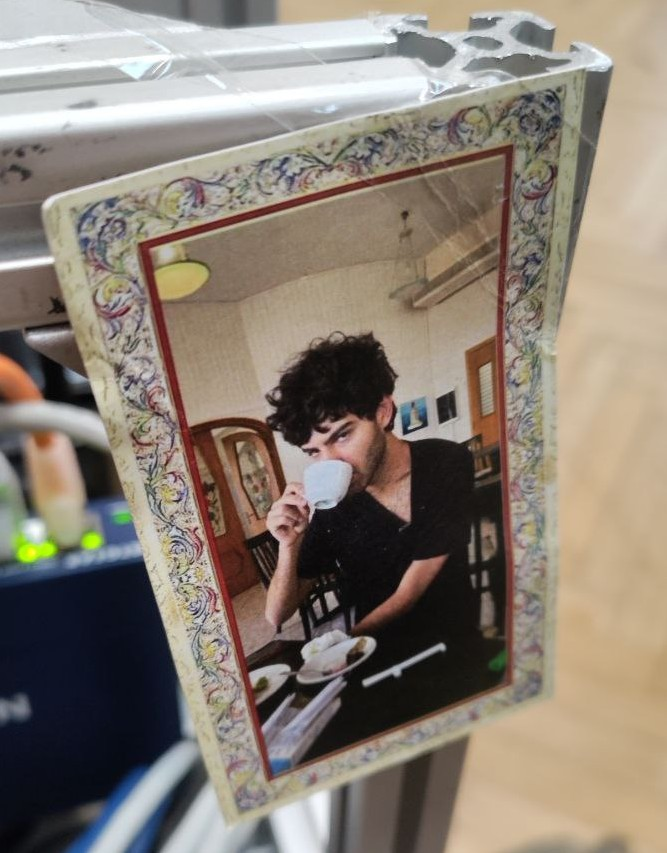
\includegraphics[width=0.5\textwidth]{c3_19.jpg}
    \captionsetup{width=1\linewidth}
    \caption{Santino}.
    \label{fig:c3_img19}
\end{figure}

\section{Complete Mobile Manipulation Setup}

Figures \ref{fig:c3_img28} and \ref{fig:c3_img29} show the complete mobile manipulation setup, with the robotic arm
mounted on top of the SCOUT 2.0 robot, and the soft gripper mounted on the robotic arm's end effector.
The setup is ready for the "soft grasping" demos, where the robot is tasked with grasping and manipulating objects
in simulated agricultural environments.

\begin{figure}[t]
    \centering
    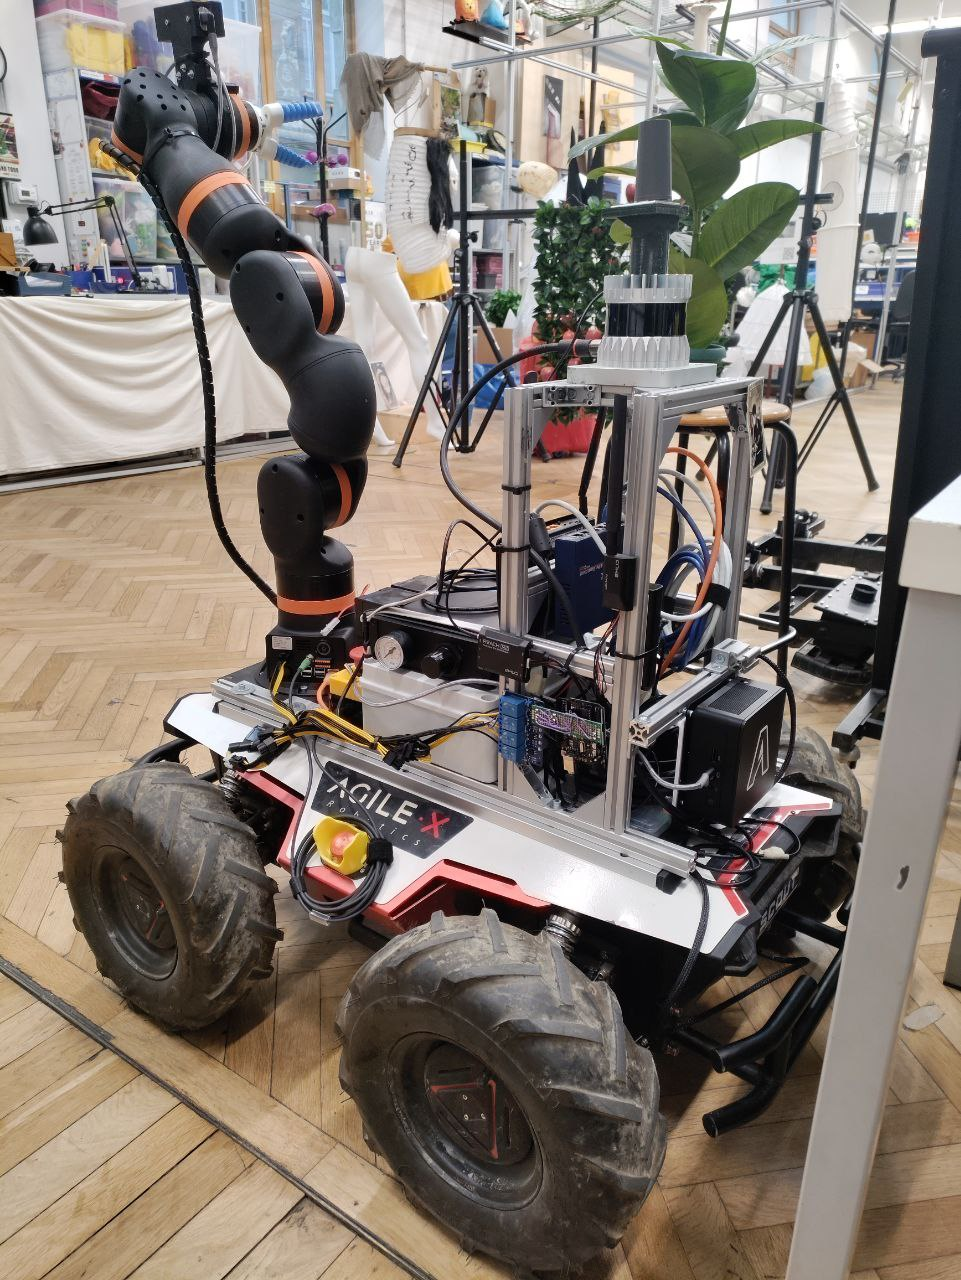
\includegraphics[width=0.8\textwidth]{c3_29.jpg}
    \captionsetup{width=1\linewidth}
    \caption{Front view of the robots}.
    \label{fig:c3_img29}
\end{figure}

\begin{figure}[t]
    \centering
    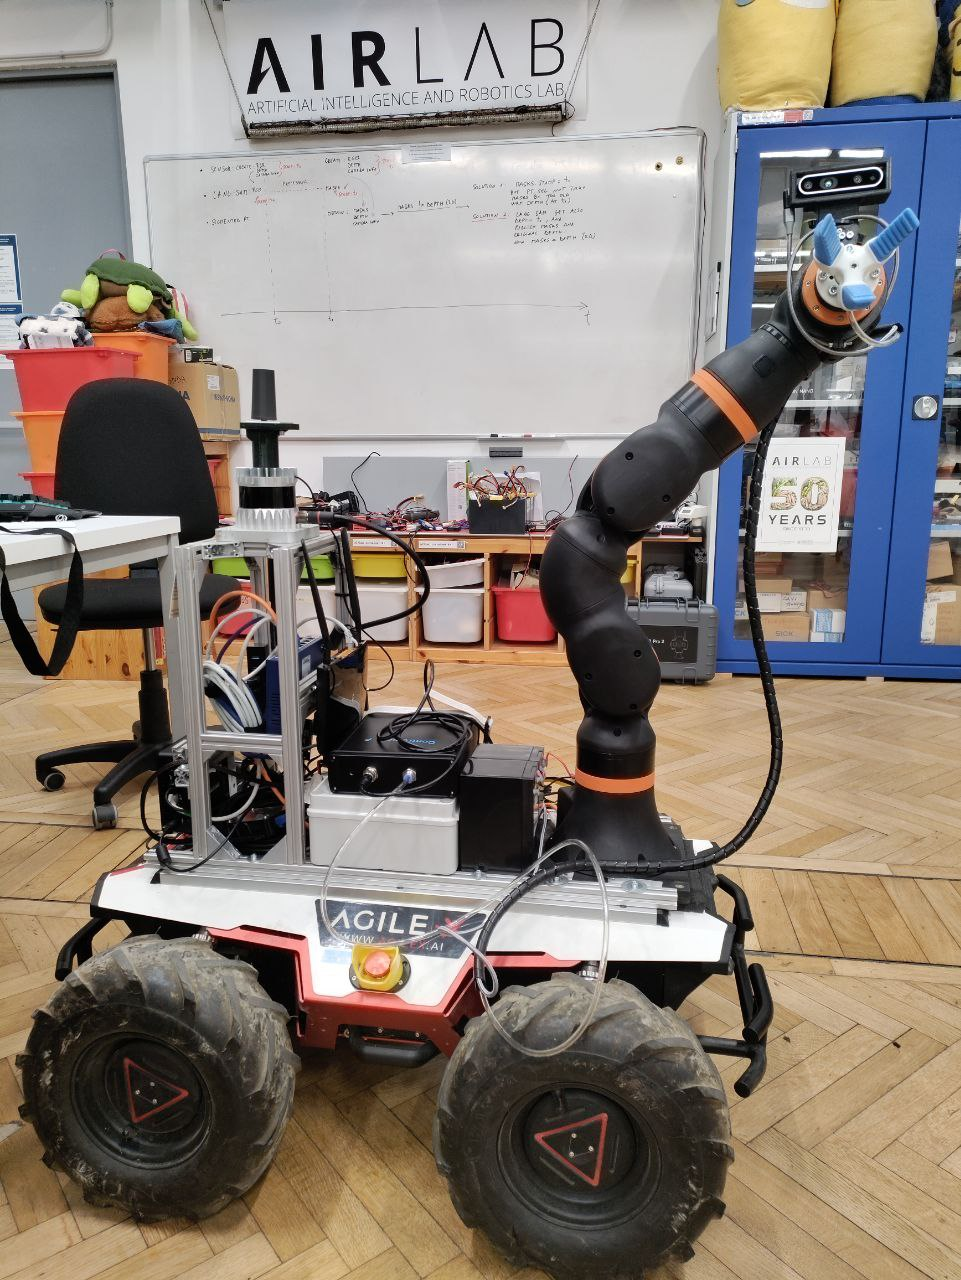
\includegraphics[width=0.8\textwidth]{c3_28.jpg}
    \captionsetup{width=1\linewidth}
    \caption{Lateral view of the robots}.
    \label{fig:c3_img28}
\end{figure}

\chapter{Software Architecture and Simulation Environments}

This chapter discusses the software architecture of the mobile manipulation robotic system and the simulation 
environments used for testing and development. The software architecture is based on the Robot Operating System 2 (ROS2)
middleware, which provides a flexible and modular framework for developing robotic applications. 
The simulation environments are based on Rviz2 and Ignition Gazebo, which provide realistic simulation environments
for testing the algorithms before deployment on the real robots.

\section{ROS2 Control Interface for Igus Rebel Arm}

The first step in developing the software architecture for the mobile manipulation robotic system is to interface the
Igus Rebel Arm with ROS2. The Igus Rebel Arm is a 6-DOF robotic arm that can be controlled by either the CAN binary bus
or the Ethernet interface (proprietary CRI protocol). The CAN bus interface is used for low-level access to the arm's
joints, while the Ethernet interface is used for high-level control and monitoring of the arm's state. 
The ROS2 control interface for the CAN bus was already implemented by the manufacturer \textit{Commonplace Robotics},
but the requirement was the development of a ROS2 control interface for the Ethernet interface since the CAN bus interface
requires a proprietary cable, which is not available to me. Using the Ethernet interface makes it easier to 
plug it into the switch and control the arm from any computer on the local network.

Developing the \textbf{ROS2 control interface} for the Ethernet interface required understanding the CRI protocol, which
is a protocol based on string messages. The CRI protocol is used to send commands to the arm in the form of
joint positions or velocities (jogs) and to receive feedback from the arm in the form of joint positions.
Controlling the cobot using ROS2 requires a hardware interface, used to command and control the robot by interfacing
with the hardware via the \textbf{CRI protocol}. The hardware interface is implemented as a ROS2 lifecycle node that
is interfaced directly with the Joint Trajectory Controller, which is a ROS2 controller that can be used to
control the arm using joint trajectory messages. This controller is then handled by MoveIt2, which is a ROS2
motion planning framework that can be used to plan and execute trajectories for the arm \cite{moveit2}.

%Add a figure of the control architecture
\begin{figure}[t]
    \centering
    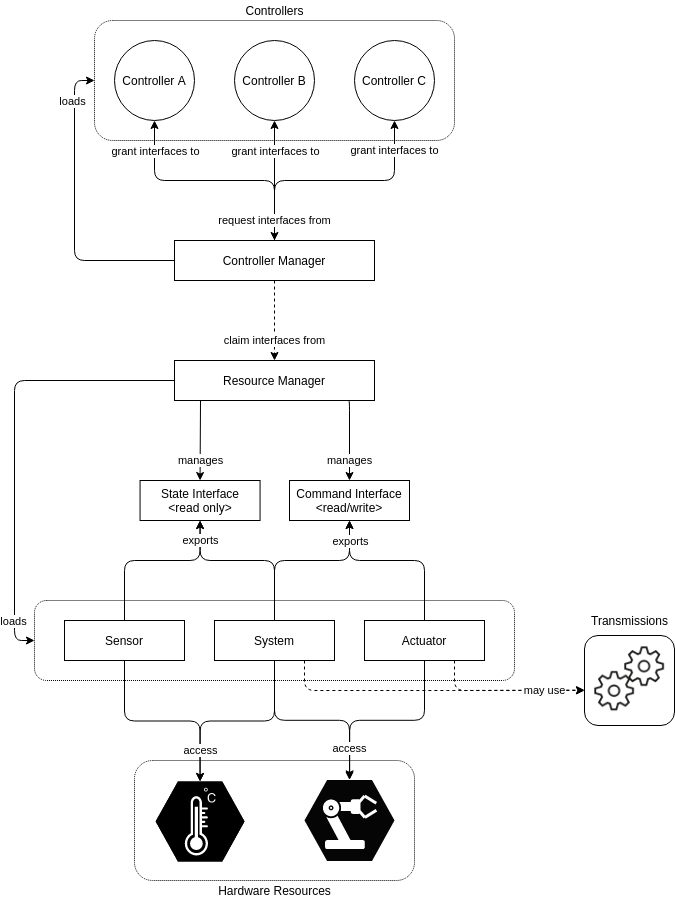
\includegraphics[width=0.6\textwidth]{c4_04.png}
    \caption{ROS2-Control Architecture example}
    \label{fig:ros2control}
\end{figure}

The diagram in figure \ref{fig:ros2control} shows an overview of how \textit{ROS2-Control} works.
The hardware interface implemented for controlling the Igus ReBel arm is a ROS2 lifecycle \textit{System Interface},
which is a type of interface that supports joints and actuators. The system interface accesses the hardware
via the CRI protocol and is managed by the \textit{Controller Manager} and the \textit{Resource Manager}. The
controller manager employed is provided by MoveIt2, in order to handle the cooperation between the hardware
interface and the joint trajectory controller, which receives the computed trajectories from MoveIt2.

\subsection{Joint Trajectory Controller}

The Joint Trajectory Controller is a ROS2 controller that can be used to control the arm using joint trajectory messages.
These messages are joint-space trajectories on a group of joints.
The controller interpolates in time between the points so that their distance can be arbitrary. 
Trajectories are specified as a set of waypoints to be reached at specific time instants, which the controller 
attempts to execute as well as the mechanism allows. Waypoints consist of positions, and optionally velocities and accelerations.

It can be operated either in position, velocity, or acceleration mode, depending on the type of trajectory message
that it handles.
The position mode is used to send joint positions to the arm, while the velocity mode is used to send joint velocities
in the form of jog values (velocities in percentage of the maximum velocity). The Joint Trajectory Controller can
be operated either in closed-loop or open-loop mode, depending on the type of feedback that is used to control the arm.
In closed-loop mode, the controller uses the joint positions received from the arm as feedback to adjust the trajectory
to the desired position, by controlling the arm via velocity commands. In open-loop mode, the controller sends the
trajectory to the arm without any feedback, which can be useful for testing the arm's performance without any feedback
control. The closed-loop velocity control requires a PID controller to adjust the velocity commands based on the
difference between the desired and actual joint positions. The PID controller requires tuning the gains to
achieve the desired performance of the arm. I did not manage to find the best gains for the PID controller,
for a stable and smooth trajectory execution, so I used the open-loop mode for controlling the arm.

MoveIt controller managers, somewhat a misnomer, are the interfaces to your custom low-level controllers. 
A better way to think of them is controller interfaces. The included \textit{MoveItSimpleControllerManager} is sufficient
for the robot controllers that provide ROS2 actions for \textit{FollowJointTrajectory}.

\section{MoveIt2 and RViz2 Simulation Environment}

% Add a figure of the MoveIt2
\begin{figure}[t]
    \centering
    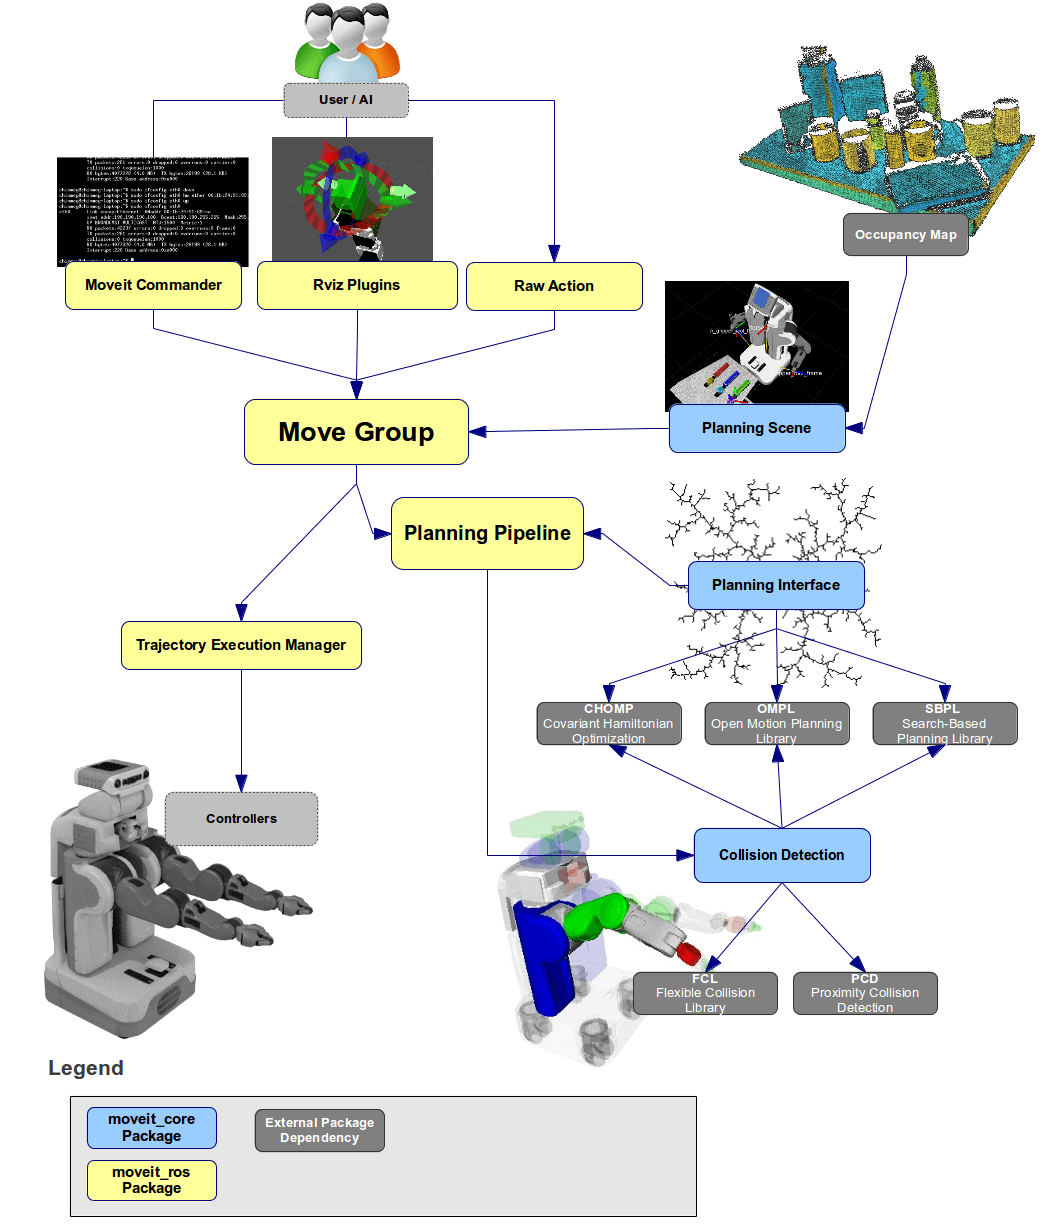
\includegraphics[width=0.8\textwidth]{c4_01.png}
    \caption{MoveIt2 General Architecture}
    \label{fig:moveit2}
\end{figure}

%Add a figure of the control architecture
\begin{figure}[t]
    \centering
    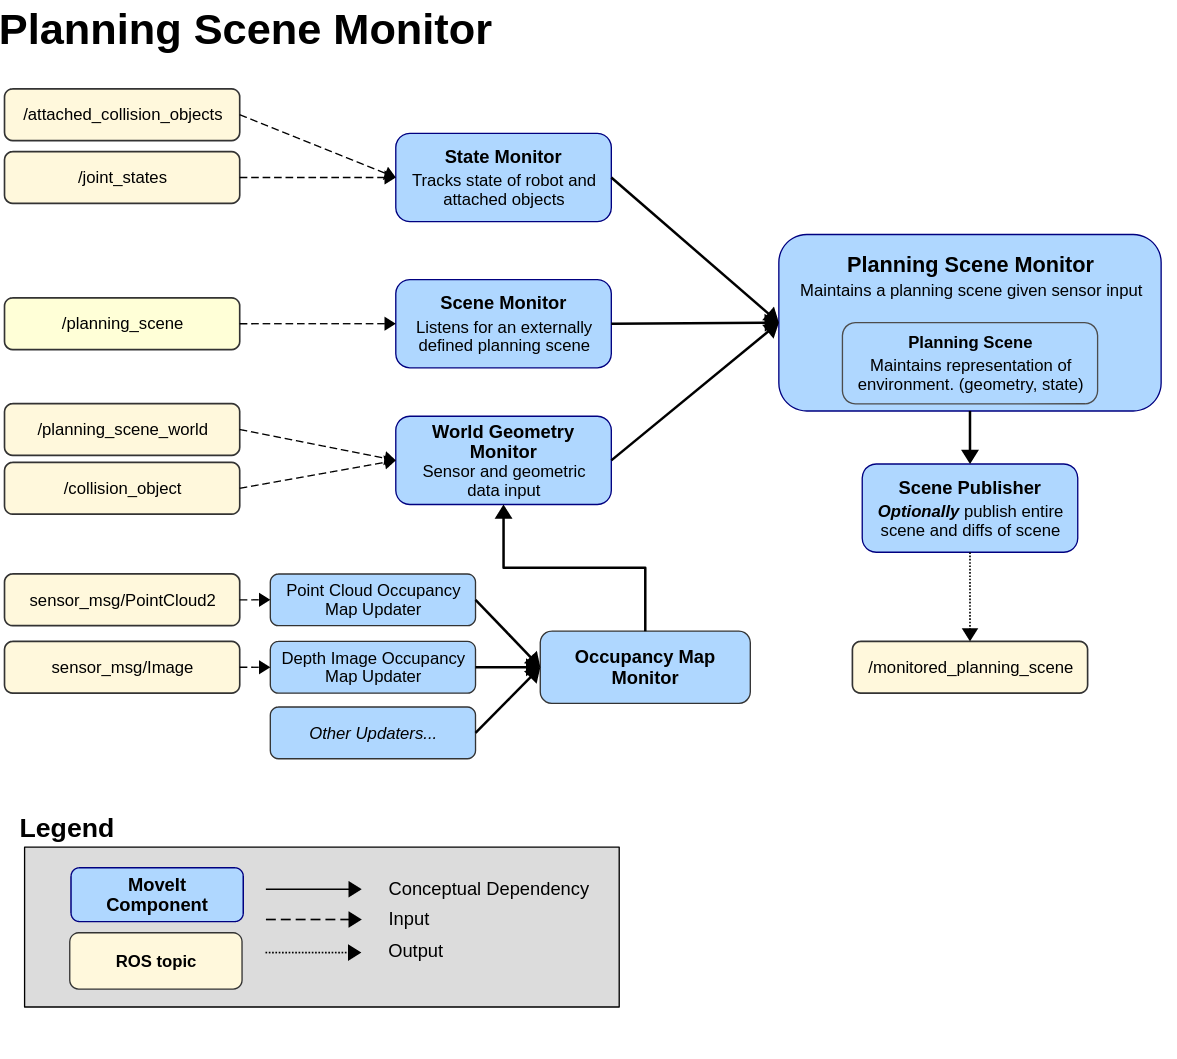
\includegraphics[width=0.8\textwidth]{c4_03.png}
    \caption{Planning Scene and Occupancy Mapping Architecture}
    \label{fig:planninscence}
\end{figure}


MoveIt2 is a ROS2 framework that provides a set of tools for motion planning, kinematics, control, perception, and
manipulation. It is a powerful tool for controlling robotic arms and mobile bases, and it can be used to plan and
execute trajectories for the arm. MoveIt2 is based on the ROS2 middleware and provides a flexible and modular
framework for developing robotic applications.

The figure \ref{fig:moveit2} shows the general \textbf{architecture of MoveIt2}. The MoveIt2 framework consists of several
components, including the Planning Scene, the Planning Pipeline libraries, the Kinematics Solver, the Collision
Checker, the Trajectory Execution Manager, and the Occupancy Mapping tools.
The Planning Scene is a representation of the robot's environment, including the robot's state, the obstacles in the
environment, and the robot's kinematic model. The diagram in figure \ref{fig:planninscence} shows the architecture
of the Planning Scene and the modules with which it interacts.
The Planning Pipeline libraries are used to generate motion plans
for the robot, using the robot's kinematic model and the obstacles in the environment. The Kinematics Solver is
used to compute the robot's joint positions for a given end-effector pose, using the inverse kinematics
computations based on the robot's kinematic model. The Collision Checker is used to check for collisions between
the robot and the obstacles in the environment, using the robot's kinematic model and the obstacles' geometries.
The Trajectory Execution Manager is used to execute the motion plans generated by the Planning Pipeline libraries,
using the robot's joint positions and velocities. The Occupancy Mapping tools are used to generate volumetric 3D 
occupancy maps of the surrounding environment, using depth perception sensors to construct a map
of the obstacles in the environment. 

\begin{figure}[t]
    \centering
    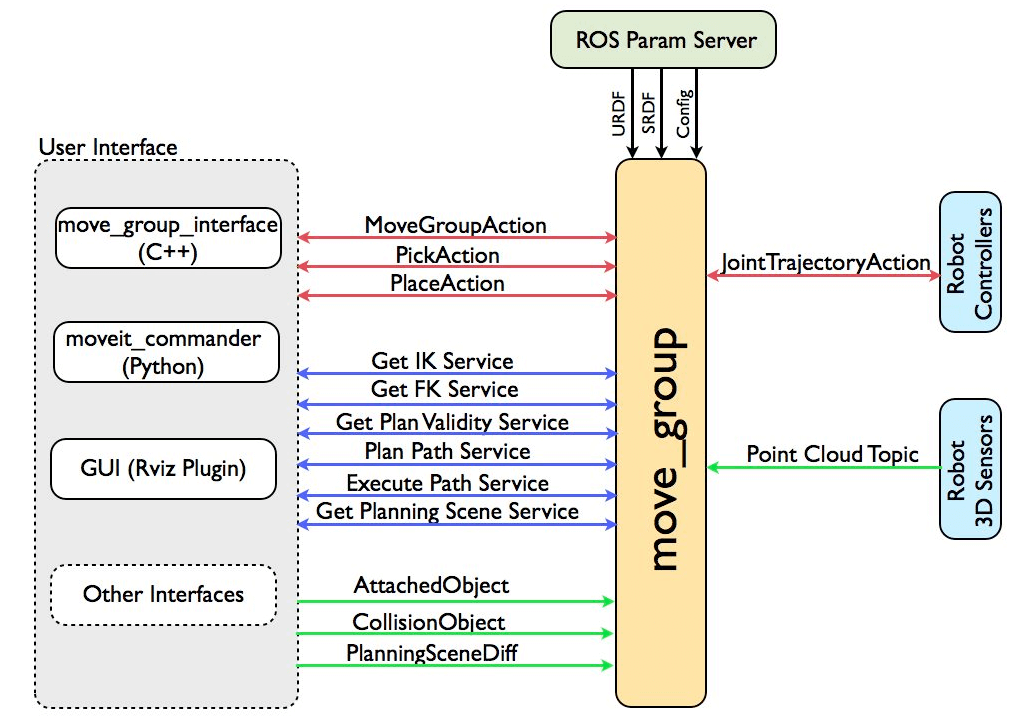
\includegraphics[width=0.8\textwidth]{c4_02.png}
    \caption{MoveGroup Interface}
    \label{fig:move_group}
\end{figure}

MoveIt2 provides the \textit{MoveGroupInterface} class, which is a high-level interface to the MoveGroup node, which is the
class that provides a set of methods for controlling the robot's motion planning and execution. 
Figure \ref{fig:move_group} shows the architecture and the modules with which it interacts.
The \textit{MoveGroupInterface} provides also methods for interacting with the robot's planning scene, 
including adding and removing obstacles, setting the robot's state, and setting the robot's end-effector pose. 
The \textit{MoveGroupInterface} can be used to plan and execute trajectories for the robot. 
It allows to define and compute joint-space goals, Cartesian-space goals,
and pose goals for the robot's end-effector, which is used to compute the joint space trajectories.

% Add a figure of the rviz2 interface with moveit2
\begin{figure}[t]
    \centering
    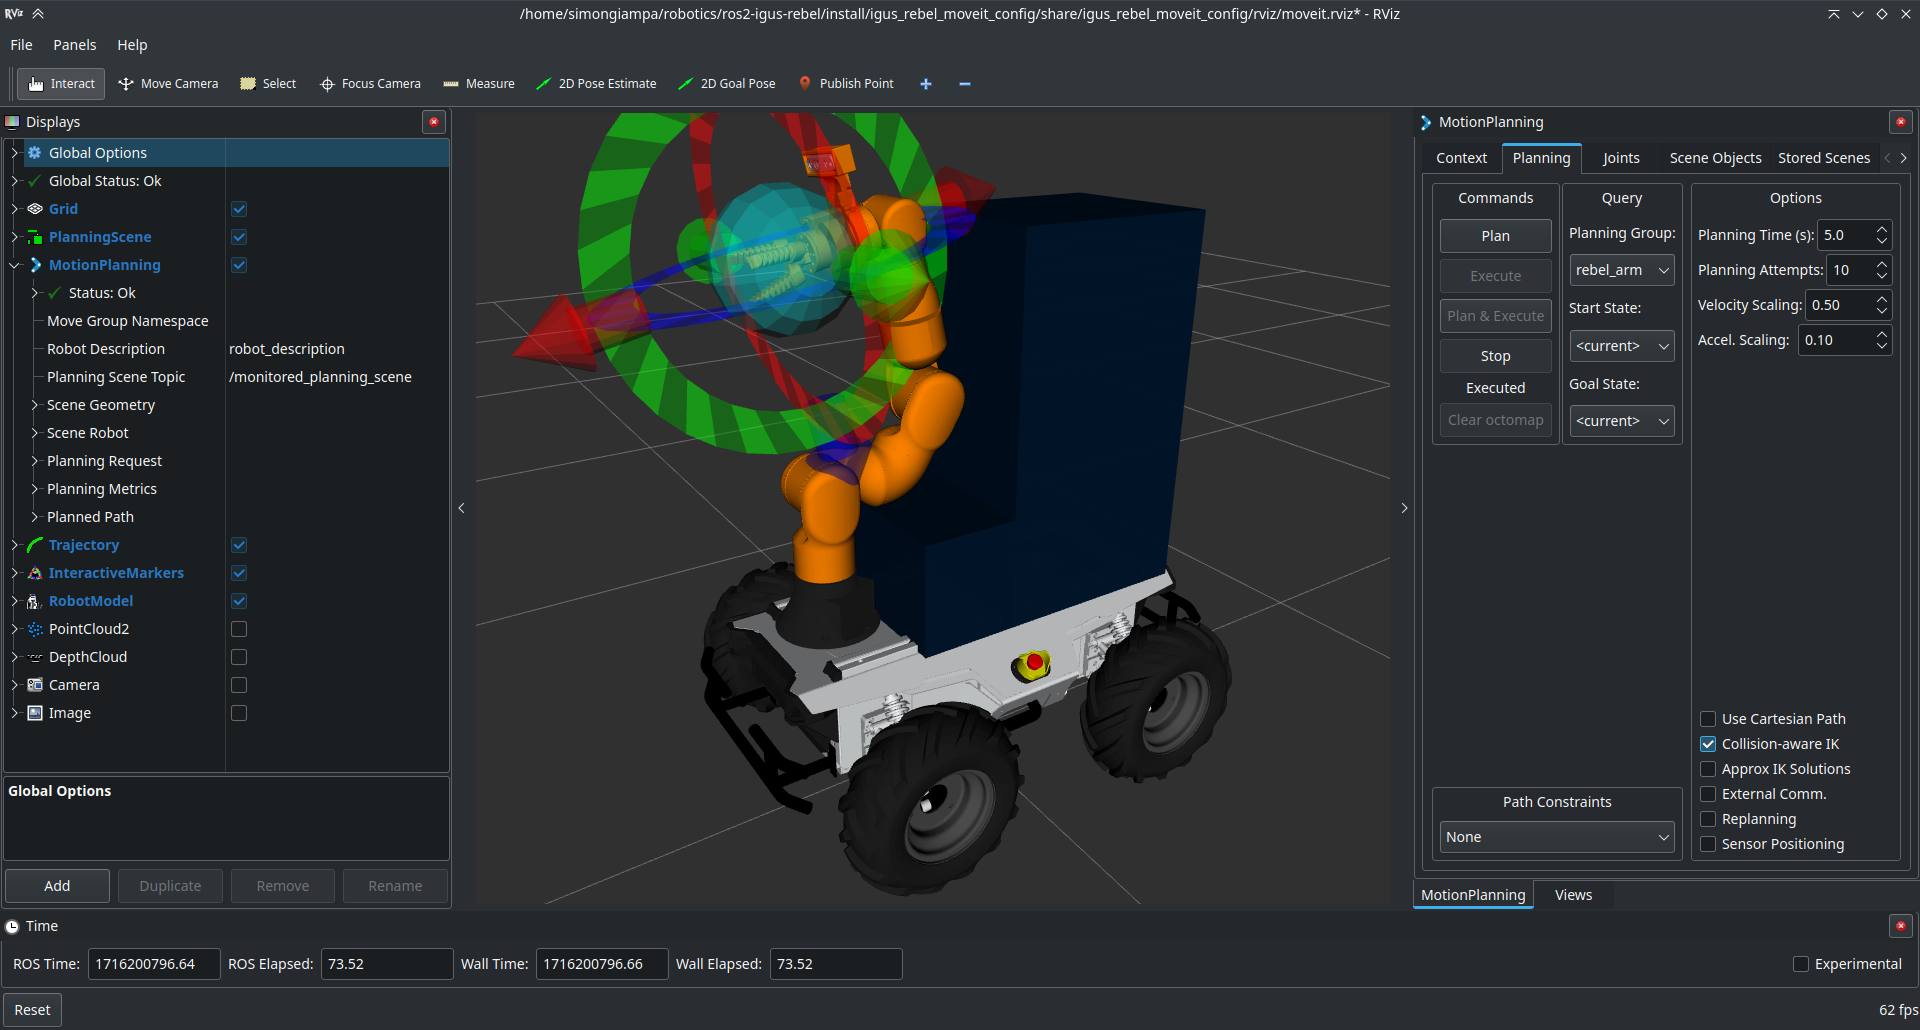
\includegraphics[width=1.0\textwidth]{c4_11.png}
    \caption{RViz2 Interface with MoveIt2 Control Panels and the mobile manipulation robot.}
    \label{fig:rviz2}
\end{figure}


MoveIt2 can be used along with RViz2, which is a 3D visualization tool for ROS2 that can be used to visualize the
robot's motion in both simulated and real environments. RViz2 provides a set of tools for visualizing the robot's
kinematic model, the robot's state, the obstacles in the environment, and the robot's motion plans.
Figure \ref{fig:rviz2} shows a screenshot of the RViz2 interface with the control panels dedicated to the MoveIt2
planning and execution tools. The figure shows the Igus Rebel cobot mounted on the Scout mobile robot,
with blue collision boxes to prevent the arm from colliding with the sensors mounted on top.
With this interface, it is possible to send joint space goals to the robot
and control it via the underlying hardware interface. There is also an interactive marker that allows the user
to set the robot's end-effector pose by dragging it around in the RViz2 interface.

I developed a custom library that incorporates the \textit{MoveGroupInterface}, providing high-level functions
in C++ that allow to plan and execute different types of motion, as well as computing the end-effector position
and orientation quaternion from sensor input data. This library makes use of different planners to obtain
the highest probability of generating a valid motion trajectory given the planning scene, and current and target
joint positions. The planner \textit{Pilz Industrial Motion Planner} is used for linear cartesian trajectories 
since it outperforms the other planners for this task. The \textit{OMPL} (Open Motion Planning Library) and
\textit{STOMP} (Stochastic Trajectory Optimization) motion planners
are instead used for generating trajectories with joint-space or cartesian-space targets.
The kinematic solver used throughout the project is \textit{KDL} (Kinematics and Dynamics Library), which is a C++ library
that provides a set of tools for computing the forward and inverse kinematics of the robot's kinematic model.
For collision detection, the \textit{FCL} (Flexible Collision Library) is used, which is a C++ library that provides
a set of tools for detecting collisions between the robot and the obstacles in the environment.
Its advantage is the integration with Octomap for 3D collision checking, which is used in the MoveIt2 framework.

\section{Robotic Arm Visual Servoing}

The MoveIt2 library provides also a framework for visual servo-ing, which is a technique used to control the robot's
end-effector pose using visual feedback from a camera. The visual servo-ing framework in MoveIt2 is based on the
\textit{MoveItServo} package, which provides a set of tools for controlling the robot's end-effector pose using
servo-ing algorithms. The servo-ing algorithms are used to compute the robot's joint positions for a given end-effector
pose. I developed the code to integrate these tools with the camera visual feedback, in order to perform visual servo-ing
experiments with the Igus Rebel Arm. 

The servo-ing algorithms provided by MoveIt2 allow also for \textbf{real-time control and teleoperation} of the robot arm's
end-effector pose. The teleoperation allows the user to control the robot's end-effector pose using a joystick controller.
The real-time control allows the user to control the robot's end-effector pose using camera visual feedback
in real-time without pre-computing the joint trajectories. Realtime control is useful for controlling the robot's
end-effector pose in dynamic environments, where the obstacles are moving and the robot needs to adapt to the changes
in the environment.

\begin{figure}[t]
    \centering
    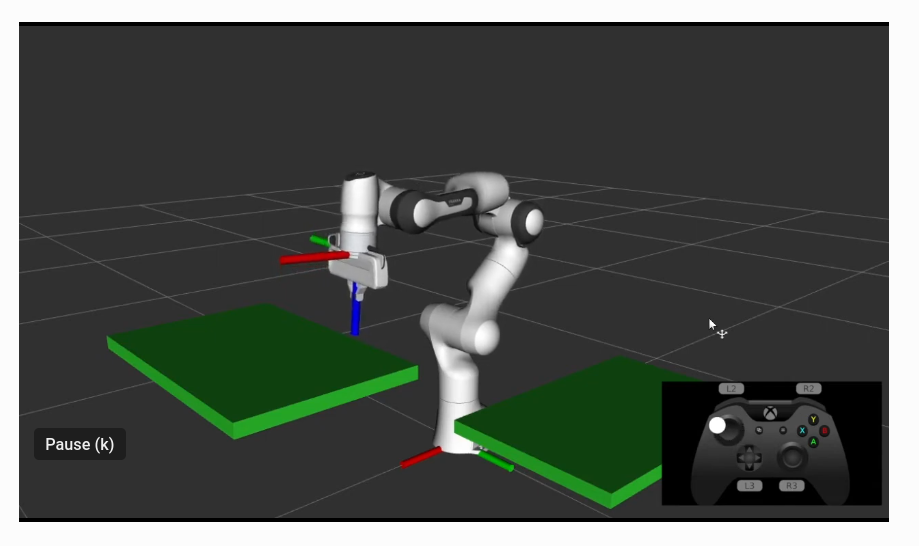
\includegraphics[width=0.8\textwidth]{c4_05.png}
    \caption{Teleoperation with a joystick controller in RViz2 with the Franka Emika Panda}
    \label{fig:teleop}
\end{figure}


After many trials and errors, I managed to get the \textbf{visual servo-ing} working
only with input cartesian poses close to the initial pose of the arm. The servoing algorithm requires
a good initial guess of the end-effector pose, in order to converge to the desired pose.
Since I tested the visual servo-ing with the arm in the open-loop mode, the servo-ing algorithm was not able to
compensate for the errors in the joint positions, which led to the arm not reaching the desired pose.
Then I switched to the closed-loop mode, but the PID controller gains were not tuned properly, which led to strong
oscillations in the joint positions and the arm not reaching the desired pose stably. I did not manage to find the
best gains for the PID controller, so I had to abandon the visual servo-ing experiments with the arm.
The package is still available in the repository, but it is not used in the final implementation
of the mobile manipulation robotic system. Furthermore, the servo-ing algorithms using cartesian input poses
rely exclusively on ROS2-Iron distribution.

\section{Collision Avoidance with Octomap}

The MoveIt2 library provides a framework for collision avoidance using the \textbf{Octomap} library, which is a library for
generating volumetric 3D occupancy maps of the surrounding environment \cite{hornung13octomap}.
Octomap is a 3D probabilistic occupancy grid representation of the robot's environment. It divides the space into voxels
(3D cubes) and assigns probabilities to each voxel, indicating whether it's occupied (by an obstacle) or free.
MoveIt2 integrates data from various sensors, such as the depth camera to update the Octomap in real time.
Figure \ref{fig:octomap} shows the integration of Octomap inside MoveIt2, where the voxels defining the occupancy
mapping are inside the Planning Scene, so the motion planning algorithms can use the voxels to plan a trajectory
that avoids them.

MoveIt2's collision checker uses the Octomap to efficiently check for collisions between the robot's planned trajectory
and the environment. By checking if the voxels along the path are occupied, it can determine if the robot will collide 
with any obstacles. The probabilistic nature of Octomap helps deal with sensor noise and uncertainty. 
If a voxel has a high probability of being occupied, it's treated as an obstacle.

MoveIt2's motion planners, such as \textit{OMPL} (Open Motion Planning Library), use the Octomap
to generate collision-free paths. The planners avoid occupied voxels to ensure the robot's motion doesn't lead to collisions.
If the environment changes during execution (e.g., an obstacle moves), MoveIt2 can use the updated Octomap 
to quickly replan a new collision-free path, allowing for dynamic obstacle avoidance.
This allows for a dynamic representation of the environment, even if obstacles move.

% Add a screenshot of the Octomap in RViz2
\begin{figure}[t]
    \centering
    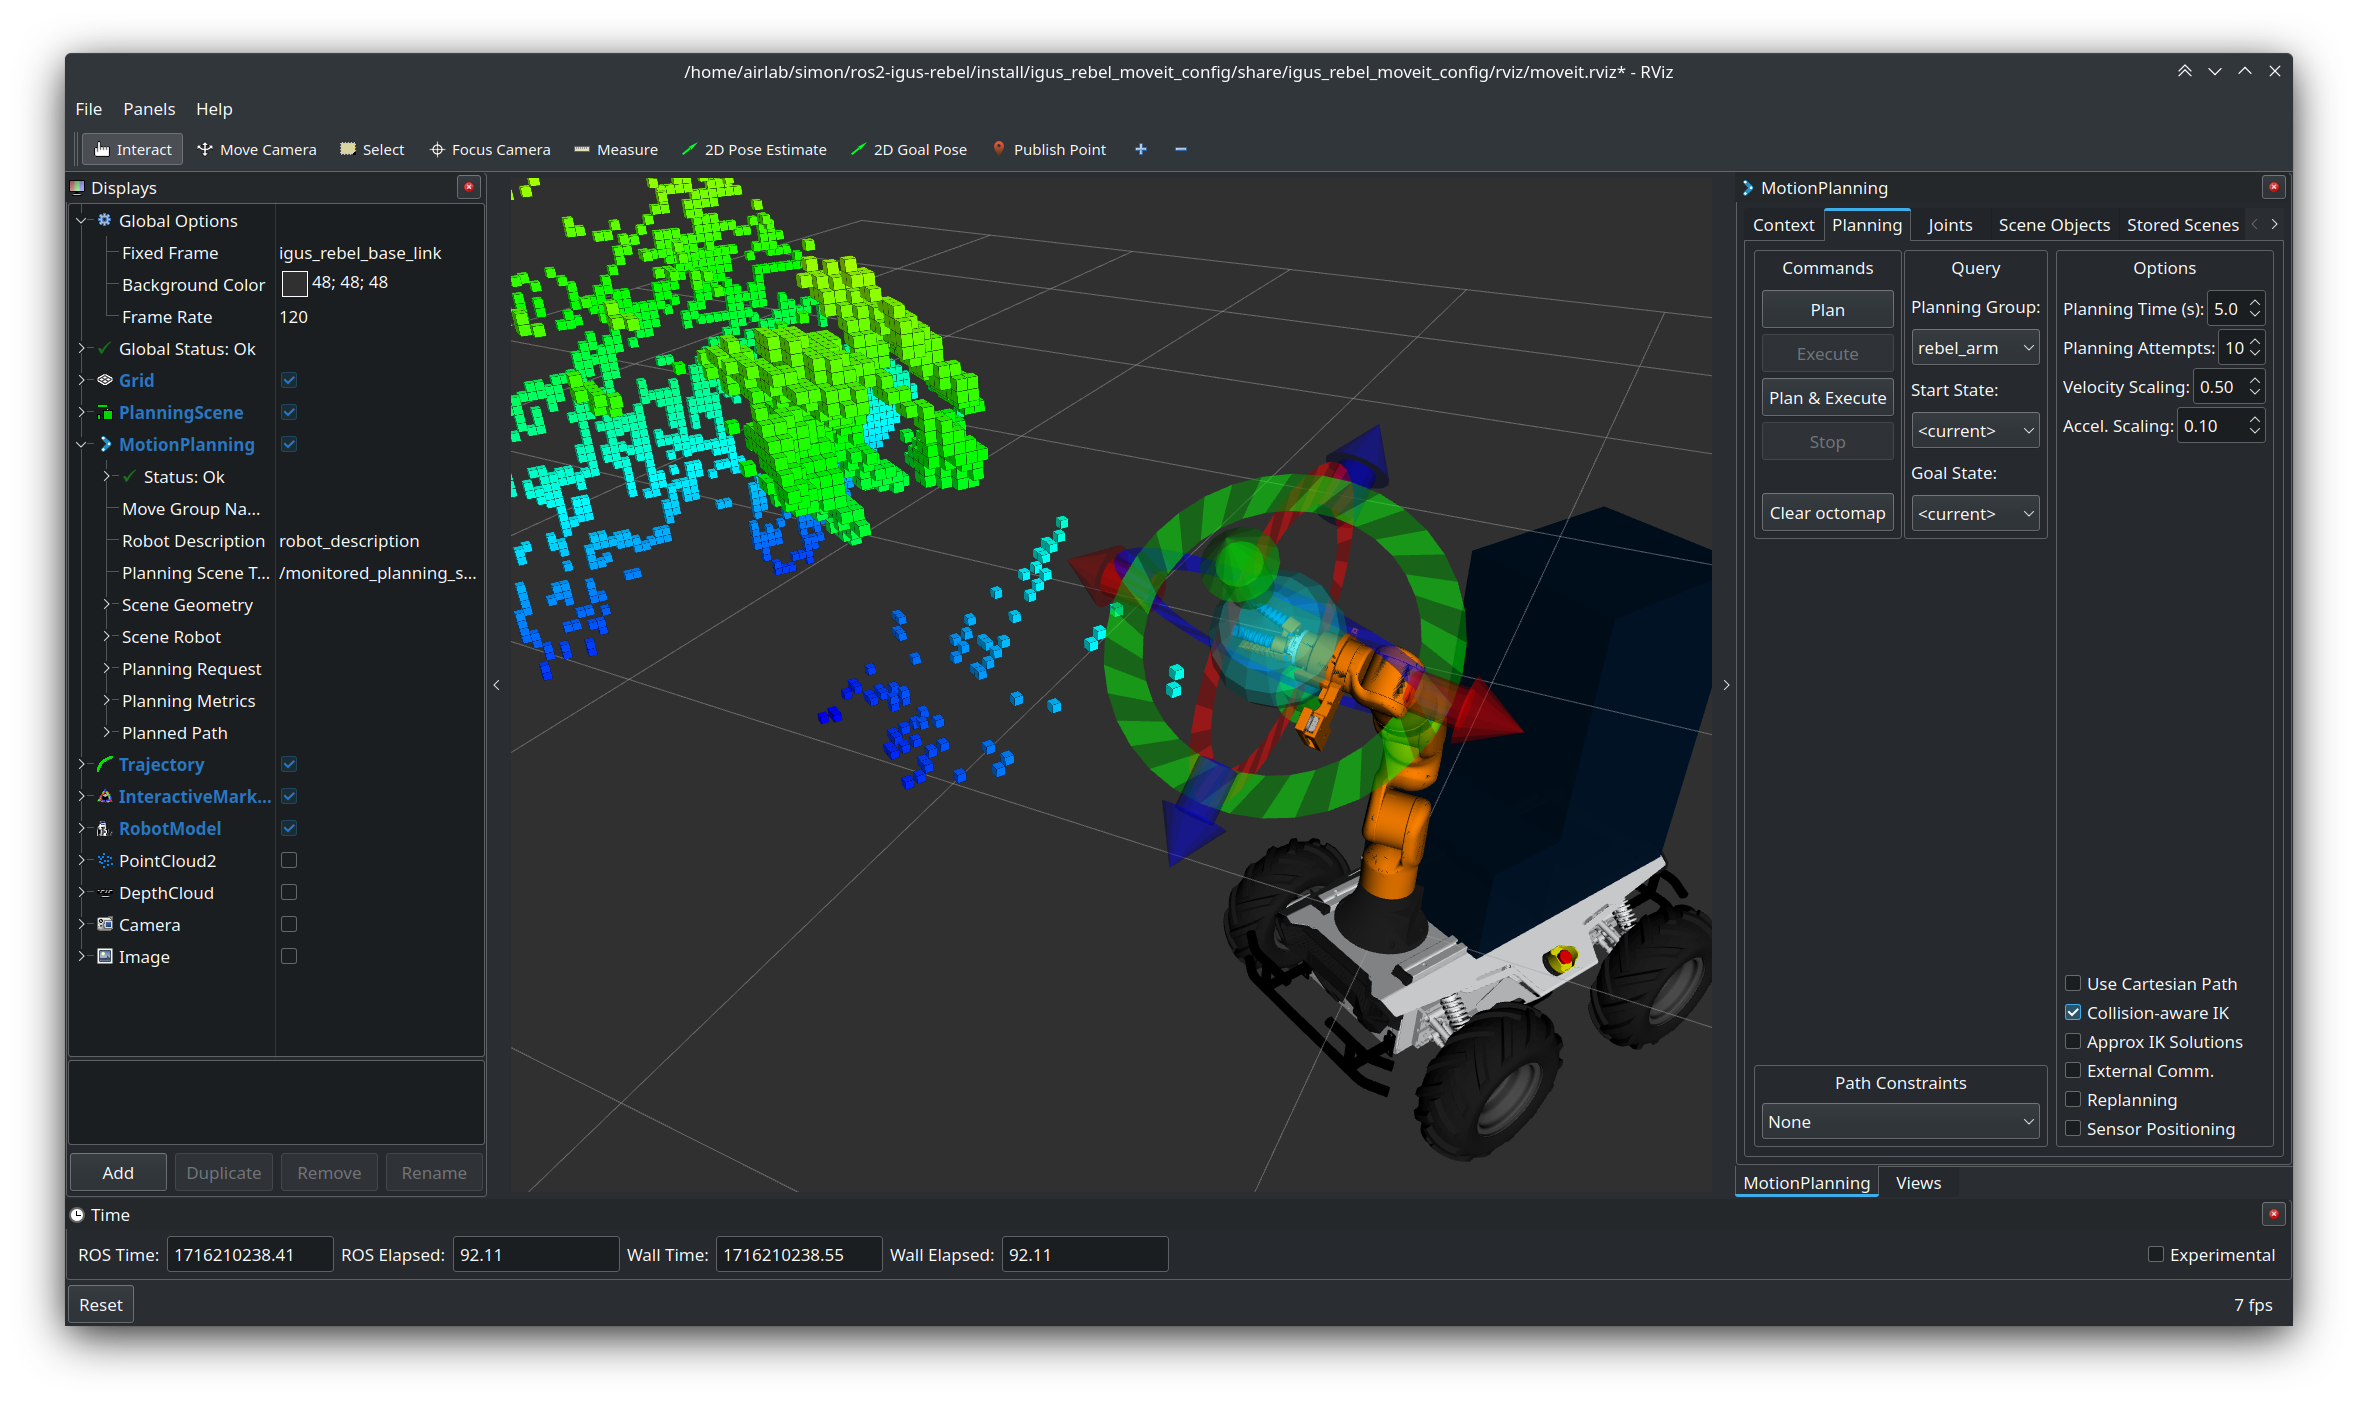
\includegraphics[width=1.0\textwidth]{c4_15.png}
    \caption{Mobile robot using the depth camera to construct the Octomap with the obstacles nearby}
    \label{fig:octomap}
\end{figure}

However, the reality is far from the ideal scenario. The Octomap library is not yet fully integrated with the MoveIt2
interfaces, resulting in a \textbf{poorly optimized} Octomap probabilistic representation of the environment.
In fact, the library takes track of the free space as well as the occupied space, resulting in a memory and computationally
intensive update process, meaning that the time taken for each Octomap update is very high. The Octomap
library for ROS2 is a porting of its ROS1 counterpart, which is fully functional but still lacks some features.
One of the features that are missing is the ability to update the Octomap in realtime when part of the
environment changes. In the current version of the software, Octomap will only update a few voxels around the
part of the environment that changed, without fully removing the voxels corresponding to the obstacle that moved
and that is not present in the scene anymore. This leads to \textbf{false positives in the collision checking}, which
prevents the robot from executing the planned trajectory. This feature is critical for dynamic obstacle avoidance
because the robot needs to avoid the voxels corresponding to the obstacles and touch the voxels corresponding
to the object that the end effector needs to grasp. This means that not only does the robot need to avoid the obstacles
but also understand which voxels the robot arm can collide with.
The Octomap Library is still under development, and it is expected to be correctly integrated with MoveIt2 in the future.

\section{Soft Gripper Pneumatic Pump Actuation}

The soft gripper is actuated using a ROS2-control interface that acts as a hardware interface to the Arduino UNO
microcontroller that controls the pneumatic pump. The hardware interface works by providing a ROS2 service server that 
listens for commands to open or close the gripper and sends the corresponding commands to the Arduino UNO microcontroller
via serial communication. 
The serial communication handles with the UART protocol, which is used to send and receive string messages.
The serial data transfer is done using the \textit{thermios} library, which is a POSIX-compliant library for serial
communication in Linux, supporting the C language.

The Arduino UNO microcontroller is programmed to control the pneumatic pump by changing
the state of the relays connected to its digital pins. The Arduino UNO listens in the serial port for string commands
that it interprets as the pins to be set high or low, to open or close the gripper. The pneumatic pump is connected
to the Arduino UNO via a relay module with 4 relays, one for each digital pin of the pump. Two of which
are the VCC and GND pins, and the other two are the GRIP and RELEASE pins. The GRIP pin is used to close the gripper,
while the RELEASE pin is used to open the gripper.

\section{Autonomous Navigation with NAV2}

Nav2 is a powerful open-source software framework used for autonomous navigation within the ROS2 ecosystem
\cite{macenski2020nav2}.
It provides a comprehensive set of tools and algorithms for enabling robots to navigate complex environments intelligently.
With Nav2, robots can perceive their surroundings, localize themselves, plan optimal paths, and execute 
those paths while avoiding obstacles. Its modular architecture allows for customization and integration with various sensors,
such as LiDAR and cameras, making it adaptable to different robot platforms and use cases. 
Nav2's flexibility and robust features make it a popular choice for both research and industrial applications 
in fields like robotics and autonomous vehicles
\cite{macenski2023survey}.

Nav2's \textbf{modular architecture} enables the seamless integration of various plugins that contribute
to its robust autonomous navigation capabilities. Costmap plugins, such as static and obstacle layers,
create a real-time representation of the robot's environment, highlighting obstacles and free space. 
Collision monitors continuously assess the robot's planned path against this costmap ensuring safe navigation.
Localizers, like AMCL, estimate the robot's position within the environment, while mappers like SLAM create and update maps
of the surroundings. Planners, such as global planners (e.g., Hybrid A*) and local planners (e.g., DWB),
work in tandem to generate collision-free paths for the robot to follow, enabling efficient and fast navigation. 
Additionally, plugins like controllers and recovery behaviors further enhance Nav2's ability to handle unexpected
scenarios and ensure the robot reaches its goal.

Given these premises and features, I decided to use Nav2 as the primary navigation stack for the mobile manipulation
robotic system. The Nav2 stack is used to plan and execute trajectories for the mobile base, using the robot's
LiDAR sensor to perceive the environment and avoid obstacles. The stack operates within a ROS2 
composable node architecture, which allows for the integration of various plugins and algorithms to achieve
efficient intra-process communication and data sharing between the various components and threads of the stack.
I created and configured the Nav2 stack to work with the AgileX Scout robot, using the SLAM Toolbox algorithm
for creating maps of the laboratory. Figure \ref{fig:nav2_hallway} and figure \ref{fig:nav2_airlab} show the autonomous
navigation of the robot in the hallways and AIRlab in building 7 of Politecnico di Milano, respectively.

% Add screenshots of map and costmap in RViz2
\begin{figure}[t]
    \centering
    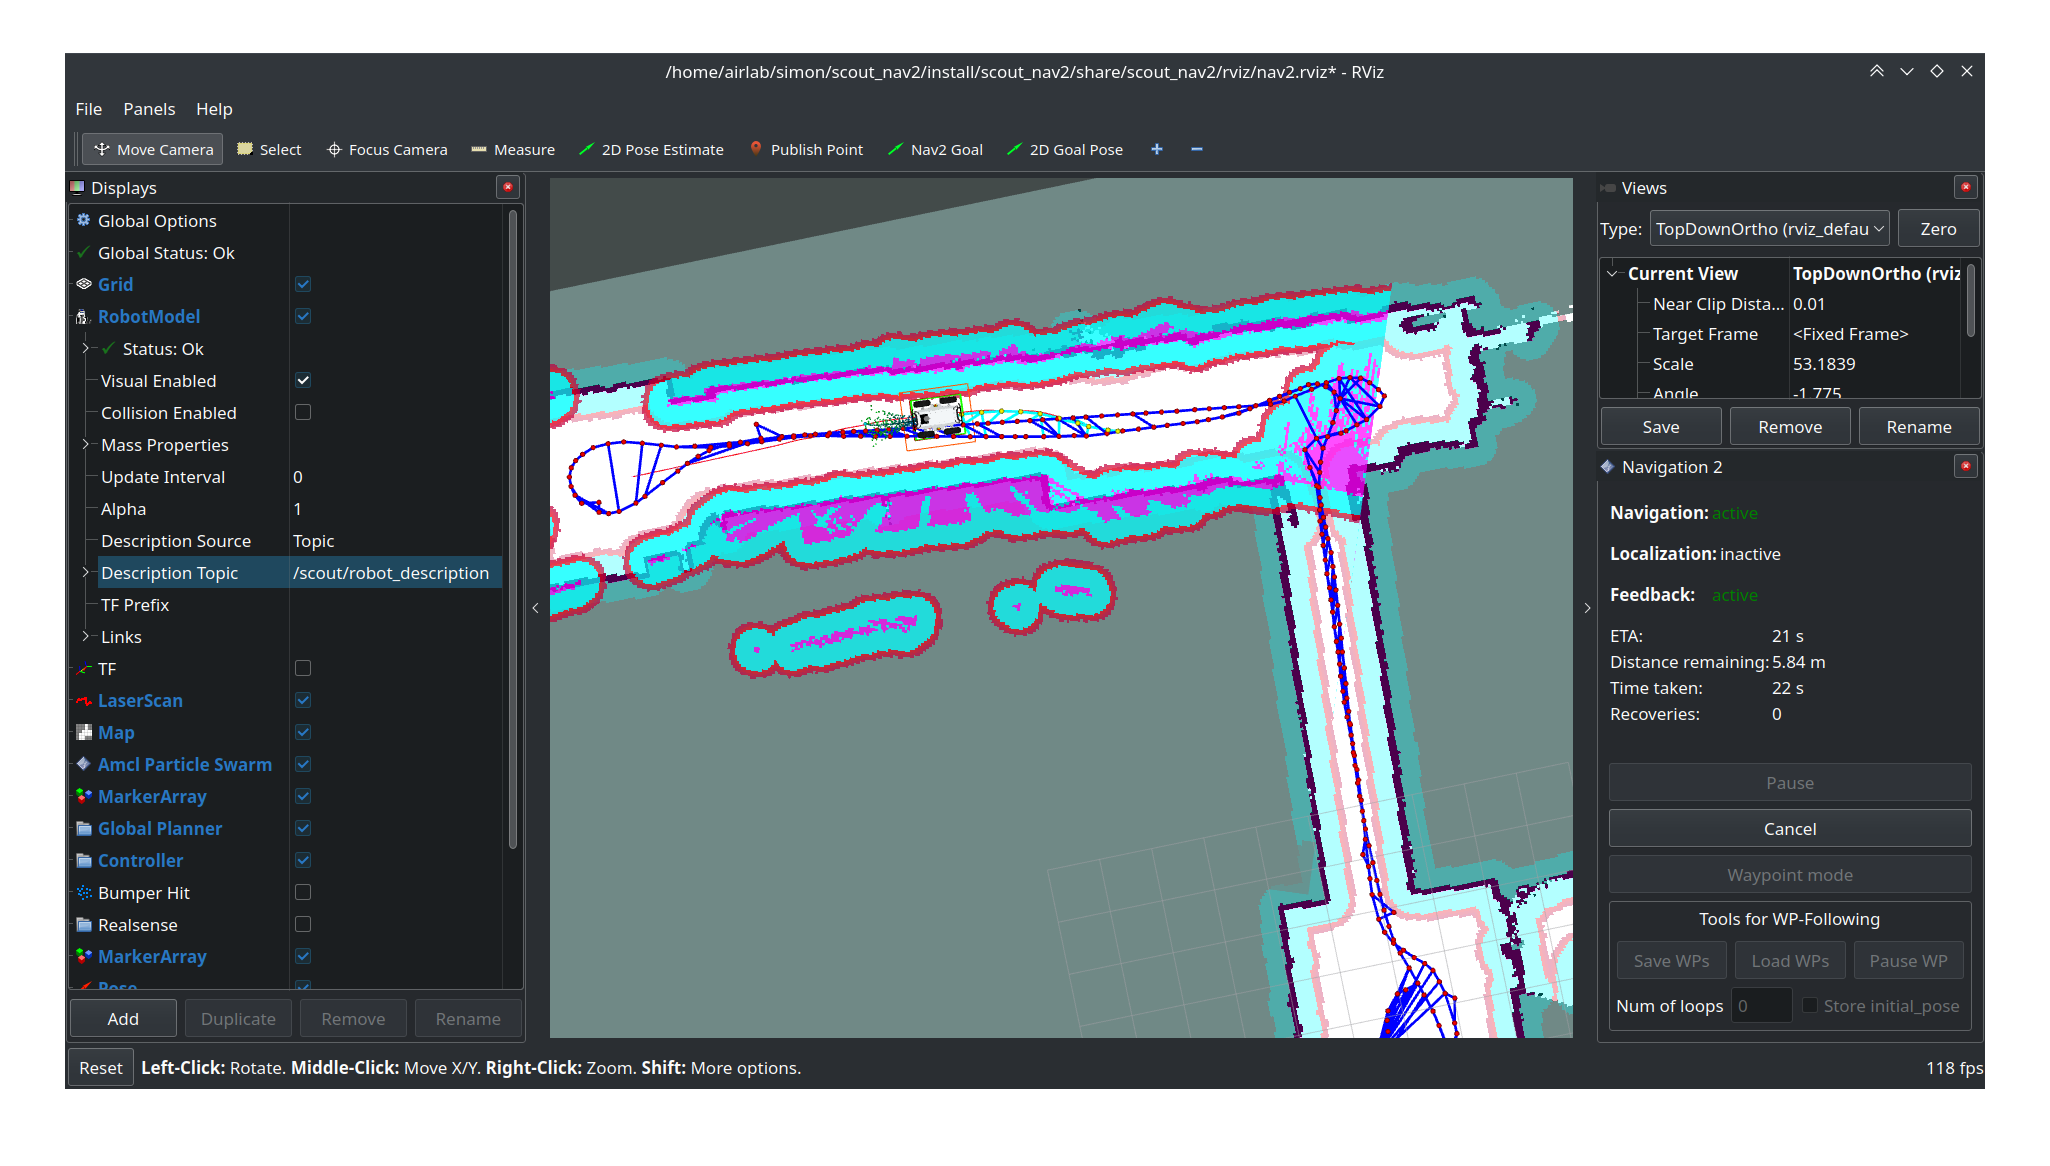
\includegraphics[width=1.0\textwidth]{c4_20.png}
    \caption{Autonomous Navigation with Nav2 in the hallways of building 7 of Politecnico di Milano}
    \label{fig:nav2_hallway}
\end{figure}

\begin{figure}[t]
    \centering
    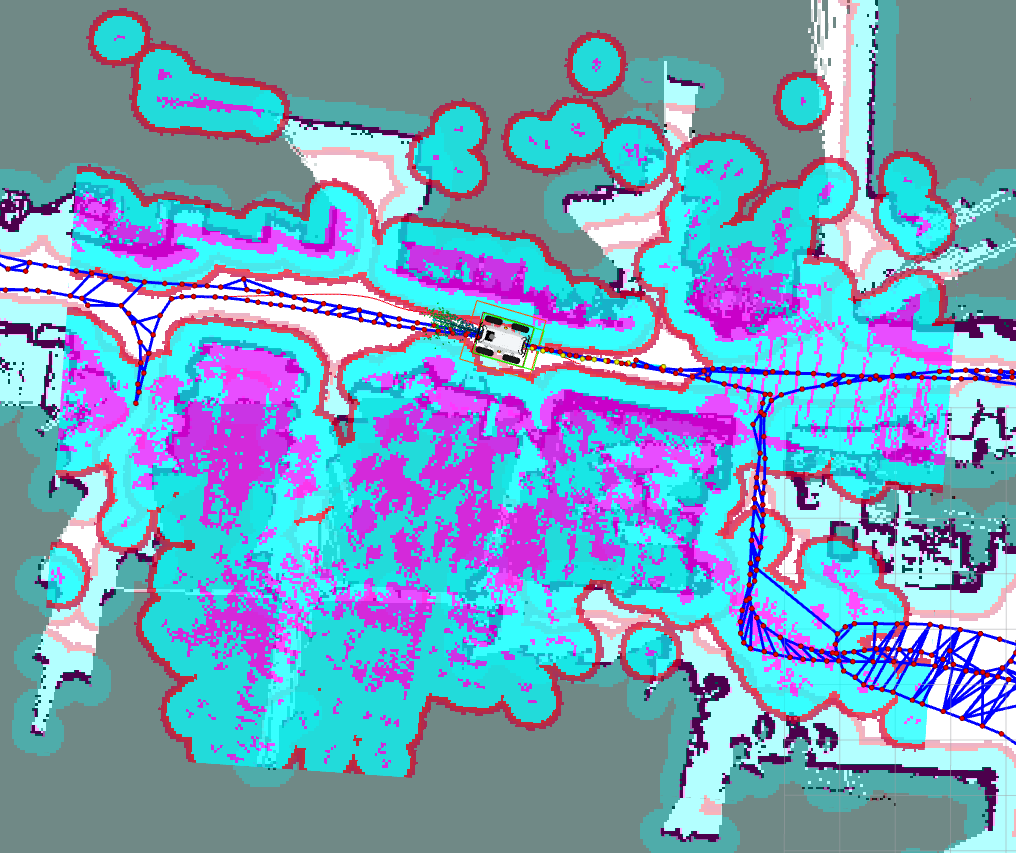
\includegraphics[width=1.0\textwidth]{c4_22.png}
    \caption{Autonomous Navigation in cluttered and dynamic environment with moving obstacles (AIRlab)}
    \label{fig:nav2_airlab}
\end{figure}

\subsection{Nav2 Parameters Tuning}

Finding the right parameters for the Nav2 stack was a challenging task, as the stack has many parameters that need
to be tuned to achieve optimal performance. The parameters to be set are related to all the plugins that are part
of the Nav2 stack. Many tests in different and complex environments were performed to find the best parameters
suitable for the AgileX Scout robot. The parameters were set based on many days of intense testing in both simulated
and real environments, to ensure that the robot can navigate safely and efficiently in different scenarios.

\textbf{Localization Algorithms}:
I tested and applied both AMCL and SLAM Toolbox algorithms for localization, and I found that the AMCL algorithm
performed worse in terms of scan matching when the robot rotates in place. Therefore, I decided to use the SLAM Toolbox
algorithm for localization, which provided better performance and improved reliability in terms of localization accuracy,
even in maps with dynamic obstacles and changing environments. The pose graph generated by the SLAM Toolbox algorithm
is displayed in the maps, as shown in figure \ref{fig:nav2_hallway} and figure \ref{fig:nav2_airlab}, where the
blue lines represent the pose graph created during map creation, and the cyan lines represent the robot's
the path traversed during navigation, estimated by the algorithm, and connected to one of the nodes in the pose graph.

\textbf{Global Planner}:
I tested and used the SMAC planners \cite{macenski2024smac}, in particular the Hybrid A* global planner.
I found that it performed well in generating optimal paths
for the robot to follow, even in cases where an unknown obstacle appears in the environment. The Hybrid A*
global planner uses an A* search algorithm to generate optimal paths for the robot to follow, which allows the robot
to compute efficient paths and adjust quickly to changes in the environment. The Hybrid A* global planner is based on
the motion generation algorithm, which generates kinematically feasible paths for the robot to follow, and the path selection
algorithm, which selects the best path from the sample paths based on the cost function.
The motion generation algorithms available are the \textit{Dubin} and \textit{Reeds-Shepp} algorithms, which both generate
kinematically feasible motion trajectories. After many tests, I found that the Reeds-Shepp algorithm enabled
to generate paths also in the reverse direction, which is useful for navigating in reverse, especially for
a skid-steering drive robot such as the Scout. However, for some reason still unknown to mankind and Steve Macenski,
the Reeds-Shepp algorithm works only in the real environment, and not in the simulated environment in Ignition Gazebo.

\textbf{Local Planner (Controller)}:
I tested and applied the DWB and MPPI local planners, and I found that the MPPI local planner performed better
in tracking the global plan and avoiding tight obstacles. The MPPI (Model Predictive Path Integral Controller) 
\cite{mppicontroller} local planner uses a \textbf{model predictive control approach}
to generate collision-free paths for the robot to follow, which allows the robot to navigate efficiently in complex
environments with tight spaces and obstacles. The MPPI local planner also provides better performance in terms of
trajectory tracking, compared to the DWB local planner. The DWB local planner uses a dynamic window approach to generate
collision-free paths for the robot to follow, which can be less effective in tight spaces and complex environments.
The sampled trajectories of the local planner are visualized in \ref{fig:nav2_hallway} and \ref{fig:nav2_airlab},
in front of the robot's footprint, showing the robot's sampled trajectories to follow the global path.

\textbf{Recovery Behaviors}:
I tested the default recovery behaviors provided by the Nav2 stack, and I found that the default recovery behaviors
performed well in recovering the robot from unexpected scenarios, such as getting stuck or colliding with obstacles.
So I decided to modify slightly the default recovery behaviors to improve the robot's performance in recovering
from the scenarios where the robot would be stuck near an obstacle and unable to move. The modified recovery behaviors
include a combination of back-up and rotate behaviors, which allow the robot to back up and rotate in place to position
itself in a different configuration, enabling it to generate a new path and continue navigating towards the goal.

\textbf{Local Costmap}:
The local costmap plugin is used to generate a local costmap of the robot's surroundings, highlighting obstacles
and free space. The local costmap plugin uses the robot's LiDAR sensor to perceive the environment and update the costmap
in realtime. The local costmap plugin is used by the local planner to generate collision-free paths for the robot
to follow. The local costmap includes the unknown obstacle in the environment, which is represented as pink areas
in the costmap, as shown in figure \ref{fig:nav2_airlab}. The unknown obstacle is detected by the LiDAR sensor
and updated in the costmap, allowing the robot to avoid collisions with objects not present on the map.
The local costmap can be configured with these plugins:

\begin{itemize}
    \item \textbf{Inflation Layer}: The inflation layer is used to inflate the obstacles in the costmap, creating a buffer
    around the obstacles to ensure that the robot avoids collisions.
    \item \textbf{Obstacle Layer}: The obstacle layer is used to update the costmap with the obstacles detected by
    the 2D LiDAR sensor, highlighting the obstacles in the costmap. I later substituted this layer with the voxel layer,
    thanks to the more effective 3D LiDAR sensor perception.
    \item \textbf{Static Layer}: The static layer is used to update the costmap with the static obstacles in the map
    \item \textbf{Voxel Layer}: The voxel layer is used to update the costmap with the voxelized obstacles in the map,
    using the 3D LiDAR sensor to perceive the environment and update the costmap in realtime.
\end{itemize}

\textbf{Global Costmap}:
The global costmap plugin is used to generate a costmap of the entire map that the robot is navigating in, highlighting
the static obstacles and free space. The global costmap plugin is used by the global planner to generate optimal paths
for the robot to follow. The global costmap is configured to use only the static layer inflated by the inflation layer,
to ensure that the robot avoids collisions with the obstacles already present in the map.
The global costmap is represented in \ref{fig:nav2_hallway} as the blue and red areas, where the blue areas are the 
\textit{lethal} space (i.e. must be avoided) and the red areas are the inflated obstacle areas with high cost.

\textbf{Collision Monitor}:
The collision monitor plugin is used to continuously assess the robot's planned path against the costmap, ensuring
that the robot navigates safely and avoids collisions with obstacles. The collision monitor plugin is used by the
nav2 stack to ensure that the robot avoids the obstacles in the costmap, such that they do not overlap with the robot's
footprint and locally planned path.

\textbf{Mapping Algorithm}:
The algorithm of choice for mapping is the \textit{SLAM Toolbox} algorithm, which is a 2D SLAM algorithm
that uses the robot's LiDAR sensor to create a 2D map of the environment \cite{Macenski2021slamtoolbox}.
The SLAM Toolbox algorithm is used to create
a 2D map of the environment, which is used by the global planner to generate optimal paths for the robot to follow.
The SLAM Toolbox proved to be effective in creating accurate 2D maps of the environment, even in dynamic environments
with moving obstacles. I managed to use it correctly in both simulated and real environments, and it provided
good performance in terms of mapping accuracy and reliability.

\textbf{Velocity Smoother}:
The velocity smoother plugin is used to smooth the robot's velocity commands, ensuring that the robot moves smoothly
and efficiently in the environment. The velocity smoother plugin is used by the local planner to obtain smooth
trajectories from the computed paths, which allows the robot to navigate efficiently and avoid jerky movements.
The velocity smoother is configured also to avoid unnecessary stops and starts, which can wear out the robot's transmission
gears and reduce the robot's battery life.

\textbf{Spatio-Temporal Voxel Costmap Layer} \cite{macenski2020stvl}:
The dynamic obstacle avoidance algorithm is a critical component of the Nav2 stack, as it allows the robot to navigate
safely in dynamic environments with moving obstacles. The dynamic obstacle avoidance algorithm uses the robot's LiDAR sensor
to perceive the environment and detect the moving obstacles in realtime. Dynamic obstacles update the local costmap
following different plugins, such as the voxel layer, which is used to update the costmap with the voxelized obstacles
in the environment. The voxel layer uses the 3D LiDAR sensor to perceive the environment and update the costmap.
However, one of the shortcomings of the voxel layer is that it doesn't remove old voxels that correspond to obstacles
that are no longer present in the environment. This leads to false positives in the collision checking, which prevents
the robot from executing the planned trajectory, especially in highly dynamic environments with fast-moving obstacles.
The spatio-temporal voxel costmap layer is an open-source plugin that addresses this issue by updating the costmap
efficiently and accurately. It replaces the traditional voxel grid approach with a \textbf{sparse voxel grid} implemented
using OpenVDB, a \textbf{high-performance C++ library}. This allows STVL to handle large, dynamic environments with ease,
such as the one shown in figure \ref{fig:stvl}, 
reducing computational overhead. By leveraging temporal information and applying a voxel grid filter to sensor data,
STVL can better handle noisy and dense sensor readings, especially in proximity to objects. 
This results in smoother, more reliable navigation and improved robot performance in continuously evolving scenarios.
STVL's adaptability, efficiency, and ability to integrate with various sensor types made it the ideal substitute
for the voxel layer in the Nav2 stack. Figure \ref{fig:nav2_airlab} shows the effectiveness of the STVL in a dynamic
and cluttered environment, such as the AIRLab, where the robot is navigating despite many unknown obstacles 
and moving objects in a tight space.

\begin{figure}[t]
    \centering
    \includegraphics[width=0.8\textwidth]{c4_06.png}
    \caption{STVL in action in a dynamic and cluttered warehouse environment}
    \label{fig:stvl}
\end{figure}


\subsection{Issues with 3D LiDAR for autonomous navigation}

Throughout the development of the project, I encountered several issues with the NAV2 stack.
Sometimes the software crashed at random times, unpredictably, and without any apparent reason.
Some other times the dynamic obstacle avoidance algorithm did not work as expected, causing the robot to collide
with obstacles that were not perceived by the LiDAR sensor in the surrounding environment.
Overall, the robot's navigation stack was not reliable and robust, which was a significant issue for the project's development,
especially for the autonomous navigation tasks in the laboratory's environment (cluttered and dynamic).
Figure \ref{fig:3dlidar} shows the pointcloud generated from a cluttered environment and the expected view 
from a correctly functioning sensors.

\begin{figure}[t]
    \centering
    \includegraphics[width=1.0\textwidth]{c4_18.png}
    \caption{3D LiDAR sensor in a cluttered environment}
    \label{fig:3dlidar}
\end{figure}

After many trials and tests, my supervisor and I discovered that the LiDAR pointcloud data's low and unreliable frequency
was the main cause of all these problems. The LiDAR sensor works at a nominal frequency of $10$Hz. 
The LiDAR sensor was not providing a stable scan rate of $10$Hz, but it was fluctuating between $3$Hz and $8$Hz, 
and only in a few cases, it was able to provide the nominal $10$Hz scan rate.
Once we discovered the source of the problem and ensured that the LiDAR sensor was working correctly
(meaning that the sensor was not malfunctioning or working at a lower but valid data rate), 
we tried to find the culprit of the low and unreliable frequency of the LiDAR sensor.

After many attempts, I found out the cause of the problem: the culprit was the \textbf{router}
used to connect the robot's computer
to the laboratory's network and the internet and the DDS (\textit{Data Distribution Service}) middleware used 
internally by ROS2 for the communication between the nodes in a local network. Basically, the DDS middleware
was configured to broadcast all ROS2 packets and data streams to the laboratory's network, causing delays in the transmission
and packet loss, as the network was not able to handle the high-frequency and heavy-weight data streams of the LiDAR sensor.
In fact, by just unplugging the router from the robot's computer, the LiDAR sensor was able to provide a stable scan rate
of $10$Hz, without any fluctuations or drops in the frequency, since no broadcast packets were sent to the network.
Since the router was necessary for the remote control and monitoring, it was simply just not an option
to unplug it from the robot's computer.

For the correct operation of the localization and obstacle 
avoidance algorithms, it is fundamental that the LiDAR sensor works at a \textbf{stable frequency}, 
without any fluctuations or drops in the scan rate. This requirement is essential because these algorithms rely on the
coherent and continuous data stream for time interpolation and filtering of the pointcloud data.
This is why the LiDAR sensor's low and unreliable frequency was causing the software to crash and malfunction.

The solution was to configure properly the \textbf{DDS middleware} to ensure that all ROS-related nodes and data streams
were handled inside the robot's computer only, and not going through the router and the laboratory's network.
Having the data streams in the local machine only, ensured that the LiDAR sensor's data was not distributed 
among the network, causing delays in the transmission and packet loss, which were the main causes of the low and unreliable
frequency of the LiDAR sensor. Furthermore, we configured ROS2 to use the \textit{Cyclone DDS} middleware, which is a lightweight
and fast DDS implementation, suitable for real-time and high-frequency data streams. This DDS implementation was able to handle
heavy-weight data packets at high frequencies, ensuring that the LiDAR sensor's data was transmitted and received correctly
in its entirety, without any losses or delays in the transmission.

After this configuration, the LiDAR sensor was able to provide a stable scan rate of $10$Hz,
and the software stack was working correctly, without any crashes or malfunctions.
Furthermore, I was also able to test the LiDAR sensor at a higher frequency of $20$Hz, 
with lower resolution, and it was working fine and stable.
This solution was essential also for the correct operation of the IMU sensor for the SLAM algorithm, which required
a stable and continuous data stream of the LiDAR at the moment of startup of the sensor in the software stack. Before the 
fix of the LiDAR sensor's frequency, the IMU sensor was not able to start correctly, due to the lack of data
from the LiDAR sensor, and the computed odometry data was drifting too much to be useful.
Many other algorithms and software benefitted from this fix. The robot's navigation stack was now reliable and robust,
and the autonomous navigation tasks were working correctly and smoothly.


\section{Ignition Gazebo Simulation Environment}

Ignition Gazebo is a useful open-source simulation environment for robotics and autonomous systems.
It provides a realistic and customizable 3D environment for testing and developing robotic algorithms and applications.
Ignition Gazebo is the new version of the Gazebo simulator, which is widely used in the robotics community for simulating
robots and sensors for perception systems. \textbf{Ignition Gazebo} is the simulation environment of choice for the project,
as it proved to be very useful in testing the mobile robot base in simulated environments before deploying the algorithms
on the real robot. Simulating the robot in a virtual environment allows for testing the algorithms in 
a controlled and repeatable environment, without the risk of damaging the real robot or the laboratory environment.
The simulations were essential for the development of the software stack and the navigation algorithms, 
as they allowed for testing
the robot's behavior in different scenarios and environments. It allowed me to tune the navigation stack's parameters
thoroughly and ensure the robot would avoid obstacles and navigate safely.

% add a screenshot of the simulation environment in Ignition Gazebo
\begin{figure}[t]
    \centering
    \includegraphics[width=1.0\textwidth]{c4_12.png}
    \caption{Ignition Gazebo Simulation Environment}
    \label{fig:ignition}
\end{figure}

% Add the created map of the warehouse
\begin{figure}[t]
    \centering
    \includegraphics[width=1.0\textwidth]{c4_14.png}
    \caption{Mobile robot navigating in the simulated warehouse environment}
    \label{fig:warehousenav2}
\end{figure}

The simulated environment in Ignition Gazebo was a \textbf{warehouse} \ref{fig:ignition} 
with various obstacles such as walls, shelves, and boxes,
which the robot had to navigate around to reach its goal. The warehouse environment was designed to be challenging
for the robot, with narrow passages and tight spaces, to test the robot's ability to navigate in complex environments.
Ignition Gazebo also provides the possibility to add dynamic obstacles, i.e. objects not present in the map
already loaded in the simulation environment. This feature was useful for testing the robot's dynamic obstacle avoidance
algorithm, which allows the robot to navigate safely in environments with unknown obstacles.

I was able to simulate also the sensors mounted on the robot, such as a 2D LiDAR and a 3D LiDAR sensor, which were used
for perception and obstacle avoidance. I also tested the robot's localization algorithms, such as AMCL and SLAM Toolbox,
using the simulated odometry data created by the robot's wheels' motion in the simulated environment. Figure 
\ref{fig:warehousenav2} shows the simulated mobile robot navigating in the warehouse environment
while avoiding the boxes and shelves in its path.


\section{Parking Algorithm for Mobile Robot}

I designed a \textbf{parking algorithm} for the mobile robot to autonomously park near a target spot in the laboratory.
The parking algorithm takes as input the location in the map of the target spot that the robotic arm must reach,
and it outputs the parking pose next to the target pose where the mobile robot must park to give the robotic arm
enough space to reach the target. I had to structure and design the algorithm to ensure that the mobile robot
could park in a position where the robotic arm could interact with the target object, without colliding with 
the obstacles in the environment nor with the target object itself. The mobile robot must park so that it 
faces the opposite direction of the target object because the robotic arm is mounted on the back of the robot.

The parking algorithm considers both the robot's footprint and the robotic arm's workspace to ensure that the
robot can park in a position where the robotic arm can reach the target object. 
The algorithm also considers the costmap generated by the navigation stack to compute the optimal parking
pose that minimizes the cost of the footprint, meaning that the robot will be the furthest possible from
the obstacles in its vicinity. 

The parking algorithm is then used by the NAV2 commander APIs to send the parking pose to the robot's navigation stack,
which generates a collision-free path for the robot to follow to reach the parking pose. The robot then executes
the planned trajectory and parks near the computed parking pose. While the mobile robot navigates
autonomously to the parking pose, it publishes feedback data containing its current position and its distance 
from the parking pose. 

The parking algorithm is non-deterministic, meaning that it can compute different parking poses for the same target
pose, depending on the obstacles in the environment. The algorithm is explained in \ref{alg:parking}.

\begin{algorithm}[H]
    \caption{\textbf{Parking Pose Computation Algorithm}}
    \label{alg:parking}
    \begin{algorithmic}[1]
    \Require Target $t = (x_t, y_t, \theta_t)$
    \Require Costmap $C$, Robot's Footprint $F$

    \State $n \gets 50$ \Comment {number $n$ of parking pose candidates $p_c$}
    \State $r \gets 0.4$ \Comment {parking radius in meters from the target position}
    \State $P_{current} \gets$ current robot's position in the map
    \State $V_c \gets \emptyset$  \Comment{list of valid candidate poses}

    \Function{rank}{$p$}
        \State $w_{cost} = 0.5, w_{dist} = 0.2, w_{orientation} = 0.3$ 
        \State $cost = cost(F(p), C)$ \Comment{cost in the costmap for given pose and footprint}
        \State $dist = ||P_{current} - p|| ^2$ \Comment {Euclidean distance between poses}
        \State $orient = | \theta_t - \theta_p |$ \Comment {difference between target and candidate orientation}
        \State \Return $w_{cost} \cdot cost + w_{dist} \cdot dist + w_{orientation} \cdot orient$
    \EndFunction

    \For {$i = 1$ to $n$}
        \State $\phi \sim $\textit{Uniform}$(-\phi_{max}, \phi_{max})$ \Comment {random angle}
        \State $x_c \gets x_t + r \cdot \cos(\theta_t + \phi)$ \Comment {candidate $x$ coordinate}
        \State $y_c \gets y_t + r \cdot \sin(\theta_t + \phi)$ \Comment {candidate $y$ coordinate}
        \State $\psi \sim $\textit{Uniform}$(-\psi_{max}, \psi_{max})$ \Comment {random orientation}
        \State $\theta_c \gets \theta_t + \psi$ \Comment {candidate orientation}
        \State $p_c \gets (x_c, y_c, \theta_c)$ \Comment {candidate parking pose}
        \State \Comment{ discard the poses having their footprint $F$ with lethal cost in costmap $C$}
        \If {\textit{cost}$(C, F(p_c)) \neq $ \textit{LETHAL}}
            \State add $p_c$ to $V_c$
        \EndIf
    \EndFor
    \State $V_{ranked} \gets \left[\textbf{rank}(p_{c,1}), \ldots, \textbf{rank}(p_{c, n_c})\right] 
        \quad \forall p_c \in V_c $
    \State $V_{c} \gets \textit{sorted}(V_{ranked}, V_c) $ \Comment{sort list of candidates by their rank}

    \Repeat 
        \State pick {$P_{candidate} \in V_c$} \Comment{pick parking pose from the highest ranked candidates}
        \If {$\exists$ traversable path from $P_{current}$ to $P_{candidate}$}
            \State save parking pose $P_{parking} \gets P_{candidate}$
        \EndIf
    \Until {a traversable path is found}
    \If {$\exists P_{parking}$}
        \State \textbf{navigate} towards $P_{parking}$ with computed traversable path
    \EndIf
    \end{algorithmic}
\end{algorithm}

Experimental tests were performed to evaluate the accuracy and reliability of the parking algorithm.
The tests were conducted in both simulated and real environments, with different configurations of obstacles
and target poses. The parking algorithm was able to compute effective parking poses in most cases,
but it struggled with tight spaces and narrow passages, where the robot had limited space to park.
The biggest limitation of this algorithm is that it cannot consider the feasible workspace of the robotic arm
when computing the parking pose, which can lead to the robot parking in a position where the robotic arm
cannot reach the target object. This limitation is due to the impossibility of predicting the cartesian
target pose that the cobot will have to reach, as it depends on the object's position and orientation
in the environment. The parking algorithm is a good starting point for further development and improvement
to address these limitations and ensure that the robot can park in a useful position also for the robotic arm.

\section{Aruco Marker Detection and Pose Estimation}

Aruco markers are synthetic square markers with unique black-and-white patterns that can be easily detected
and identified by computer vision algorithms.

Detecting and estimating the pose of an ArUco marker from an image involves a two-step process.
First, the ArUco marker is detected in the image using the ArUco library available in OpenCV. 
This library provides functions to detect various ArUco dictionaries and families. 
Once detected, the marker's corners are extracted, and its unique ID is identified. 
The second step involves estimating the pose of the ArUco marker, which refers to its position 
(translation) and orientation (rotation) with respect to the camera. The function for pose estimation 
takes the detected marker corners, the marker size, and the camera's intrinsic parameters (focal length,
principal point, and distortion coefficients) as input and returns the pose of the marker in the form of a rotation
vector and a translation vector.

The intrinsic parameters of the camera are crucial for accurate pose estimation. These parameters describe the camera's
internal characteristics, such as the focal length, which determines the field of view, and the principal point,
which is the center of the image. The distortion coefficients model the lens distortion, which can cause straight
lines to appear curved in the image. By incorporating these parameters into the pose estimation process,
we can compensate for the camera's inherent distortions and obtain a more accurate estimate of the ArUco marker's pose
in the real world. I had also to calibrate the camera's intrinsic parameters using a calibration pattern and the
automatic calibration software tool provided by the RealSense SDK.

\subsection{Multi-Aruco Plane Estimation Algorithm}

One of the challenges I faced was estimating the orientation of small Aruco markers from the camera feed.
The pose estimation algorithm works well for markers that appear large in the image, but it struggles with
the ones that appear smaller due to the size and distance from the camera. The estimation of the orientation
was the most challenging part, as the pose estimation algorithm often returns orientation values that
oscillate between different values, making it difficult to determine the correct orientation of the marker.
This is especially true for small markers that appear far away from the camera. To address this issue,
I developed a multi-Aruco plane estimation algorithm that estimates the orientation of a plane over which
multiple Aruco markers are placed. Figure \ref{fig:multi_aruco} shows the algorithm in action.

\begin{figure}[t]
    \centering
    \includegraphics[width=1.0\textwidth]{c4_17.png}
    \caption{Multi-Aruco Plane Estimation algorithm in action. The screenshot shows RViz2 displaying
    on the top left corner the input image, bottom left the image with the detected markers drawn on top of it,
    and in the center the colored pointcloud captured by the depth sensor.}
    \label{fig:multi_aruco}
\end{figure}

The algorithm works by detecting multiple Aruco markers in the image and estimating their poses using the pose
estimation algorithm. The poses of the Aruco markers are then used to estimate the orientation of the plane
on which the markers are placed. The algorithm assumes that the Aruco markers are \textbf{coplanar}, meaning that 
they have different positions but the same orientation. By estimating the orientation of the plane that passes
through the markers, we can determine the correct orientation of the markers from the vector normal
to the plane. The algorithm processes a list of Aruco markers poses and returns the poses with their
estimated orientation, meaning that all processed poses share the same orientation value.

The algorithm that I implemented makes use of the following statistical data analysis techniques:

\begin{itemize}
    \item \textbf{RANSAC (Random Sample Consensus)}: RANSAC is an iterative algorithm used to estimate
    the parameters of a mathematical model from a set of observed data points that contain outliers.
    RANSAC works by randomly selecting a subset of data points and fitting a model to them. The model is then
    evaluated against the remaining data points, and the points that are consistent with the model are considered
    inliers. The process is repeated multiple times to find the best-fitting model with the maximum number of inliers.
    RANSAC is used to discard the outlier data points observed in the Aruco markers' poses.
    \item \textbf{Least Squares Estimation (LSE)}: LSE is a mathematical method used to find the best-fitting curve
    that minimizes the sum of the squared differences between the observed data points and the model's predictions.
    LSE is used by the RANSAC model to fit the plane that passes through the Aruco markers' poses.
    \item \textbf{Principal Component Analysis (PCA)}: PCA is a statistical method that identifies patterns
    in data by transforming it into a new coordinate system, where the data points are uncorrelated.
    PCA is used to find the principal components of the data, which are the directions of maximum variance.
    In the context of this algorithm, PCA is used to find the vector passing through points lying on a line.
    It is used as a technique for outlier removal and noise reduction in the data.
    \item \textbf{Singular Value Decomposition (SVD)}: SVD is a matrix factorization technique that decomposes
    a matrix into three matrices, which represent the singular vectors and singular values of the original matrix.
    SVD is used as an optimization technique to find the best-fitting plane that passes through the given points.
    It works as a technique for reducing the dimensionality of the data, by reducing the impact of noisy
    and irrelevant data points.
\end{itemize}

The perception algorithm works as illustrated in \ref{alg:multi_aruco}:

\begin{algorithm}[H]
    \caption{\textbf{Multi-Aruco Plane Estimation Algorithm}}
    \label{alg:multi_aruco}
    \begin{algorithmic}[1]
    
    \Require points $P = \left[ p_1, \ldots, p_n \right]$ with $p_i = (x_i, y_i, z_i)$ coordinates of all points
    \Require collinear points $T = \left[t_1, \ldots, t_n \right]$ with $t_i = (x_i, y_i, z_i)$ assumed to be collinear
    
    \Function{RANSAC}{P}
        \State $\tau \gets 0.01$ \Comment {distance threshold in meters}
        \Repeat
            \State $S =$ random subset of points from $P$
            \State $c =$ centroid($S$) 
            \State $n = SVD(S - c)$  \Comment{Compute SVD from subset of points centered in $0$}
            \State inliers $ = 0$ \Comment{number of inliers for S}
            \ForAll { $s_i$ in $S$}
            \State $d = n \cdot s_i$ \Comment{distance between normal $n$ and point $s_i$}
                \If { $||d|| ^2 < \tau$} \Comment{if point $s_i$ is close enough to the plane defined by $n$}
                    \State inliers $++$
                \EndIf
            \EndFor
        \Until {inliers number is maximized}
        \State \Return $n$ \Comment{Returns normal vector $n$ to the best fitting plane to $S$}
    \EndFunction
    \State
    \State $n$ = \textbf{RANSAC}$(P)$
    \State $c =$ \textit{centroid}($T$) 
    \State $B = $ \textbf{PCA}$(T)$ \Comment{compute \textbf{PCA} of collinear points without centroid}
    \State $d = B[2]$ \Comment{direction of highest variance is the last eigenvector in $B$}
    \State $V_x \gets d, \quad V_z \gets n$
    \State $V_y \gets V_z \times V_x$ 
    \State $Rot = \left[V_x, V_y, V_z \right]$ \Comment{compose 3d rotation matrix from vectors}
    \State $q = $ \textit{rot2quat}$(Rot)$ \Comment{convert rotation matrix to quaternion $q$}
    \State update points in $P$ with the orientation quaternion $q$
    \end{algorithmic}
\end{algorithm}

\section{Object Detection with YOLOv8}

For the project, it was also necessary to detect objects in the environment, such as colored balls, which the robot
had to grasp and move to a different location. For this task, I used the YOLOv8 object detection algorithm, trained
on a custom dataset that I collected and annotated. Figure \ref{fig:balls} shows the YOLOv8 model in inference
in realtime, predicting the colors of the balls in the field of view of the camera.

%Add a picture of the detected balls
\begin{figure}[t]
    \centering
    \includegraphics[width=1.0\textwidth]{c4_16.png}
    \caption{YOLOv8 detecting colored balls in realtime from the RGB camera feed. The screenshot displays the image
    with the bounding boxes colored with the same color as the predicted class. For each prediction, the 
    class probability is associated.}
    \label{fig:balls}
\end{figure}

\textbf{YOLO (You Only Look Once)} is a cutting-edge, real-time object detection algorithm 
that has revolutionized computer vision \cite{redmon2015yolo}.
Unlike traditional methods that require multiple passes over an image, YOLO analyzes the entire image in a single pass,
making it incredibly fast and efficient. It divides the image into a grid and predicts bounding boxes and class probabilities
for each grid cell simultaneously, achieving impressive accuracy while maintaining speed. 
YOLO has evolved through several versions (YOLOv2, YOLOv3, etc.), each improving upon the previous iteration in terms of speed, 
accuracy, and ability to detect small objects. Its versatility and effectiveness have led to widespread adoption in various
applications, including autonomous driving, robotics, and image analysis tools. This was the object detection neural
network of choice for the project, as it provided the speed and accuracy needed for detecting objects in real-time
from the camera feed. It is also lightweight, making it ideal to run on CPUs without the need for a GPU.
The inference time for a single image on an Intel i7 12th gen CPU was around $0.15$ seconds, which is fast enough
for the time requirements of my applications. However, when running along other ROS2 nodes using other CPU-intensive
algorithms, the inference time increased to $0.4$ seconds, which was still acceptable for the demos and tests.

The \textbf{YOLOv8} neural network model is a state-of-the-art object detection model \cite{reis2023realtimeyolov8}
that combines the best features of previous YOLO versions
to achieve superior performance. I used this model for my object detection task, such as detecting colored balls
from the camera feed. The YOLOV8 architecture is shown in figure \ref{fig:yolov8}. It shows the backbone architecture
of the YOLOv8 model, which consists of a series of convolutional layers that extract features from the input image
and pass them to the detection head, which predicts the bounding boxes and class probabilities for the objects in the image.
The backbone architecture used in the training is the default one (CSPDarknet), which is a state-of-the-art backbone.
The neck is a feature pyramid network (FPN) that combines features from different scales to improve the model's
performance in detecting objects of different sizes.

I trained the YOLOv8 model on a custom dataset of colored balls, which included images of the balls
from different angles, distances, and lighting conditions. I collected the dataset using the RealSense camera mounted
on a tripod, which allowed me to capture images of the balls from different perspectives and distances. The dataset
was annotated manually with the bounding boxes and class labels of the balls, which were used to train the YOLOv8 model.
I used the YOLOv8 model provided by \textbf{Keras}, which is a high-level deep-learning library that provides a user-friendly
API for building and training neural networks. Since the training dataset I collected is of small size,
I used data augmentation techniques to increase the dataset's size and diversity, which helped improve the model's
generalization and robustness. The \textbf{data augmentation techniques} included random rotations, translations, and flips
of the images, which created variations of the original images and helped the model learn to detect the balls
from different perspectives and orientations. I included also other types of image augmentation techniques, such as
brightness and contrast adjustments, and Gaussian noise addition, which further increased the dataset's
size and variability. The image augmentation algorithms were implemented using the \textit{Albumentations} library,
which is a powerful image augmentation library for computer vision tasks, specially designed for 
object detection tasks. It is essential to adjust properly the bounding boxes after each image
is augmented, to ensure that the bounding boxes are still correctly positioned around the objects of interest.

% Add the architecture diagram
\begin{figure}[t]
    \centering
    \includegraphics[width=1.0\textwidth]{c4_10.jpg}
    \caption{Architecture overview in detail of the YOLOv8 architecture}
    \label{fig:yolov8}
\end{figure}

As training hyperparameters, I used a batch size of $16$, which is enough for a small dataset such as the one
that I created, a learning rate scheduler with exponential decay, and the early stopping callback to stop the training
when the validation loss stops decreasing. The model is compiled with the Adam optimizer, which is a popular optimizer
for training deep neural networks, and with the YOLOv8 Backbone, which is a state-of-the-art backbone architecture
that provides the best candidate features for object detection tasks. The metrics used to evaluate the model's performance
are the \textbf{mean Average Precision} (mAP) and the \textbf{Intersection over Union} (IoU),
which are standard metrics for object detection tasks. These metrics are incorporated within the COCO evaluation metrics,
which are the standard evaluation metrics provided by the \textbf{KerasCV} library \cite{wood2022kerascv}.

The model is trained with the combination of 2 loss functions:

\begin{itemize}
    \item \textbf{Box Loss}: The box loss function is used to penalize the model for incorrect predictions of the bounding
    boxes of the objects. The box loss function computes the difference between the predicted bounding boxes and the
    ground-truth bounding boxes, using the \textit{CIoU} (Complete Intersection over Union) loss function, which is a
    state-of-the-art loss function that accounts for the object's aspect ratio and orientation \cite{zheng2021ciou}.
    \item \textbf{Class Loss}: The class loss function is used to penalize the model for incorrect predictions of the
    object classes. The class loss function computes the difference between the predicted class probabilities and the
    ground-truth class labels, using the \textit{Binary Cross-Entropy} loss function, which is the loss function of
    choice for multi-class classification tasks that use multi-hot encoded labels instead of one-hot encoded labels.
    After some tests, I switched to the \textit{Binary Penalty Reduced Focal CrossEntropy} loss function, which is a variant
    of the focal loss function that reduces the penalty for misclassifications, and focuses more on the correct
    classification of the objects \cite{law2019cornernet}. This loss function helped improve the model's accuracy.
\end{itemize}

\section{Pose Estimation with Object Detection and Depth Sensing}

The object's pose estimation task involves estimating the position of an object in 3D space using the depth-sensing
camera and the object detection neural network. The object detection algorithm detects the object 
in the RGB image and provides the bounding box coordinates, class label, and confidence score. 
The depth-sensing camera provides the depth map of the scene, which contains the distance of each pixel from the camera.
By combining the object detection results with the depth map, we can estimate the object's position in 3D space
relative to the camera, which is essential for the robot to interact with the object effectively.

This perception algorithm works by creating a \textbf{segmented pointcloud} of the object from the depth map, using the
bounding box coordinates provided by the object detection algorithm, and the projected depth values
from the depth image. This perception algorithm is implemented to estimate the center position
of detected colored balls. 
The segmented pointcloud contains only the points that belong to the object, which are used
to estimate the object's position in 3D space. The segmentation process involves extracting the points within
the bounding box and filtering out the points that are not part of the object using a color mask corresponding
to the predicted class label. The segmented pointcloud is then used to estimate the object's center position
by fitting an ideal sphere of known radius to the segmented points. This center position is then
used to compute the optimal grasping pose for the robot to interact with the object.

This perception algorithm is used to estimate the optimal grasping pose for the robot's end-effector to grasp
the object. The algorithm was first designed to work only with colored balls (of spherical shape),
but I extended it to work with apples too, which are more complex objects with a more irregular shape.


\section{ROS2 Actions Client-Server Architecture for High-Level Tasks}

I leveraged the ROS2 Actions client-server architecture to implement high-level tasks for the mobile manipulation
robotic system. The Action architecture is a powerful and flexible way to define and execute complex tasks
in a distributed system, such as a robotic system. It allows for asynchronous communication between nodes,
enabling the robot to perform multiple tasks concurrently and efficiently. The Actions architecture is based on
the concept of goals, which represent the desired outcome of a task, and results, which represent the task's outcome.
The client sends a goal to the server, which executes the task and returns the result to the client. The client
can monitor the task's progress with the feedback messages and cancel it if necessary, providing a robust 
and reliable way to manage high-level behaviors. The advantage of using the Actions architecture is that it decouples
the task's definition from its execution, allowing for easy reusability and extensibility of the tasks
across different applications. 

The architecture diagram of the ROS2 Actions client-server is shown in figure \ref{fig:actions_architecture}.
The client sends a goal message to the server, which processes the goal and generates feedback messages
to inform the client about the task's progress. The server then sends a result message to the client
once the task is completed. The client can also send a cancel message to the server to stop the task
prematurely. I used this architecture to implement high-level tasks:

\begin{itemize}
    \item \textbf{ROS2 Action Server}: the servers are nodes that handle the task execution, and they are responsible
    for processing the goals, generating feedback messages, and sending the result messages to the clients.
    The servers are implemented on top of the underlying algorithms and functionalities that perform the tasks,
    provided by a separate node inside the same package.
    \item \textbf{ROS2 Action Client}: the clients are nodes that send the goals to the servers, monitor the task's progress
    with the feedback messages, and receive the result messages once the task is completed. The clients are implemented
    as unique nodes that handle the sequence of actions to be executed, decoupled from the underlying algorithms
    and instructions that perform the tasks.
\end{itemize}

\begin{figure}[t]
    \centering
    \includegraphics[width=0.8\textwidth]{c4_07.png}
    \caption{ROS2 Actions Client-Server Architecture}
    \label{fig:actions_architecture}
\end{figure}

\chapter{Experimental Setups and Demonstrations}

This chapter will describe the experiments conducted to demonstrate the capabilities of the mobile manipulation
robotic system. The experiments consist of three demonstrations named "ArUco Follower", "Button Presser", and "Object Picking".
These demos are meant to showcase the capabilities of the robot in various tasks such as following
a marker, pressing buttons, and picking objects. The first demo is a preview of the robotic arm's
autonomous control software. The second demo showcases the capabilities of the entire system in performing
high-level tasks in industrial environments, such as pressing buttons on an industrial control panel.
The third demo is meant to showcase the mobile manipulation capabilities in an agricultural environment, such as picking
fruits.

The experiments are conducted in a controlled realistic environment to test the robustness
and reliability of the system. The demos have been tested inside the Artificial Intelligence and Robotics Laboratory
at Politecnico di Milano. The laboratory has enough space to allow testing the efficiency of the autonomous 
navigation software while testing also the obstacle avoidance algorithm in a cluttered and changing environment.

The objectives of these demonstrations are to evaluate the robot's performance within the
various software components and how well they integrate with the hardware components. The experiments will also
highlight the challenges faced during the development and testing of the robotic system and how they were overcome.
The demos are meant to be a proof of concept of the robotic system's capabilities in simulated scenarios that are as close as
possible to more realistic environments. They are also meant to show the potential of mobile manipulation 
robots in performing various complex tasks that are currently performed by humans. The objective is not to
replace humans but to assist them in performing tasks that are dangerous, repetitive, or require high precision.

\section{ArUco Follower Demo}

The ArUco Follower demo is a demonstration of the robotic arm's autonomous control software. The demo
consists of the robotic arm following an ArUco marker with the end effector. The demo showcases the
motion planning and execution libraries with MoveIt2 and the integration of the ArUco marker detection 
and pose estimation algorithms with the robotic arm's control software.
The demo tests the autonomous control software of the robotic arm in tracking and following a moving target.
Figure \ref{fig:arucofollower} shows the demo in execution, with \textit{MountV1} as end effector (but without
the cylinder presser). The cardboard shown to the camera displays an ArUco marker, tracked by the robotic arm.

In this demo, the end effector, equipped with the camera, will move in a position and orientation that points
toward the center of the
ArUco marker. The algorithm for \textbf{tracking the marker} computes the end effector's target position such that
the arm can always reach it, and the orientation of the end effector is always pointing towards the marker.
The position of the end effector will be exactly the marker's position if the marker is sufficiently close to the arm,
otherwise, the end effector will be positioned to point the camera toward the marker.
If the marker is not visible, the end effector will remain in the last known position until the marker is
visible again. If the marker moves to a different position in the camera frame and stays visible,
the algorithm will compute the new target pose and the end effector will move to it.
The computation of the end effector's target pose is based on geometrical calculations from the marker's position
in the camera frame. The marker's pose is transformed in the robot arm's base frame, and the target pose is
computed based on the robotic arm's workspace. The target pose is then sent to the motion planning and execution
libraries to compute and execute the trajectory to reach the target pose.

A demonstration incorporating the MoveIt2 Servo node for real-time end-effector control via ArUco marker pose
targeting was implemented and tested. However, due to the ongoing development of MoveIt2 Servo at the time of
writing and its associated stability limitations, the resulting trajectories exhibited undesirable jerkiness 
and did not consistently achieve the target pose within a short timeframe. 
Additionally, the requirement for precise PID tuning of the closed-loop joint trajectory controller presented further
challenges in achieving optimal real-time performance. Given these constraints, the decision was made to utilize 
the standard MoveIt2 planning and execution libraries for the final demonstration,
ensuring greater reliability and smoother operation.

% Add a Figure of the ArUco Follower demo setup during testing
\begin{figure}[t]
    \centering
    \includegraphics[width=0.7\textwidth]{c5_19.jpg}
    \caption{ArUco Follower demo during execution. The cardboard shows an ArUco marker.}
    \label{fig:arucofollower}
\end{figure}

\section{Button Presser Demo}

The "Button Presser" demo is a complex demonstration that showcases the potential of mobile manipulation robots
in performing high-level tasks in industrial environments. The demo consists of the robotic arm pressing buttons
on an industrial control panel, in an autonomous way. The objective is to show the capabilities of the robot in performing
tasks that are currently performed by humans. The demo is meant to be a proof of concept of the robotic system's
integration of multiple software components and the orchestration of the robotic arm and mobile base to
interact with the environment without human intervention.
The demo was developed in the context of a larger project in collaboration with a company. The aim of the project is
to use mobile manipulation robots in industrial plants, for monitoring sensors and various equipment,
and intervening in case of emergency, while avoiding human intervention in dangerous environments. 

The purpose is to demonstrate the feasibility of the mobile manipulation robot in interacting with the control panel
autonomously and effectively. It was also important to demonstrate the system's reliability and robustness 
in performing such a complex task, in terms of accuracy in pressing buttons and the time taken to press all the buttons.

\subsection{Buttons Setup Box and End Effector Setups}

For this demo, the \textit{MountV1} was employed, mounted on the robotic arm's end effector. The \textit{MountV1} is a 
custom-designed 3D-printed mount attached to the cobot's flange, which allows the installation of the stereo camera and 
the cylinder presser. The cylinder presser is a cylinder-shaped tool used for pressing buttons.
In \textit{MountV1} the camera is placed in front of the flange, and this resulted in a reduced field of view of the camera.
Despite this camera position, the camera was able to detect the ArUco markers on the control panel
and the buttons to be pressed. Since the \textit{MountV1} proved to be quite effective in the demo, 
the only change made to this version was to shorten the cylinder presser to prevent
the mobility of the end effector from being reduced due to the length of the tool.

Further in the development of the demo, the end effector configuration was switched to \textit{MountV2}, 
which is the next version of \textit{MountV1}. The biggest improvement of \textit{MountV2} is the camera's position, 
which is placed on the wrist of the cobot, allowing a greater field of view of the camera. 
This proved more effective in finding the ArUco markers on the control panel from a closer distance. 

Using \textit{MountV1}, the end effector was slipping during the execution of the linear trajectories, due to the
roundness of the button caps. This is due to the low friction between the digital button and the round button cap,
having both surfaces made of plastic and a small contact area. The slipping of the end effector caused the
robotic arm to fail to press the buttons effectively. To overcome this problem, the end effector was replaced
with \textit{MountV2}, which has a vacuum suction cap on its tip, instead of having a cylinder presser.
The end effector presents a vacuum suction capo used to press the buttons effectively.
This solution is more effective in pressing the buttons, thanks to the greater friction between the plastic
button cap and the silicon suction cup. The vacuum suction cap presses the buttons reliably, with less slipping,
thanks also to the greater contact area between the cap and the button.

%\TODO{add picture comparison between MountV1 and MountV2 end effectors}

The Realsense camera was used only for ArUco markers detection and pose estimation. So the software
component related to the perception of the control panel didn't make use of the infrared cameras for 
depth estimation. The position of the markers is in fact computed using the RGB image as input and
the equations for 3D camera projection on a 2D matrix for the pose estimation.

The control panel is a custom-designed box with three buttons of different sizes and seven ArUco markers
(having dictionary 4x4) placed around the buttons. Figure \ref{fig:buttonsbox} shows the control panel.
The control panel is small and portable and can be placed in any position and orientation to test the robustness
of the system. The control panel has also three different lights, one for each button,
that indicate whenever a button is pressed. 

The reason for having multiple ArUco markers instead of just one or three for the three buttons,
is to have a more robust and reliable detection of the buttons' positions. Having multiple markers
allows the system to detect the buttons' orientation in a more precise way that is also robust to noise.
The markers are placed around the buttons in a way that the plane estimation algorithm can compute
the plane of the markers effectively, relying on a greater number of points to estimate the plane.

\begin{figure}[t]
    \centering
    \includegraphics[width=0.7\textwidth]{c5_05.jpg}
    \caption{Control panel with 3 buttons and ArUco markers.}
    \label{fig:buttonsbox}
\end{figure}

\subsection{End Effector Positioning and Linear Trajectories}

The implementation of the algorithms for pressing buttons and planning the trajectories is handled inside
ROS2 nodes. One ROS2 node subscribes to the ArUco markers detection topic containing the estimated markers' poses 
and their IDs. Given the markers' poses, and the relative positioning of the markers with respect to the buttons,
the node computes the position of the buttons in the robot's base frame. The node also computes the orientation
of the end effector, such that the vector from the arm's flange and the end effector tip
faces the plane of the markers orthogonally, and this is needed to compute the orientation required to press the buttons.

The \textbf{algorithm} for computing the sequence of target poses that the end effector must reach uses the 
\textbf{estimated position and orientation of the buttons}. For each button, the algorithm computes the pose 
immediately above the button, meaning that the end effector faces the button orthogonally from a fixed distance.
Then the algorithm generates the linear path that the end effector must follow to reach the pose where 
the button is pressed. The linear path is then reversed to get the path required to lift the end effector 
from the button in order to release it and return to the starting point above the button. This sequence
of target poses computation is repeated for each button on the control panel. The ROS2 node uses these target 
poses and linear paths to plan and generate the trajectories for the arm to reach the target poses and 
follow the linear paths. Once the trajectory plans are generated, they are executed.

The linear motion trajectory generation is the most challenging part of the trajectory planner,
because the algorithm that computes the trajectories must take into account several constraints,
such as the static collisions with external bodies and the robotic arm's self-collision mapping.
There are two main methods to generate a linear trajectory for the end effector in cartesian space:

\begin{itemize}
    \item \textbf{Cartesian Linear Motion Planning generation via a sequence of waypoints}:
    this method generates a sequence of pose waypoints (sequence of positions and orientation) that the
    end effector must follow to reach the target pose. The trajectory is generated by interpolating
    the sequence of waypoints in space and time. The trajectory planner generates a trajectory that
    follows the waypoints with maximum deviation defined as the \textit{end effector jump}, which is
    the maximum total deviation in joint space that each joint can have from the average joints' positions.
    This parameter controls how much the joints can move from their average configuration during the 
    execution of the linear trajectory. Setting the end effector jump to zero means that the joints
    will not move from their average configuration, and the end effector will follow the waypoints
    exactly.
    \item \textbf{Constrained Cartesian Motion Planning}: this method creates a motion plan request with the
    addition of position and orientation constraints on the end effector that must be respected while moving
    toward the final pose. The constraints are defined as a position box constraint, meaning that the end 
    effector must stay within a box (rectangular cuboid) in the cartesian space, and an orientation constraint,
    defined as a quaternion representing the orientation and the maximum angle of deviation from the
    orientation axis defined by the quaternion.
\end{itemize}

Both methods were tested and implemented successfully to be used with the Igus Rebel cobot.
The constrained cartesian motion planning method proved to be unreliable due to the high probability
of not being able to generate a valid trajectory. Adding only one constraint to the motion plan made
the trajectory planner able to find a solution most of the time. But adding two constraints, one for 
the position and one for the orientation, resulted in failed trajectory generation almost every time.
This limitation is caused by the physical characteristics of the robotic arm. To successfully generate
a constrained cartesian motion plan, the robotic arm must have 7 DoF, while the Igus Rebel cobot has only 6 DoF.
This makes the constrained method not suitable for this robotic arm.
The reason behind this is that constraining a motion plan 
with two constraints for a 6-DoF robotic arm results in an overdetermined system of equations, and the
trajectory planner is not able to find a feasible solution, because the constraints add more equations 
than the number of DoF of the robotic arm, resulting in a system of equations with no feasible solution.

Due to this limitation, only the cartesian linear motion planning method was used to generate linear trajectories
following a sequence of waypoints. The end effector's jump was set to zero to make the end effector follow
the waypoints exactly, to avoid random jumps in the cobot's configuration. The linear trajectories were
generated successfully and executed correctly most of the time. Sometimes the trajectory planner failed
to find a solution, even when attempting to create a trajectory plan multiple times. This was due to the
complexity of the environment that the planner must take into account. After many attempts with 
different motion planners, such as OMPL, STOMP, and the Pilz industrial motion planner, the one that
proved to be the most reliable and robust for generating linear trajectories was the Pilz industrial motion planner.

The \textbf{reliability of the trajectory planner} in generating linear trajectories for the end effector
was a crucial aspect of the demo and posed a challenge during the development and testing of the demo.
The planner failed to find a feasible solution frequently. In order to increase the probability of finding
a feasible solution, an increase in the tolerances of the planner, such as the maximum deviation
of the end effector from the waypoints, and an increase in the number of attempts to generate a trajectory plan
made the planner more reliable.

\subsection{Mobile Button Presser Demo}

The "mobile button presser" demo is a complex demonstration to showcase the mobile manipulation robot's
capabilities in pressing buttons on an industrial control panel autonomously. The demo consists of the mobile
manipulation robot navigating to the control panel's location, detecting the control panel, and pressing the buttons
in a predefined sequence.

The \textbf{complete demo}, illustrated in the flowchart in Figure \ref{mbp_flowchart}, consists of the following steps:
\begin{enumerate}
    \item The mobile manipulation robot starts from a random location and does not know 
    where the control panel is located.
    \item The robotic arm performs an inspection routine using the camera mounted on the end effector
    to search for a specific ArUco marker, which signals where the control panel is located.
    \item Once the specified marker is detected, and its distance is computed, the algorithm computes the
    position of the control panel in the map frame of reference.
    \item The robotic arm parks itself to not obscure the field of view of the LiDAR, which is essential for 
    localization and autonomous navigation.
    \item The mobile base navigates to the control panel's location autonomously, while avoiding obstacles in the
    environment.
    \item The mobile robot parks in front of the control panel at a fixed distance, facing the opposite side of the control panel,
    so that the robotic arm can move freely without colliding with the mobile base and reach the buttons.
    Figure \ref{fig:buttonpresser1} shows this stage of execution of the demo.
    \item The robotic arm uses the onboard camera mounted on the end effector to inspect the close environment
    to search for the ArUco markers on the control panel, indicating the locations of the buttons to be pressed.
    \item Once the camera detects the ArUco markers, the algorithm computes the position and orientation
    of the buttons placed on the panel in the robot's base frame.
    \item For each button, it finds the end effector target poses in the cartesian space required to press the buttons.
    It also creates the linear paths for the end effector necessary to press and release the buttons.
    \item The robotic arm executes the computed trajectories, and the end effector presses the buttons in the predefined sequence.
    Figure \ref{fig:buttonpresser2} shows the end effector pressing one of the buttons, at this stage of execution of the demo.
    \item The control panel lights up the corresponding light for each pressed button.
\end{enumerate}

\begin{figure}[t]
    \centering
    \includegraphics[width=1.0\textwidth]{demo1.png}
    \caption{Flowchart of the Mobile Button Presser demo execution}
    \label{mbp_flowchart}
\end{figure}

\subsection{Mobile Button Presser Demo Implementation and Architecture}
\label{sec:demo1}

This demonstration is handled by one ROS2 node (action client) that orchestrates the actions of the mobile base
and the robotic arm. The client node sends the goal to three different action servers:

\begin{itemize}
    \item \textbf{Parking Action Server}: this server is responsible for computing the parking algorithm, given the
    position of the control panel in the map frame. After the parking pose is computed, the server sends a navigation
    goal to the nav2 stack to navigate autonomously to the parking pose. The action returns the result containing
    information about how close the robot is to the parking pose when the autonomous navigation is completed.
    \item \textbf{Button Finder Action Server}: this server is responsible for searching for a specific ArUco marker
    in the room. The server executes a "searching movement", which is a sequence of predefined poses that the robotic arm
    must follow to search for the marker. The server also executes all trajectories until the marker is detected.
    The server returns once the marker is detected, and the distance from the cobot to the marker is computed.
    \item \textbf{Button Presser Action Server}: this server is responsible for pressing the buttons on the control panel.
    It first computes the "searching movement" to search for the ArUco markers on the control panel.
    Once the markers are detected and the control panel is located, the server computes the target poses and linear paths
    for pressing the buttons. The server then executes the trajectories to press the buttons in the predefined sequence.
    The server keeps track of how many trajectories have been planned and successfully executed, with respect to
    the total number of trajectories to be executed. The server returns the success rate of the executed trajectories.
    The server terminates its execution once all the buttons have been pressed.
\end{itemize}

% Add pictures of the demo execution
\begin{figure}[t]
    \centering
    \includegraphics[width=1.0\textwidth]{c5_10.jpg}
    \caption{Mobile Button Presser Demo in execution}
    \label{fig:buttonpresser1}
\end{figure}

\begin{figure}[t]
    \centering
    \includegraphics[width=1.0\textwidth]{c5_12.jpg}
    \caption{Cobot pressing buttons on the control panel using the \textit{MountV1} end effector}
    \label{fig:buttonpresser2}
\end{figure}

The architecture of the whole system is composed of multiple software components that interact with each other
using ROS2 Actions and Topics. The architecture, shown in Figure \ref{fig:arch1}, is designed to be modular
and scalable, to allow the integration of new components and functionalities in the future.
The architecture is composed of the following macro components:

\begin{itemize}
    \item \textbf{Multi-ArUco Plane Detection and Marker Pose Estimation}: this component is responsible for detecting
    the ArUco markers in the camera's field of view and estimating the markers' poses. The component relies on 
    the Multi-ArUco Plane Detection algorithm to detect the markers and correct their estimated poses using the
    plane estimation algorithm. This algorithm is explained in section \ref{sec:multiaruco}.
    The component publishes the markers' corrected poses on a ROS2 topic.
    \item \textbf{MoveIt2 Servers}: this component includes the MoveIt2 Planning and Execution functionalities
    and the two action servers for finding the parking pose and pressing the buttons. The MoveIt2 servers
    are responsible also for computing and executing the linear trajectories generated by the trajectory planner,
    required to press the buttons. The demo execution pipeline is handled within threads executed 
    on-demand by the MoveIt2 servers, given the goal sent by the client node.
    \item \textbf{Nav2 Servers}: this component is responsible for the autonomous navigation of the mobile base
    using Nav2. It includes also the action server for computing the parking algorithm and the action client
    exploiting Nav2 Commander APIs to send navigation goals to the mobile base. The structure of the parking algorithm
    is explained in section \ref{sec:parking}, while the autonomous navigation integration with ROS2 is explained
    in section \ref{sec:nav2}.
    \item \textbf{Client Node}: this component is responsible for orchestrating the actions of the mobile base
    and the robotic arm. The client node is a ROS2 node that integrates the action clients for the parking, button finder,
    and button presser action servers. The orchestration of the actions is handled by different threads that
    are executed on-demand by the client node, given the goal sent by the user. Multiple threads are present
    since each one is responsible for handling different tests and demo versions.
\end{itemize}

% Add a Picture of the diagram
\begin{figure}[t]
    \centering
    \includegraphics[width=1.0\textwidth]{Mobile Button Presser Demo_updated.png}
    \caption{Architecture diagram of the Mobile Button Presser demo}
    \label{fig:arch1}
\end{figure}


\section{Object Picking Demo}

The "Object Picking" demo is a more complex demonstration that showcases the mobile manipulation robot's capabilities
in picking objects from the environment autonomously. The demo consists of the robotic arm picking colored balls
or apples from an artificial plant, autonomously. The objective is to demonstrate the robotic system's integration of
multiple software components and the orchestration of the robotic arm and mobile base to interact and grasp objects of
different shapes and sizes, using a soft robotic hand gripper.
The soft gripper enables the robotic arm to grasp fragile objects without damaging them, and it is also able to
grasp objects of different shapes and sizes, thanks to the flexibility and adaptability of the silicone fingers.
For this demo, the \textit{MountV2} is used, since it is the only one that supports the soft gripper.

The colored balls used in the demo are small plastic balls of different colors. The balls are used as a
test ground for the grasping capabilities of the soft gripper since they are small enough to be easy to grasp
and the plastic material enables high friction between the fingers and the ball. Instead, the artificial apples
are a little more challenging to grasp, because of their irregular shape.
The artificial apples are used to simulate a realistic and more complex scenario, where the objects to be picked are
closer to objects appearing in real-world environments, such as fruits on trees.

The \textbf{objective of the demo} is to apply the mobile manipulation robot in an agricultural environment, which is
often more challenging and irregular than in industrial environments. The demo is meant to be a proof of concept
of the autonomous control of a robot to pick and place objects in a realistic environment, such as a plantation.

For this demo, three different versions were developed, each with different levels of complexity and challenges.
The first version is used as a test for the algorithm for object pose estimation and the grasping capabilities
of the soft gripper. The second version is a picking task where the manipulator picks up objects and drops them
into a basket positioned on the mobile base, using the neural network for object detection and perception algorithms.
The third version is used to test the robot's navigation and obstacle avoidance capabilities
in conjunction with the object detection neural network and the perception algorithms. In this version,
the task is pick and place, where the placement of the objects is in a predefined location, physically separated
from the picking location.


\subsection{Plants, Colored Balls, and Apples Setup}

The first setup for testing and demonstrating the demo uses a small artificial plant with colored balls attached to it,
as shown in Figure \ref{fig:sim_plant}.
The second more realistic setup uses a large flat surface with artificial apples placed on it, simulating a more realistic
espalier apple tree, as shown in Figure \ref{fig:sim_espalier}.
This sort of tree is used in agriculture to grow apples flatly and vertically, to save space,
and to make the apples more accessible for picking. Figure \ref{fig:real_espalier} shows an espalier apple tree,
grown in a yard.
The apples are placed on the tree at different heights and distances
from each other, to simulate a more realistic scenario where the apples are not all at the same height and distance
from the robot. The apples are also placed in a way that the robot must move around the tree to reach all the apples,
and this is meant to test the robot's navigation and obstacle avoidance capabilities.

% Add a picture of the real plant and the simulated apple tree
\begin{figure}[t]
    \centering
    \begin{subfigure}{0.45\textwidth}
        \includegraphics[width=1\textwidth]{c5_01.jpg}
        \caption{Simulated espalier apple tree}
        \label{fig:sim_espalier}
    \end{subfigure}
    \hfill % Optional: Adds space between images
    \begin{subfigure}{0.5\textwidth}
        \includegraphics[width=1\textwidth]{c5_06.jpg}
        \caption{Real espalier apple tree}
        \label{fig:real_espalier}
    \end{subfigure}
    \caption{Espalier apple trees}
    \label{fig:plants}
\end{figure}

% Add a picture of colored balls on an artificial plant
\begin{figure}[t]
    \centering
    \includegraphics[width=0.5\textwidth]{c5_03.jpg}
    \caption{Magnetic attachment of an apple to the nylon string}
    \label{fig:magnetic}
\end{figure}

The colored balls and apples are attached to the plant with a nylon string. At the extremity of the string, 
a small magnet is secured using two different methods:

\begin{itemize}
    \item \textbf{Version 1 (Hot Glue)}: the magnet is attached to the string with hot glue. 
    For the apples, the magnet is attracted to another magnet placed on a screw that is screwed into the plastic apple. 
    In the case of the colored balls, the magnet is attracted to another magnet glued onto the ball. 
    To enhance robustness, the balls have two magnets: one inside and one glued onto the external surface. 
    Figure \ref{fig:magnetic} shows the magnetic attachment of an apple to the nylon string.
    \item \textbf{Version 2 (3D Printed Magnetic Hook)}: the second iteration replaces the hot glue with a 3D printed hook. 
    This version is designed exclusively for the apples since they can accommodate the screw where the magnet is attached.
    The magnet is securely placed within the hook, without the need for hot glue, and the nylon string is wrapped around it,
    as shown in Figure \ref{fig:hook3dprint}. 
    This eliminates the need for hot glue, which can be unreliable when bonding to magnets, resulting in a more robust attachment.
    The 3D-printed hook is small and lightweight, maintaining the overall design's unobtrusive nature, and 
    ensuring very fast printing times and quick installation. The 3D design is shown in Figure \ref{fig:hookdesign}.
    It is printed in white PLA (Polylactic Acid), making it strong and durable, with a smooth surface finish.
\end{itemize}

Both versions are effective in attaching the objects to the plant and making them detachable without excessive force,
allowing the robotic arm to easily detach them without straining the motors. 
The magnets are small and lightweight, minimally impacting the object's weight and shape. 
The nylon string is thin and transparent, remaining invisible to the camera and preserving the object's appearance.
The key advantage of the 3D printed hook (Version 2) is its enhanced reliability and ease of assembly compared to 
the hot glue method (Version 1).

% Add a picture of the magnetic attachment to apples and balls
\begin{figure}[t]
    \centering
    \includegraphics[width=0.6\textwidth]{c5_04.jpg}
    \caption{Simulated plant with colored balls}
    \label{fig:sim_plant}
\end{figure}

%add screenshot of apple hook 3d print and real apple with hook
\begin{figure}[ht]
    \centering
    \begin{subfigure}{0.55\textwidth}
        \includegraphics[width=1\textwidth]{c5_20.jpg}
        \caption{Magnetic 3D-printed hook on an apple}
        \label{fig:hook3dprint}
    \end{subfigure}
    \hfill % Optional: Adds space between images
    \begin{subfigure}{0.4\textwidth}
        \includegraphics[width=1\textwidth]{c5_22.png}
        \caption{Magnetic hook 3D design}
        \label{fig:hookdesign}
    \end{subfigure}
    \caption{Magnetic hook for attaching apples}
    \label{fig:hook}
\end{figure}

\subsection{DemoV1 with Manual User Input}

This first version of the demo (\textit{DemoV1}) is a test for the grasping capabilities of the soft gripper and
the autonomous control of the robotic arm, without any advanced perception algorithm implemented. 
This demo is also meant to be used when the robotic arm is fixed in a specific location. The demo consists of
the robotic arm picking colored balls from the artificial plant, with manual user input for selecting the target
object to be picked. The user selects the target object by clicking on the object in the camera's field of view,
and the robotic arm moves to the target object's position and grasps it. The user can select only one object at 
a time.

When starting the demo, an image window appears on the screen, showing the camera's RGB image feed.
The user can \textbf{click on the image} and the coordinates of the mouse click are recorded, and broadcast on a ROS2
topic. The object that the user clicks on is assumed that it can be approximated as a sphere.
The algorithm for object position estimation computes the object's position in the camera frame
using the pixel coordinates, the camera's intrinsic parameters, and the depth image from the infrared camera.
The result is a $(x, y, z)$ position vector of the visible point clicked by the user in the camera frame. 
This is the point of the pointcloud on the surface of the object, which roughly corresponds to the 
object's visible surface center. By projecting a ray from the camera's optical sensor to the computed point,
the algorithm computes the object's approximate center in the camera frame. The center is then transformed
into the robot's base frame, and used as input to the grasping pose estimation algorithm to compute the target pose
for the end effector required to position the robot where the object can be grasped.

Once the grasping pose is computed, the robot moves to the target pose and the end effector grasps the object.
The robot then moves to a standard pre-defined position and drops the object, assuming that a basket
is placed exactly underneath the robot's end effector in the dropping position. The robot then returns to the
starting position and waits for the user to select the next object to be picked. Figure \ref{fig:bp1}
shows this demo during its execution, using colored balls as objects to be grasped. The demo worked well
both with the balls attached to the simulated tree and with the ball in the hands of human volunteers, as
in Figure \ref{fig:bp1}.

\begin{figure}[t]
    \centering
    \includegraphics[width=1.0\textwidth]{c5_13.png}
    \caption{Cobot grasping a colored ball from the hand of a volunteer}
    \label{fig:bp1}
\end{figure}

One of the issues faced during the development of the \textit{DemoV1} for ball picking was the \textbf{reflectivity} of the balls
in the \textbf{infrared spectrum} in the presence of strong sunlight. The balls were reflecting the sunlight and the infrared
camera was not able to compute the depth in the spots of the balls' surface with the highest reflectivity. This resulted
in the balls' surface appearing as holes in the depth image. So if the user clicks exactly in the spot where
the ball is very reflective, the depth value computed would be either wrong or infinite and would result in the
algorithm crashing or computing an infeasible grasping pose. This effect was more pronounced with yellow balls.
The immediate solution is to click in the least reflective spots, but this is a temporary workaround and 
not a definitive solution to the problem. \textit{DemoV2} offers a more robust solution to this problem.

\subsection{DemoV2 with Object Detection Neural Network}

In demo version 2 (\textit{DemoV2}), the demo does not require any user input for selecting the object to be picked.
Instead, it relies on a neural network for detecting the objects in the camera's field of view. 
The neural network used for the object detection task is described in section \ref{sec:yolov8}.
The YOLOv8 neural network
is trained to detect the colored balls and the apples, and it outputs the object's bounding box and class label
with the confidence score. The predicted bounding box is used as the starting point to obtain a pointcloud
containing the points on the entire object's surface. The pointcloud is then used to compute the object's center
in the camera frame, and the grasping pose is computed as in the previous version of the demo.
The algorithm \ref{alg:sphere} assumes that the object can be approximated as an ideal sphere of known radius.
This algorithm is very robust for the colored balls, since they are spheres, and less robust and reliable
for the apples, because of their irregular shape. The algorithm is able to compute the object's center
even from a small portion of the object's surface, and this is a key feature of the algorithm because
it does not require the entire object to be visible in the camera's field of view.

DemoV2 solved the infrared reflectivity problem because it relies on the entire pointcloud of the object's surface, and not just
on a single point. This means that even if there is a hole in the pointcloud, the algorithm \ref{alg:sphere} is still able
to compute the object's center correctly (even though likely less precisely).
In the cases where the pointcloud presents points with wrong depth values, the algorithm
is still able to find the correct solution, as RANSAC is robust to outliers and noise in the data.

DemoV2 is programmed to take into account the \textbf{slow performance of the neural network} during inference
on the CPU. The neural network runs on the CPU and it is not able to process the images fast enough to provide
real-time object detection. The neural network takes around 0.5 seconds to process a single image
on the Intel NUC onboard computer, when other algorithms and ROS2 nodes are running in parallel,
especially during the execution of the complete demos. 
Since the task is not time-critical, the neural network can run in the background and provide the predictions
as soon as they are available. The code is implemented with multiple parallel threads that can handle 
and synchronize the data flow between the neural network and the other algorithms.
The code uses the predictions from the neural network coupled with the depth and RGB
images taken at the moment of inference.


\subsection{Mobile Fruit Picking Demos}

\begin{figure}[hpt]
    \centering
    \begin{subfigure}{\textwidth}
        \includegraphics[width=1.0\textwidth]{c5_14.jpg} % Replace with your image file
        \caption{The cobot opens the gripper in the proximity of the apple (at the computed grasping pose) to grasp it}
        \label{fig:mfp1}
    \end{subfigure}
    
    \vspace{1em} % Add some vertical space between images (adjust as needed)

    \begin{subfigure}{\textwidth}
        \includegraphics[width=1.0\textwidth]{c5_17.jpg} % Replace with your image file
        \caption{The cobot grasps the apple from the plant}
        \label{fig:mfp2}
    \end{subfigure}

    \caption{Mobile Fruit Picking demo during execution}
    \label{fig:mfp_}
\end{figure}

The \textbf{complete demo} is based on DemoV2 and extended to include the mobile base's navigation and obstacle avoidance
capabilities. The demo consists of the mobile manipulation robot navigating to the apple tree's location, detecting the apples
using the neural network, and picking the apples in a predefined sequence.
Figure \ref{fig:mfp_} shows different stages of the execution of this demo, where the robot is picking an apple from the tree.
The robot then drops the apples into a basket. There are two versions of the complete demo:

\begin{enumerate}
    \item \textbf{DemoV2 with pick and place on robot}: the robot picks the apples from the tree and drops them on
    a basket that is positioned on the mobile robot base.
    Figure \ref{fig:mobilebasket} shows the basket positioned on the mobile robot base, with the apples collected
    from the tree using the described sequence of actions. The robot does not need to navigate to a separate location
    to drop the apples, but it is sufficient for the robotic arm to move to a predefined position so that
    the end effector is immediately above the basket. This version is simpler and less challenging than the first one,
    but it was implemented to have a demo that is faster to execute and more realistic of a real-world scenario
    where the robot would operate in an agricultural field.
    \item \textbf{DemoV2 with pick and place}: the robot picks the apples from the tree and navigates to a predefined
    location to drop the apples in a basket. The basket is located in a position separate from the tree, and the robot
    must navigate to the basket's location to drop the apples. The robot must avoid obstacles in the environment
    while navigating to the basket's location. This version is more complex and challenging because the robot must
    navigate to two different locations. Once the mobile robot parks next to the basket's location, the robotic
    arm searches with the camera for an ArUco marker, which signals the position of the basket. 
    The basket with the ArUco signal marker is shown in Figure \ref{fig:basket}. Then
    an algorithm finds a feasible pose for the end effector such that it gets placed immediately above the basket,
    where it can release the grip on the grasped object and drop it, as shown in Figure \ref{fig:mfp3}.
    The sequence of actions executed for this demo is shown in the flowchart in Figure \ref{fig:mfp_flowchart}.
\end{enumerate}

\begin{figure}[t]
    \centering
    \includegraphics[width=0.5\textwidth]{c5_21.jpg}
    \caption{Basket positioned on the mobile robot base}
    \label{fig:mobilebasket}
\end{figure}

\begin{figure}[hpt]
    \centering
    \includegraphics[width=0.5\textwidth]{c5_02.jpg}
    \caption{Basket at the dropping location}
    \label{fig:basket}
\end{figure}

\begin{figure}[hpt]
    \centering
    \includegraphics[width=1.0\textwidth]{c5_18.jpg}
    \caption{Cobot dropping the apple in the basket, at the dropping location, during the mobile fruit picking demo}
    \label{fig:mfp3}
\end{figure}

\begin{figure}[hpt]
    \centering
    \includegraphics[width=1.0\textwidth]{demo2.png}
    \caption{Flowchart for the Mobile Fruit Picking Demov2 with pick and place}
    \label{fig:mfp_flowchart}
\end{figure}

The \textbf{object picking routine}, explained in algorithm \ref{alg:picking} is the routine that the robot follows
to pick up objects from a plant. This algorithm is suitable for both apples and colored balls since they are
both approximated as spheres. This routine defines the sequence of actions to be executed by the robot
to search for an object to pick, grasp, and drop in a basket, which can be located either on the robot itself
or in a separate location far from the tree.
The picking routine differs based on the version of the demo. When the robot must place the object
in the basket positioned on the mobile robot itself, or just next to the robot itself, the robotic arm moves to
the dropping pose and drops the object, as explained in the algorithm \ref{alg:picking}. Instead, when the robot
must pick and place in separate locations, the robotic arm moves to its parking position and does not release the object
until the mobile base has reached the dropping location and the camera recognizes the basket using the ArUco marker.

\begin{algorithm}[hp]
    \caption{\textbf{Object Picking Routine}}
    \label{alg:picking}
    \begin{algorithmic}[1]
        \Require Neural Network for object detection \textit{NN}
        \Require Depth Image feed $D$
        \State max object distance $z_{max} = 1.5$ in meters
        \State Generate a list of pose waypoints $W$
        \For {each waypoint $w$ in $W$}
            \State plan and execute trajectory from current pose to $w$
            \State check if there are objects detected by \textit{NN}
            \For {each object $o$ detected by \textit{NN}}
                \State compute \textbf{segmented pointcloud} using algorithm \ref{alg:sphere}
                \State compute centroid point $P$ from segmented pointcloud
                \State compute distance $z$ from centroid $P$
                \State get confidence score $c$ of object $o$ from vector $C$
                \State compute \textbf{priority score} $s = c \cdot 1/4 + (z_{max} - z)/z_{max} \cdot 3/4$
            \EndFor
            \State Choose object $o$ having highest score $s$
        \EndFor
        \State Estimate \textbf{object's center} using algorithm \ref{alg:sphere}
        \State Estimate \textbf{grasping pose} $G$ using algorithm \ref{alg:grasping}
        \If {$\exists$ feasible pose $G$}
            \State compute pre-grasping pose $G'$
            \State plan and execute trajectory to $G'$
            \State \textbf{open the gripper}
            \State plan and execute linear trajectory from $G'$ to $G$
            \State \textbf{close the gripper} to grasp the object
            \State plan and execute linear trajectory from $G$ to $G'$
            \State move back to waypoint $w$
            \State move to dropping pose $d$
            \State \textbf{open the gripper} to drop the object
            \State \textbf{turn off the gripper}
        \Else
            \State move to next waypoint
        \EndIf
    \end{algorithmic}
\end{algorithm}

The algorithm \ref{alg:picking} is the main algorithm that the robot follows to pick objects from the tree.
The algorithm is executed for each waypoint in the list of poses that the robot must follow to search
for objects to pick. If there are multiple objects detected by the neural network in a unique searching pose,
the algorithm chooses the object with the highest priority score, which is computed based on the object's distance
from the robot and the confidence score of the object's detection. The priority score is used to choose the object
that is closest to the robot and has the highest confidence score. The algorithm then computes the object's center
and the grasping pose, and it executes the trajectory to grasp the object. The robot then moves to the dropping pose
and drops the object into the basket. 

\subsection{Mobile Fruit Picking Demo Implementation and Architecture}
\label{sec:demo2}

This complete demo requires the \textbf{integration of multiple software components},
such as the neural network for object detection,
the perception algorithms for computing the object's center, the grasping pose estimation algorithm, the trajectory
planning algorithms, and the navigation and obstacle avoidance algorithms. The demo is a complex orchestration of
multiple algorithms wrapped in ROS2 action servers. The action servers are responsible for executing the actions
and the algorithms required to pick the objects. The action client node is responsible for orchestrating the actions
of the mobile base and the robotic arm, and for sending the goals to the action servers. The action client node
also handles the sequence of actions in case of any failure of any software component and logs the feedback data
received from the action servers. The ROS2 action servers used in the demo are:

\begin{itemize}
    \item \textbf{Parking Action Server}: this server is the same as the one used for the other complete demo.
    The only difference with the other demo is that the location from which the robot must compute
    the parking position is not given by the result of another action, but is read from a configuration file.
    Both poses where to pick objects and the dropping location are hardcoded in a configuration file for
    simplicity and ease of use.
    \item \textbf{Picking Action Server}: this server is responsible for executing the first part of the
    object-picking routine. It is responsible for searching for objects to pick and checking whether there
    exists a feasible grasping pose for the objects in the camera frame. If it finds a feasible grasping pose
    for an object, it plans and executes the trajectories to grasp the object. The server returns the result
    of the planning and execution of the trajectories. It also provides logging feedback about the objects
    detected and the grasping poses computed.
    \item \textbf{Dropping Action Server}: this server is responsible for executing the second part of the
    object-picking routine. It is responsible for moving the robot to the dropping location and dropping the object
    into the basket. This server is called only if the dropping location is separate from the picking location.
    It searches for an ArUco marker signaling the dropping location and computes a feasible pose for the end effector
    to drop the object. Then it moves to that pose and drops the object.
    The server returns the result of the execution of the trajectories and the dropping action.
    It also provides logging feedback about finding the ArUco signaling the dropping location. 
\end{itemize}

The architecture of the whole system is composed of multiple software components that interact with each other
using ROS2 Actions, Services, and Topics. The architecture, shown in Figure \ref{fig:arch2}, is designed to be modular
and scalable, to allow the integration of new components and functionalities in the future.
The architecture is composed of the following macro components:

\begin{itemize}
    \item \textbf{ROS2-Control Gripper Interface}: this component is responsible for actuating the soft gripper,
    using a ROS2 service as an interface to the gripper's ROS2 hardware interface. The hardware interface
    used has a structure analogous to the one used for the control of the robotic arm, as described in 
    section \ref{sec:ros2control}. The ROS2 service is handled by the MoveIt2 APIs node, which provides
    a convenient interface to couple the trajectory planning and execution with the gripper's control,
    necessary for the manipulation tasks.
    \item \textbf{MoveIt2 Servers}: this component includes the MoveIt2 Planning and Execution functionalities
    and the two action servers for finding the parking pose and pressing the buttons. The MoveIt2 servers
    are responsible also for computing and executing the linear trajectories generated by the trajectory planner,
    required for grasping the detected objects. These servers handle also the perception algorithms for computing
    the object's center and the grasping pose, as described in the section \ref{sec:perception}.
    They use the YOLOv8 neural network predictions to execute the pipeline of actions required to pick the objects. 
    The demo execution pipeline is handled within threads executed
    on-demand by the MoveIt2 servers, given the goal sent by the client node.
    \item \textbf{Nav2 Servers}: this component is responsible for the autonomous navigation of the mobile base
    using Nav2. It includes also the action server for computing the parking algorithm and the action client
    exploiting Nav2 Commander APIs to send navigation goals to the mobile base. The structure of the parking algorithm
    is explained in section \ref{sec:parking}, while the autonomous navigation integration with ROS2 is explained
    in section \ref{sec:nav2}.
    \item \textbf{Client Node}: this component is responsible for orchestrating the actions of the mobile base
    and the robotic arm. The client node is a ROS2 node that integrates the action clients for the parking, button finder,
    and button presser action servers. The orchestration of the actions is handled by different threads that
    are executed on-demand by the client node, given the goal sent by the user. Multiple threads are present
    since each one is responsible for handling different tests and demo versions.
    \item \textbf{Neural Network Node}: this component is responsible for running the YOLOv8 neural network
    inference on the RGB images taken by the camera. The neural network node is a ROS2 node that subscribes
    to the RGB image topic and publishes the predictions on a ROS2 topic, as described in section \ref{sec:yolov8}.
    The neural network node is implemented as a wrapper around the Tensorflow model and uses the 
    Tensorflow Python API to load the model and run the inference.
    \item \textbf{ArUco Pose Estimation node}: this component is responsible for computing the ArUco markers' poses
    in the camera frame.
\end{itemize}

% Add a Picture of the diagram
\begin{figure}[ht]
    \centering
    \includegraphics[width=1.0\textwidth]{Mobile Fruit Picking Demo_updated.png}
    \caption{Architecture diagram of the Mobile Fruit Picking demo}
    \label{fig:arch2}
\end{figure}

\chapter{Conclusions and Future Work}

This thesis has presented the development of a mobile manipulator robot capable of performing complex tasks in 
dynamic and unstructured environments. The primary objective of this work is to develop a system that can
autonomously navigate and manipulate objects with different end effector configurations in unstructured environments.
The goal is not to develop a system that works better and faster than humans but to show that an autonomous robotic
system can perform complex tasks that are usually handled by humans. The system is designed to be the working
ground for future research and more complex projects in the field of mobile manipulation.

The agricultural and industrial environments are the main targets for the developed system. Environments such as these
ones are usually dynamic and unstructured, and the tasks that need to be performed are usually repetitive.
This makes them ideal for automation, even though their complexity poses a challenge to the development of autonomous
systems, because the reliability and robustness of the system are crucial for their success.
The demonstrations presented and illustrated in the project, are 

The entire mobile manipulation system developed throughout the project is a proof of concept for the automation of
tasks that are very easy for humans to perform, and common in agricultural and industrial environments,
where the system finds its main applications and use cases. Automating tasks in the agricultural field can lead to significant
increases in productivity and efficiency, especially in environments where the tasks are repetitive and where
there is room for improvement in terms of resource management. Automating tasks in industrial plants instead
can be useful for increasing the safety of the workers, by removing them from dangerous environments, and for
increasing the efficiency of the production lines by diagnosing problems with the sensors mounted on the robot.

The project has been developed with the idea of being a working ground for future research and more complex projects
in the field of mobile manipulation. The code has been written with modularity in mind so that it can be easily
extended and modified to fit the needs of future projects. Several ROS2 packages have been developed as 
a library of tools and functionalities that can be easily integrated into other projects. 

The legacy of this project is thus the codebase and the extensive documentation that has been written throughout
the development of the project. The codebase is a collection of ROS2 packages that can be used as a starting point
for future projects and as a reference for the development of new functionalities. The documentation is a collection
of notes and explanations that can be used to replicate the demonstrations and to understand the codebase,
and how to extend it to create new functionalities. The ROS2 controller for the robotic arm is also a legacy of
this project, as it is the first controller for the robotic arm that has been developed in ROS2 and that can be
operated via ethernet. The hardware setup used for the soft gripper and the pneumatic system is also a legacy of
this project, as it is a working setup that can be integrated into other projects with ease and minimal effort.

% Future work section

Future developments of the project are mainly focused on the improvement of the system in terms of robustness and
reliability, especially in the perception and manipulation software modules. The perception module can be improved by
using more advanced algorithms for object detection and tracking, for example by training the neural network
on a larger dataset and by using more advanced architectures using a GPU for inference. The manipulation module
can be improved by taking into consideration the mechanics and dynamics of the end effector so that the grasping
and manipulation of objects can be more reliable and robust to objects with irregular shapes and different sizes.

The greatest possibilities for improvement are in the autonomous control of the robot arm and the end effector.
The current implementation of the controller is very basic and based on traditional methods with open-source
libraries for trajectory planning and control. The controller can be improved by using more advanced methods
such as deep reinforcement learning or imitation learning techniques, which can be used to learn the control
policy of the entire mobile manipulation system for more complex tasks. The autonomous control with the
methods used throughout the project is limited to tasks that are can be explicitly programmed, and it is not
suitable for tasks that require a high level of dexterity and precision. Instead, future work can focus on
developing a more advanced controller for more complex tasks that are difficult or impossible to be
programmed explicitly. 


%-------------------------------------------------------------------------
%	BIBLIOGRAPHY
%-------------------------------------------------------------------------
\thispagestyle{empty}
\cleardoublepage

\addtocontents{toc}{\vspace{2em}} % Add a gap in the Contents, for aesthetic
\setlength\bibitemsep{0.5\baselineskip}
\printbibliography


%-------------------------------------------------------------------------
%	APPENDICES
%-------------------------------------------------------------------------

\cleardoublepage

% LIST OF FIGURES
\listoffigures

% LIST OF TABLES
\listoftables

% LIST OF Algorithms
\listofalgorithms

% ACKNOWLEDGEMENTS
\chapter*{Acknowledgements}
Here you might want to acknowledge someone.

\cleardoublepage

\end{document}